
\documentclass[11pt,a4paper,oneside]{book}
\usepackage{a4wide}                     % Iets meer tekst op een bladzijde
\usepackage[dutch]{babel}               % Voor nederlandstalige hyphenatie (woordsplitsing)
\usepackage{amsmath}                    % Uitgebreide wiskundige mogelijkheden
\usepackage{amssymb}                    % Voor speciale symbolen zoals de verzameling Z, R...
\usepackage{makeidx}                    % Om een index te maken
\usepackage{url}                        % Om url's te verwerken
\usepackage{graphicx}                   % Om figuren te kunnen verwerken
\usepackage[small,bf,hang]{caption}     % Om de captions wat te verbeteren
\usepackage{xspace}                     % Magische spaties na een commando
\usepackage[latin1]{inputenc}           % Om niet ascii karakters rechtstreeks te kunnen typen
\usepackage{float}                      % Om nieuwe float environments aan te maken. Ook optie H!
\usepackage{flafter}                    % Opdat floats niet zouden voorsteken
\usepackage{listings}                   % Voor het weergeven van letterlijke text en codelistings
\usepackage[round]{natbib}              % Voor auteur-jaar citaties.
\usepackage[nottoc]{tocbibind}		% Bibliografie en inhoudsopgave in ToC; zie tocbibind.dvi
\usepackage{eurosym}                    % om het euro symbool te krijgen
\usepackage{textcomp}                   % Voor onder andere graden celsius
\usepackage{fancyhdr}                   % Voor fancy headers en footers
\usepackage[Gray,squaren,thinqspace,thinspace]{SIunits} % Om elegant eenheden te zetten
\usepackage[version=3]{mhchem}          % Voor elegante scheikundige formules

% Volgend package is niet echt nodig. Het laat echter toe om gemakkelijk elektronisch
% te navigeren in je pdf-document. Deze package moet altijd als laatste ingeladen worden.
\usepackage[a4paper,plainpages=false]{hyperref}    % Om hyperlinks te hebben in het pdfdocument.


%%%%%%%%%%%%%%%%%%%%%%%%%%%%%%
% Algemene instellingen van het document.
%%%%%%%%%%%%%%%%%%%%%%%%%%%%%%

% De splitsingsuitzonderingen
\hyphenation{back-slash split-sings-uit-zon-de-ring}

%\bibpunct{(}{)}{;}{y}{,}{,}             % Auteur-jaar citaties -- zie natbib.dvi voor meer uitleg; niet echt nodig

% Het bibliografisch opmaak bestand.
% ZORG ERVOOR DAT bibliodutch.bst ZICH IN JE WERKDIRECTORY BEVINDT!!!
\bibliographystyle{bibliodutch}

\setlength{\parindent}{0cm}             % Inspringen van eerste lijn van paragrafen is niet gewenst.

\renewcommand{\baselinestretch}{1.2} 	% De interlinie afstand wat vergroten.

\graphicspath{{figuren/}}               % De plaars waar latex zijn figuren gaat halen.

\makeindex                              % Om een index te genereren.

\setcounter{MaxMatrixCols}{20}          % Max 20 kolommen in een matrix

% De headers die verschijnen bovenaan de bladzijden, herdefinieren:
\pagestyle{fancy}                       % Om aan te geven welke bladzijde stijl we gebruiken.
\fancyhf{}                              % Resetten van al de fancy settings.
\renewcommand{\headrulewidth}{0pt}      % Geen lijn onder de header. Zet dit op 0.4pt voor een mooie lijn.
\fancyhf[HL]{\nouppercase{\textit{\leftmark}}} % Links in de header zetten we de leftmark,
\fancyhead[HR]{\thepage}                % Rechts in de header het paginanummer.
% Activeer de volgende lijn en desactiveer de vorige om paginanummers onderaan gecentreerd te krijgen.
%\fancyhf[FC]{\thepage}                  % Paginanummers onderaan gecentreerd.

% PDF specifieke opties, niet strict noodzakelijk voor een thesis.
% Is hetgeen verschijnt wanneer je in acroread de documentproperties bekijkt.
\hypersetup{
    pdfauthor = {Gaspard Lequeux},
    pdftitle = {Een Introductie tot het Zetsysteem LaTeX},
    pdfsubject = {Cursus LaTeX opgebouwd als typevoorbeeld voor het schrijven van een thesis.},
    pdfkeywords = {LaTeX, zetsysteem, thesis, eindwerk}
}


% Het volgende commando zou ervoor moeten zorgen dat er een witte ruimte wordt gelaten tussen
% elke paragraaf. Het zorgt ervoor dat er echter teveel witte ruimte komt boven en onder de
% verschillende titels, gemaakt met \section, subsection...
%%\setlength{\parskip}{0ex plus 0.3ex minus 0.3ex}

% Vandaar dat we expliciet aangeven wanneer we wensen dat een nieuwe paragraaf begint:
% \par zorgt ervoor dat er een nieuwe paragraaf begint en
% \vspace zorgt voor vertikale ruimte.
\newcommand{\npar}{\par \vspace{2.3ex plus 0.3ex minus 0.3ex}}

%%%%%%%%%%%%%%%%%%%%%%%%%%%%%%
% Nieuwe commando's
%%%%%%%%%%%%%%%%%%%%%%%%%%%%%%

% De differentiaal operator
\newcommand{\diff}{\ensuremath{\mathrm{d}}} 

% Super en subscript
\newcommand{\supsc}[1]{\ensuremath{^{\text{#1}}}}   % Superscript in tekst
\newcommand{\subsc}[1]{\ensuremath{_{\text{#1}}}}   % Subscript in tekst

% Chemische formule font:
\newcommand{\ch}[1]{\ensuremath{\mathrm{#1}}\xspace}	 
% Chemische pijl naar rechts:
\newcommand{\chpijlr}{\ensuremath{\hspace{1em}\longrightarrow\hspace{1em}}}
% Chemische pijl naar links:
\newcommand{\chpijll}{\ensuremath{\hspace{1em}\longleftarrow\hspace{1em}}}
% Chemische pijl naar links en rechts:
\newcommand{\chpijllr}{\ensuremath{\hspace{1em}\longleftrightarrow\hspace{1em}}}

\newcommand{\vt}[1]{\ensuremath{\boldsymbol{#1}}} % vector in juiste lettertype
\newcommand{\mx}[1]{\ensuremath{\mathsf{#1}}}	  % matrix in juiste lettertype

% Het latex logo in een eenvoudiger commando steken
\newcommand{\latex}{\LaTeX\xspace}

% Het BibTeX logo
\newcommand{\bibtex}{\textsc{Bib}\TeX\xspace}

% Niew commando om bestandnamen anders weer te geven
\newcommand{\bestand}[1]{\lstinline[basicstyle=\sl]{#1}\xspace}

% Niew commando om commando tekst weer te geven
\newcommand{\command}[1]{\lstinline[basicstyle=\tt]{#1}\xspace}
\newcommand{\commandx}[1]{\index{#1}\lstinline[basicstyle=\tt]{#1}\xspace}

%\lstset{morecomment={\%}}
% Commando om latex commando`s weer te geven (x: voor indexing)
%\newcommand{\lcommand}[1]{\lstinline[basicstyle={\tt},{language=[LaTeX]TeX}]{#1}\xspace}
\newcommand{\lcommand}[1]{\lstinline[basicstyle={\tt}]{#1}\xspace}
\newcommand{\lcommandx}[1]{\index{#1}\lstinline[basicstyle=\tt]{#1}\xspace}


% Niew commando om vreemde taal weer te geven (hint: dit commando kan gebruikt
%   worden om latijnse namen, die ook cursief moeten staan, weer te geven.
\newcommand{\engels}[1]{\textit{#1}\xspace}
\newcommand{\engelsx}[1]{\index{#1}\textit{#1}\xspace}

% Niew commando om iets te benadrukken en tegelijkertijd in de index te steken.
\newcommand{\begrip}[1]{\index{#1}\textbf{#1}\xspace}

% Nieuw commando om figuren in te voegen. Gebruik:
% \mijnfiguur[H]{width=5cm}{bestandsnaam}{Het bijschrift bij deze figuur}
\newcommand{\mijnfiguur}[4][ht]{            % Het eerste argument is standaar `ht'.
    \begin{figure}[#1]                      % Beginnen van de figure omgeving
        \begin{center}                      % Beginnen van de center omgeving
            \includegraphics[#2]{#3}        % Het eigenlijk invoegen van de figuur (2: opties, 3: bestandsnaam)
            \caption{#4\label{#3}}          % Het bijschrift (argument 4) en het label (argument 3)
        \end{center}
    \end{figure}
    }

% Nieuw commando om figuren in te voegen. Gebruik:
% \mijnfiguur[H]{bestand-tabular}{Het bijschrift bij deze tabel}    
\newcommand{\mijntabel}[3][ht]{             % Het eerste argument is standaar `ht'.
    \begin{table}[#1]                       % Beginnen van de table omgeving
        \begin{center}                      % Beginnen van de center omgeving
            \caption{#3\label{#2}}          % Het bijschrift (argument 3) en het label (argument 2)
            \input{#2}                      % Invoer van de tabel
        \end{center}
    \end{table}
    }

%%%%%%%%%%%%%%%%%%%%%%%%%%%%%%
% Nieuwe wiskunde operatoren
%%%%%%%%%%%%%%%%%%%%%%%%%%%%%%

\DeclareMathOperator{\integ}{Integraal}

%%%%%%%%%%%%%%%%%%%%%%%%%%%%%%
% Nieuwe omgevingen
%%%%%%%%%%%%%%%%%%%%%%%%%%%%%%

% Een soort theorem omgeving
\newtheorem{levensles}{Levensles}[chapter]

% Om minder belangrijke delen iets kleiner te zetten.
\newenvironment{MinderBelangrijk}{\small}{}

% Een nieuwe omgeving om letterlijke latex tekst weer te geven.
\lstnewenvironment{llt} 
    {
    \vspace{1.2ex plus 0.5ex minus 0.5ex}   % Beetje ruimte voor de letterlijke tekst
    \lstset{                                % Enkele opties:
        basicstyle={\small\tt},             % Iets kleiner
        %language=[LaTeX]{TeX},              % Syntax highlighting
        stepnumber=0,                       % De lijnen worden niet genummerd
        breaklines=true,                    % Als een lijn te lang is, wordt hij afgebroken
        basewidth={0.5em},                  % Breedte van een letter
        xleftmargin=1em}                    % Inspringing van de linker marge
    }
    {\vspace{0.9ex plus 0.5ex minus 0.5ex}  % Beetje ruimte na de letterlijke tekst
    }

% Een nieuwe omgeving om algemene letterlijke tekst weer te geven.
\lstnewenvironment{lt} 
    {
    \vspace{1.2ex plus 0.5ex minus 0.5ex}   % Beetje ruimte voor de letterlijke tekst
    \lstset{                                % Enkele opties:
        basicstyle={\small\tt},             % Iets kleiner en typmachine lettertype
        stepnumber=0,                       % De lijnen worden niet genummerd
        breaklines=true,                    % Als een lijn te lang is, wordt hij afgebroken
        basewidth={0.5em},                  % Breedte van een letter
        xleftmargin=1em}                    % Inspringing van de linker marge
    }
    {\vspace{0.9ex plus 0.5ex minus 0.5ex}  % Beetje ruimte na de letterlijke tekst
    }



%%%%%%%%%%%%%%%%%%%%%%%%%%%%%%
% Einde van de preamble.
% Begin van de body:
%%%%%%%%%%%%%%%%%%%%%%%%%%%%%%

\begin{document}

\frontmatter

%  Titelblad

\begin{titlepage}

\fontsize{12pt}{14pt}\selectfont

\begin{center}

% Het logo van de Universiteit Gent

\includegraphics[height=3cm]{figuren/ruglogo}

\vspace{1cm}

\fontsize{14pt}{17pt}\selectfont
% De Faculteit:
\textsc{Faculteit Landbouwkundige\ldots err\ldots\\\textsc{Zeus} Werkgroep Informatica}
\fontsize{12pt}{14pt}\selectfont
\vspace{0.3cm}

\vspace{1.2cm}

%Het academiejaar: aanpassen!
Academiejaar 2005--2006

\vspace{2.8cm}

\fontsize{17.28pt}{21pt}\selectfont

% De titel van de thesis:
{\textsc{Een Introductie tot het\\ Zetsysteem \LaTeX}}

\fontseries{m}
\fontsize{12pt}{14pt}\selectfont

\vspace{3cm}

% De auteur van de thesis:
Gaspard \textsc{Lequeux}	

\vspace{1.6cm}

% De promotor van de thesis:
Promotor: Prof.~dr.~A.~Armagneau\\

\vspace{2cm}

% De functie van de thesis:
Scriptie voorgedragen tot het behalen van de graad van\\
\textsc{Goeroe in de \LaTeX ologie}

\end{center}
\end{titlepage}

\thispagestyle{empty}
                            % Algemene versie
%%  Titelblad

\begin{titlepage}

\fontsize{12pt}{14pt}\selectfont

\begin{center}

% Het logo van de Universiteit Gent

\includegraphics[height=3cm]{figuren/ruglogo}

\vspace{1cm}

\fontsize{14pt}{17pt}\selectfont
% De Faculteit:
\textsc{\textsc{Zeus} Werkgroep Informatica}
\fontsize{12pt}{14pt}\selectfont
\vspace{0.3cm}

\vspace{2.5cm}

%Het academiejaar: aanpassen!
Academiejaar 2005--2006

\vspace{3cm}

\fontsize{17.28pt}{21pt}\selectfont

% De titel van de thesis:
{\textsc{Een Introductie tot \LaTeX}}

\fontseries{m}
\fontsize{12pt}{14pt}\selectfont

\vspace{4.2cm}

% De auteur van de thesis:
Gaspard \textsc{Lequeux}	

\vspace{1.6cm}

% De promotor van de thesis:
%Promotor: Prof.~dr.~A.~Armagneau\\

\vspace{2cm}

% De functie van de thesis:
%Scriptie voorgedragen tot het behalen van de graad van\\
%\textsc{Goeroe in de \LaTeX ologie}

\end{center}
\end{titlepage}

\thispagestyle{empty}
                  % Versie 2de kan informatica bio-ir

\mbox{}\vspace{12cm}

{
\footnotesize
Copyright 2003, 2004, 2005, 2006, 2007, 2008 Gaspard Lequeux. 
Alle rechten voorbehouden.
Dit werk mag worden verveelvoudigd en/of openbaar gemaakt door middel van druk, fotokopie, microfilm, geluidsband, kleitabletten, elektronische of welke andere wijze ook, onder de volgende voorwaarden:

\begin{itemize}
\item Vermelding van de auteur.
\item Niet commercieel. Dit vloeit voort uit het feit dat sommige paragrafen overgenomen werden uit \citet{vanOostrum96}, wiens werk niet mag gebruikt worden voor commerci�le doeleinden.
\item Als je dit werk wijzigt en/of verdeelt, moet dit gebeuren onder dezelfde voorwaarden. %Uitgeverijen mogen dus dit werk verbeteren en in boekvorm uitbrengen, maar mogen het kopi�ren van dat boek niet verbieden. % Deze zin is fout: commercieel gebruik is niet toegelaten!!!
\end{itemize}
\npar
\npar
De auteur is niet aansprakelijk voor eventuele fouten en onvolledigheden in dit werk. 
\npar
\npar
Versie 0.6.0\\
Gecompileerd op: \today
}

%
% Typisch copyright voor een thesis.
% Te plaatsen juist na het titelblad.

\rule[-0.4\baselineskip]{0cm}{10\baselineskip}   
\par \vspace{2.3ex plus 0.3ex minus 0.3ex}
De auteur en promotor geven de toelating deze scriptie voor consultatie beschikbaar te stellen en delen ervan te kopi�ren voor persoonlijk gebruik. Elk ander gebruik valt onder de beperkingen van het auteursrecht, in het bijzonder met betrekking tot de verplichting uitdrukkelijk de bron te vermelden bij het aanhalen van resultaten uit deze scriptie.
\par \vspace{2.3ex plus 0.3ex minus 0.3ex}
The author and promoter give the permission to use this thesis for consultation and to copy parts of it for personal use. Every other use is subject to the copyright laws, more specifically the source must be extensively specified when using from this thesis.
\par \vspace{2.3ex plus 0.3ex minus 0.3ex}
Gent, Juni 2004 % Vul de juiste datum in!!!
\par \vspace{2.3ex plus 0.3ex minus 0.3ex}

De promotor \hfill De begeleider \hfill De auteur
\npar
\vspace{2cm}
\npar
% Pas de volgende lijn aan!!!
Prof. dr. ir. A. Armagneau \hfill Zijnen assistent \hfill Gaspard Lequeux

\thispagestyle{empty} 

                   % Voor een echte thesis.
\newpage
%\mbox{}\vspace{-1cm}
%\thispagestyle{plain}

%\textbf{\Huge{Woord vooraf}}

\chapter*{Woord vooraf}

%\vspace{2cm}

\begin{slshape}

%\small
Deze cursus werd in November 2003 voor het eerst uitgegeven in het kader van een Zeus (Studenten Werkgroep Informatica) initiatief om thesistudenten te helpen hun thesis in een aantrekkelijke vorm te gieten. De tekst is opgevat als een soort minithesis zodat studenten gemakkelijk alles kunnen overnemen. Om die reden zijn de bronbestanden beschikbaar gemaakt op het internet.\footnote{\url{http://zeus.ugent.be/~gaspard/latex}} 
\npar
Hoewel sommige deeltjes van deze cursus expliciet gericht zijn op het maken van een thesis, kan de tekst gebruikt worden als algemene inleiding op \latex. In 2004 zag ook Prof. Ottoy dit in. Vandaar dat deze cursus nu deel uitmaakt van de lessen informatica in de tweede bachelor bio-ir van de Universiteit Gent. Bij die gelegenheid heeft hij de cursus volledig nagekeken op taalfouten, waarvoor dank.
\npar
In 2006 heeft Prof. Dawyndt de cursus ook grondig herlezen en nagekeken, waarvoor dank. Sindsdien wordt deze cursus gebruikt in de lessen Computergebruik gegeven in de eerste bachelor Informatica van de Universiteit Gent.
\npar
Voor het schrijven van deze handleiding \latex, werd gebruik gemaakt van twee werken: \textsf{A guide to \latex} van \citet{kopka99} en \textsf{Handleiding \latex} van Piet van Oostrum (1996). Uit dit laatste werden zelfs hele paragrafen overgenomen. Daarnaast werd natuurlijk rijkelijk geput uit de documentatie die meegeleverd wordt met \latex zelf.
\npar
Minder belangrijke delen worden in een kleiner lettertype weergegeven. Verder zijn er verschillende voetnoten die verwijzen naar \latex documentatie op een Debian GNU/Linux systeem. Niemand gebruikt dat natuurlijk. Maar de bedoeling ervan is dat de lezer weet dat de documentatie bestaat, welke bestandsnaam die heeft en waar ongeveer die te vinden is in de \latex directorystructuur. Het is dan niet zo moeilijk meer om in je favoriete besturingssysteem te zoeken naar de desbetreffende bestandsnaam. 
\npar
In een standaard MikTeX installatie (d\'e \latex distributie voor Windows), zijn de helpfiles van de verschillende \latex packages te vinden in \bestand{C:\\texmf\\doc\\latex}. In \bestand{C:\\texmf\\doc\\guides} zijn enkele algemene handleidingen te vinden over \latex.
\npar
Het woord vooraf dient ook om mensen te bedanken: 

\begin{itemize}

\item De mensen van Zeus, voor de stimulerende Vrije--\engels{Open Source} sfeer en het organiseren van lessen hier rond. 

\item Schamper, het studentenblad van de Universiteit Gent, voor het leveren van de promotor van dit werk.

\item Rudy Gevaert, die in het academiejaar 2001-2002 als eerste een \latex les gaf.

\item Geert Vernaeve, voor het eerste contact met \latex en het C-voorbeeld op bladzijde \pageref{cvoorbeeld}.

\item Mensen die fouten rapporteerden en/of verbeteringen suggereerden: David De Wolf, Annelies Huyck, Yves Nevelsteen, Stijn Gors, Geert Vernaeve, Michiel Meire, Hendrik Maryns, Olivier Verhoogen, Jean-Pierre Ottoy, Hugo Coolens, Lieven Clement, Andy Peene, Reinout Debergh, Frederik De Schrijver, David van der Ha, Brecht Donckels, Dominique Lebbe, Christopher De Dobbelaere, Paul Vogels, Heidi Vanparys, Stijn Depuydt, Veerle Gevaert, Joke Van Hevele, Katrien De Dauw, Francis Santens, Nicolas Vanden Bossche en Peter Dawyndt.

\item De (thesis)studenten van het Boerenkot,
%\footnote{Ook nog wel Faculteit Landbouwkundige en Toegepaste Biologische Wetenschappen genoemd, maar niemand gebruikt die lange naam ;-)}
die in 2003 gevraagd hebben naar deze handleiding.

\end{itemize}

\latex lijkt in het begin moeilijk: alles in tekstmode, geen knopjes, je moet speciale commando's kennen om iets te bereiken~\ldots\ De eerste dagen zul je inderdaad enkele problemen ondervinden. Zoeken, doorbijten en hulp vragen aan meer ervaren gebruikers zullen ervoor zorgen dat je na enkele weken zelfs je wiskundige redeneringen rechtstreeks in \latex uitvoert. 
\npar
Deze handleiding is waarschijnlijk niet fautloos. Het rapporteren van meer dan ��n fout, zorgt voor je naam in de volgende editie van dit woord vooraf. Ook inhoudelijke opmerkingen zijn steeds welkom.

\vspace{4ex}

\hfill Gaspard Lequeux

\hfill Gent 9 Augustus 2006

%\normalsize
\end{slshape}

                      % Algemene versie
%\input{lc-woordvooraf-boerenkot}            % Versie 2de kan informatica bio-ir

% Voor een echte thesis, komt hier de samenvatting...
%\input{samenvatting}                       % ...in het Nederlands en...
%\input{summary}                            % ...in het Engels.

% De lijnen van de inhoudsopgave iets dichter op elkaar, niet echt nodig voor de thesis, maar 
% voor dit werk kregen we anders een laatste bladzijde met 3 items op.
\renewcommand{\baselinestretch}{1.08} 	% De interlinie afstand wat vergroten.
\small\normalsize                       % Nodig om de baselinestretch goed te krijgen.
\tableofcontents
\renewcommand{\baselinestretch}{1.2} 	% De interlinie afstand wat vergroten.
\small\normalsize                       % Nodig om de baselinestretch goed te krijgen.

\mainmatter

% De verschillende hoofdstukken:

\chapter{Inleiding}

\section{Hoe het begon}

\subsection{\TeX}

\TeX\ (uitspraak ``Tech'' als in techneut, kan ook als `TeX' geschreven
worden) is een computer-progamma van Donald E.~\citet{texbook}.  Het
is speciaal ontworpen voor het zetten en drukken van wiskundige teksten
en formules. Een belangrijk kenmerk van \TeX\ is dat je er zelf nieuwe functies in kan programmeren (zogenaamde macro's). Het pakket is dus uitbreidbaar. Vele mensen die uitbreidingen geschreven hebben, maken die publiek beschikbaar. Het is dus aangewezen om eerst te kijken wat er al bestaat, vooraleer zelf iets te implementeren.

\subsection{\LaTeX}

\LaTeX\  (uitspraak ``Lah-tech'',
kan ook als `LaTeX' geschreven worden)
is een zogenaamd macro-pakket dat door Leslie \cite{lamport94} werd
geschreven en gebruik maakt van \TeX.
Het stelt de auteur in staat zijn publicaties op eenvoudige wijze en met
gebruik van een op voorhand opgegeven structuur, met boekdrukkwaliteit te
zetten en af te drukken.
\npar
Om die speciale zes \LaTeX\ letters te krijgen, moet je het commando \lcommand{\\LaTeX\\} gebruiken. \TeX\ verkrijg je met het commando \lcommand{\\TeX\\}.

\section{Het verwerken van tekst}

Het maken van printbare documenten kan op verschillende manieren gebeuren. Enerzijds heb je de wuziwuk\footnote{Wat U Ziet Is Wat U Krijgt} tekstverwerkers, waar het merendeel van de mensen mee vertrouwd is, en anderzijds heb je de zogenaamde \engels{markup} tekstprocessing programma's, zoals \latex.
\npar
De wuziwuk tekstverwerkers zijn initieel gemakkelijk in gebruik. Je typt en er verschijnt juist hetzelfde als hetgeen op papier zal komen.\footnote{Althans, dit is de theorie. In de praktijk durft dit wel eens lelijk tegen te vallen.} Voor korte documenten is dit zeer gemakkelijk. Maar voor lange documenten werkt dit niet meer zo goed: die drie enters die je op het einde van een bladzijde had gezet om de daarop volgende titel op een nieuw blad te krijgen (omdat dat mooi was) blijken na het doorvoeren van een verbetering plots in het midden van een blad te staan. Of de figuren die zo mooi geschikt waren, beginnen rond te zweven, of nog erger: worden vervangen door een rood kruis. Zelfs als dat je bespaard wordt, blijft er nog altijd het probleem van consistentie: bij de ene figuur heeft het bijschrift lettergrootte 10, bij de andere 11.
\npar
Vandaar de andere manier: \latex. De opmaak wordt gescheiden van de inhoud. De auteur geeft de structuur aan en de computer maakt aan de hand van de gestructureerde tekst een prettig leesbaar document. Dit kan een printbaar bestand zijn (met \command{latex}) of een webpagina (met \command{latex2html}). Met ��n commando kan je je thesis publiceren op het www!
\npar
De tekst wordt getypt in een gewone editor. In een editor kun je alleen tekst typen: geen knopjes om vet of cursief te zetten, geen animaties, geen figuren invoegen. Enkel tekst, platte tekst. Dit lijkt archa�sch, omdat de meeste mensen alleen \engels{wordpad} als editor kennen, maar er bestaan veel betere: \commandx{vim} is er ��n van, \commandx{emacs} is een andere. Beiden zijn vrij verkrijgbaar op het net. Onder Windows bestaat er zoiets als \engels{winedit} (te betalen) maar ook \command{vim} kan daar ge�nstalleerd worden. D� \latex-editor onder Windows is echter TeXnicCenter.\footnote{\url{www.texniccenter.org}}
\npar
Platte tekst. Da's niet veel. Hoe krijg je dan titeltjes, paginanummering, opmaak? Wel, er bestaan van die regels om goede teksten te maken. Die kun je vanbuiten leren en dan toepassen in een wuziwuk programma. Maar die regeltjes toepassen kan je ook laten doen door de computer. In \latex zeg je: dit is een hoofdstuk, dit een titel, dit is een belangrijk woord, dit is letterlijke tekst, in de buurt van deze paragraaf moet deze figuur komen, dit is een Latijnse naam voor een bacterie. Allemaal in de teksteditor (hoe je dat doet, zien we later). Je tekstbestand geef je dan te eten aan \latex. Op basis van het tekstdocument dat je gemaakt hebt, maakt \latex een mooi printbaar document. Waar je zegt: dit is de titel van een nieuw hoofdstuk, gaat \latex een nieuwe bladzijde beginnen, ``Hoofdstuk x"\ schrijven (waarbij x het juiste nummer van het hoofdstuk is), op een nieuwe lijn gaan staan en dan je hoofdstuk titel in een gepast lettertype plaatsen.   
\npar
Hoe geef je je wensen te kennen aan \latex? Via speciale tekstsequenties natuurlijk. Aanduiden dat een nieuw hoofdstuk begint, gaat als volgt:
\begin{llt}
\chapter{Een nieuw hoofdstuk}
\end{llt}
Die \engels{backslash} maakt de \latex compiler duidelijk dat wat volgt geen gewone tekst is, maar een commando dat betrekking heeft op hetgeen tussen de accolades staat.

\subsection*{Iets over opmaakontwerk}

Typografisch ontwerpen is een vak, dat men moet (kan) leren.
Ongeoefende auteurs maken vaak zware typografische fouten.
Vele leken denken ten onrechte
dat typografie alleen maar een kwestie van smaak
is; wanneer een document er mooi uitziet, is het ook goed ontworpen.
Daar documenten echter gelezen dienen te worden, zijn leesbaarheid en
begrijpbaarheid belangrijker dan het uiterlijk.
\npar
Voorbeelden:
De lettergrootte en nummering van titels van hoofdstukken en paragrafen
moet zo gekozen worden, dat
de structuur van hoofdstukken en alinea's duidelijk herkenbaar is. De
regellengte dient zo gekozen te worden, dat vermoeiende oogbewegingen voor de
lezer voorkomen worden en niet zo, dat het papier zo mooi mogelijk `gevuld'
wordt met letters.
\npar
Met wuziwuk-pakketten maken auteurs soms mooie, maar slecht
leesbare documenten. Een veel gemaakte fout is bijvoorbeeld het gebruiken
van te veel verschillende lettertypes of het onderlijnen van titeltjes --- een typografische ramp.
\latex
voorkomt typografische fouten, omdat het de auteur dwingt de logische structuur
van een tekst aan te geven. \latex gebruikt dan automatisch de meest geschikte
opmaak.

\section{Voor- en nadelen}

\LaTeX\ heeft, vergeleken met andere tekstverwerkingspakketten, de volgende
voordelen:
\begin{itemize}
\item De gebruiker hoeft maar een paar, gemakkelijk te begrijpen,
  commando's te leren.  Deze commando's betreffen alleen de logische
  structuur van het document, de gebruiker hoeft zich nauwelijks bezig te
  houden met de technische details.
\item Complexe structuren zoals voetnoten, literatuuropgaven,
  inhoudsopgaven, tabellen, formules etc. en zelfs eenvoudige tekeningen, kunnen
  zonder al te veel moeilijkheden gemaakt worden. Het zetten van complexe wiskundige formules is bijzonder gemakkelijk in \latex.
\item Het geproduceerde document is consistent: alle titels zien er gelijkaardig uit (zelfde lettertype, zelfde letterstijl), de bijschriften bij tabellen en figuren hebben allemaal dezelfde opmaak en het citeren gebeurt altijd op dezelfde manier (inderdaad, wie houdt er zich in deze tijd van krachtige computers
%\footnote{Ja, we beseffen dat deze uitspraak binnen 5 jaar belachelijk zal overkomen\ldots}
nog bezig met het handmatig opstellen van een referentielijst?).
\item Het is beschikbaar voor bijna alle computersystemen, en gratis.
\item \latex is zeer stabiel. Crashes of corrupte bestanden zijn ongekend. \latex bronbestanden bevatten eigenlijk gewone tekst. Zij nemen dan ook weinig plaats in en kunnen gemakkelijk gebackupt worden op diskette.
\item Vele mensen gebruiken \latex. Er bestaan dus een hele hoop pakketten (extensies) voor \latex die zeer gespecialiseerde dingen doen. Op \url{www.ctan.org}\footnote{Comprehensive \TeX\ Archive Network} zijn alle mogelijke pakketten verzameld. De meesten hiervan zijn waarschijnlijk echter al op je systeem ge\"installeerd.
\end{itemize}
\LaTeX\ heeft natuurlijk ook nadelen:
\begin{itemize}
\item Binnen de door \latex ondersteunde opmaakstijlen kunnen weliswaar enige
  parameters gevari\"eerd worden, maar ingrijpende afwijkingen van de
  gebruikte opmaakstijl kunnen slechts met veel moeite tot stand
  gebracht worden.
\item Het intypen van \latex commando's is ingewikkelder
  dan het aanbrengen van opmaak met moderne
  tekstverwerkers, zeker als die voorzien zijn van een menu-besturing. Ook
  al omdat het resultaat van de commando's niet direct zichtbaar is.
\end{itemize}

Kort gezegd zijn voor kleine documenten (brieven, posters, memo's)
tekstverwerkers meestal in het voordeel, terwijl voor grote, complexe
documenten \LaTeX\ vaak betere resultaten en uiteindelijk minder werk
oplevert.

\section{Het \latex compileerproces}\label{compileren}

\latex leest dus een tekstbestand in, en aan de hand daarvan worden een aantal bestanden gegenereerd waarvan vooral ��n bestand ons interesseert, namelijk het printbaar document. Het verwerken van een \latex bronbestand door de \latex compiler gebeurt met het commando \command{latex thesis.tex}, waarbij \bestand{thesis.tex} het \latex bestand is dat we willen compileren.
\npar
Oorspronkelijk was het document dat uit de latex-compiler kwam, een \begrip{dvi}-bestand (van \engels{DeVice Independent}). Dit bestand is onafhankelijk van een printer. Om het naar een printer te kunnen sturen, moet het met een zogenaamde \engels{printer driver} worden omgezet naar een bestand geschikt voor die bepaalde printer. Een veel gebruikt printerformaat is het \begrip{ps} of PostScript formaat. Het nieuwere formaat om printklare bestanden op te slaan en door te geven is \begrip{pdf} (\engels{Portable Document Format}).
\npar
Het \command{latex} commando genereert een \bestand{dvi} bestand. Dit kan worden omgezet naar een ps bestand met het commando \command{dvips thesis.dvi -o thesis.ps} (of korter: \command{dvips thesis -o}). Voor het omzetten van een dvi bestand naar een \bestand{pdf}-bestand bestaan er twee conversieprogramma's: \command{dvipdf} en \command{dvipdfm}. De syntax is iets anders dan bij \command{dvips}, namelijk: \command{dvipdf thesis.dvi} en er wordt een \bestand{thesis.pdf} aangemaakt.
\npar
Maar het is beter om rechtstreeks met pdf te werken. Met \command{pdflatex} maak je rechtstreeks een \bestand{pdf}-bestand aan. De syntax is dezelfde als voor \command{latex}:
\begin{lt}
pdflatex thesis.tex
\end{lt}
Dit document werd gecompileerd met pdflatex. We zullen verder ook alles uitleggen voor pdflatex. Dus wanneer gesproken wordt over het laten compileren door de latex compiler, bedoelen we eigenlijk de pdflatex compiler. 
\npar
Naast een dvi of pdf bestand, genereert \latex nog twee (of soms meer) andere bestanden: een \begrip{aux} en een \begrip{log}-bestand.\label{logbestand} In het \bestand{log}-bestand komen alle commentaren, die je op het scherm ziet voorbij rollen. Het \bestand{aux}-bestand is een help-bestand voor \latex zelf. Als je bijvoorbeeld in hoofdstuk~1 verwijst (verwijzingen worden behandeld in sectie \ref{label-ref}) naar een bladzijde in hoofdstuk~2, kan \latex tijdens het verwerken van hoofdstuk~1 niet weten welke bladzijde dit is. Wanneer echter hoofdstuk~2 wordt verwerkt, gaat \latex in de aux-file de juiste bladzijde bijhouden en de volgende keer dat je de latex-compiler loslaat op je document, zal de juiste bladzijde ingevoerd worden. Zie sectie \ref{label-ref} op bladzijde \pageref{label-ref} voor meer uitleg. Het is om die reden dat een document finaal minstens twee keer door de latex-compiler moet gejaagd worden (maar we zullen in de loop van deze cursus zien dat het tot vier keer nodig kan zijn).\label{aux-file}
\npar
Voor de mensen die met Windows werken en bang zijn van een \engels{command line}: geen nood. TeXnicCenter, een goede editor voor \latex onder Windows, beschikt over een aantal knopjes waar je kan op klikken en die dan al deze zaken voor jou uitvoeren.

\section{\latex installatie en gebruik onder Windows}\label{latexinstallatie}

Onder GNU/Linux wordt \latex bij de meeste distributies standaard meegeleverd (het zogenaamde texlive pakket). Onder Windows is het iets moeilijker.

\begin{itemize}
\item D� \latex distributie voor Windows is MikTex.\footnote{\url{www.miktex.org}} Op deze website staat uitgelegd wat we moeten doen om \latex te installeren op onze computer. Na de installatie hebben we `slechts' een \latex compiler, geen teksteditor, noch een handig knopje waarop we kunnen klikken om ons \bestand{tex}-bestand om te zetten naar een \bestand{pdf}-bestand. Slechts de DOS \engels{command line} is beschikbaar en \engels{notepad} voor het bewerken van onze \bestand{tex}-bestanden.
\item Om het resultaat te bekijken, moeten we (althans voor pdflatex), een pdf-lezer installeren. De beste hiervoor is Acrobat Reader van Adobe.\footnote{\url{www.adobe.com}} Meestal is die echter al ge�nstalleerd.
\item Om plezanter te werken, installeren we TeXnicCenter.\footnote{\url{www.texniccenter.org}} Dit is een ge�ntegreerde omgeving voor het maken van \latex documenten. Je hebt van die handige menutjes waarin je kan kiezen uit verschillende commando's, zodat je ze niet allemaal moet onthouden. Het is best om eerst Acrobat Reader te installeren, zodat TeXnicCenter hiermee kan linken tijdens de installatie.
\end{itemize}

Omdat \latex gebaseerd is op redelijk oude computercode, kan de latexcompiler moeilijk of niet omgaan met spaties (en andere rare tekens) in bestandsnamen of directories. Installeer MikTex dus niet in \bestand{C:\\Program Files\\} maar bijvoorbeeld wel in \bestand{C:\\miktex\\}. Gebruik ook nooit spaties in je \bestand{tex}-bestandsnamen. Dus \textsc{niet} opslaan in \bestand{C:\\Mijn Documenten\\} maar wel in \bestand{C:\\latexbestanden\\} of iets dergelijks.  Dit zal veel kopzorgen vermijden.



\chapter{De documentstructuur}

Elk \latex document bestaat uit twee delen: een \begrip{preamble} en een \begrip{body}. In de \engels{preamble} komen verschillende opties die voor het hele document gelden. In de \engels{body} komt de eigenlijke tekst van het document. De \engels{preamble} begint bij het begin van het bestand en eindigt bij het \latex commando \lcommand{\\begin\{document\}}. Dit is ook het begin van de \engels{body}. De body eindigt met \lcommand{\\end\{document\}}. Een minimaal \latex bestand ziet er dus als volgt uit:\label{grenzen_body}
\begin{llt}
\documentclass{article}
\begin{document}
In theorie zijn theorie en praktijk gelijk, maar in praktijk zijn ze verschillend.
\end{document}
\end{llt}

\section{Preamble}

In de \engels{preamble} komen de verschillende instellingen die moeten gelden voor het hele document, de verschillende extra functionaliteiten die moeten toegevoegd worden aan het basis \latex pakket en eventueel zelfgemaakte commando's. 

\subsection{Het documenttype}\label{documentclass} \index{book}\index{article} \index{report} \index{letter}

Veel van de instellingen voor de opmaak zijn standaard voorgeprogrammeerd voor bepaalde types van documenten. Deze zijn: \engels{book} om een boek te schrijven, \engels{article} om een artikel te schrijven, \engels{report} om een rapport te schrijven en \engels{letter} om een brief te schrijven. Dit is de zogenaamde \engels{documentclass}. Hierbij kunnen ook opties meegegeven worden. Belangrijke opties zijn de grootte van het letters, het papierformaat en of er later dubbelzijdig of enkelzijdig zal afgeprint worden. Voor dit document werd de volgende \engels{documentclass} declaratie gebruikt:
\begin{llt}
\documentclass[11pt,a4paper,oneside]{book}
\end{llt}
Tussen vierkante haakjes worden de opties meegegeven en tussen accolades komt de \engels{documentclass}. Dingen die ingegeven worden tussen vierkante haakjes, zijn nooit verplicht. Indien hier geen opties worden meegegeven, dus \lcommand{\\documentclass\{book\}}, worden letters van 10 punten groot gebruikt en gaat \latex ervan uit dat het boek dubbelzijdig wordt afgeprint.
\npar
Het leuke aan \latex is dat die \lcommand{11pt} ervoor zorgt dat niet alleen de tekst in de juiste grootte wordt geplaatst, maar dat ook de titels evenredig worden aangepast. De mogelijke keuzes zijn 10pt, 11pt en 12pt. \latex kiest standaard altijd voor 10pt. Maar voor een thesis is het aan te raden om 11pt te gebruiken. Dit is iets groter dan de 11pt van die andere populaire tekstverwerker.
\npar
De optie \lcommand{a4paper} zorgt ervoor dat de grootte van de gegenereerde bladzijden A4 is. En de optie \lcommand{oneside}, tenslotte, geeft aan dat het boek enkelzijdig afgeprint zal worden. Dit is verplicht voor thesissen.
\npar
Daarnaast kunnen er nog meer opties meegegeven worden. Ze worden hier kort overlopen, maar zijn normaalgezien niet nodig voor het schrijven van een thesis:
\begin{itemize}
\item \lcommandx{onecolumn}, \lcommandx{twocolumn}: om ��n of twee kolommen tekst te hebben.
\item \lcommandx{oneside}, \lcommandx{twoside}: enkelzijdig of dubbelzijdig afdrukken.
\item \lcommandx{openright}, \lcommandx{openany}: bij een boek begint een nieuw hoofdstuk normaalgezien op een rechter, oneven bladzijde. Indien nodig wordt een witte bladzijde ingevoegd. Met \lcommand{openany} kan ervoor gezorgd worden dat hoofdstukken gewoon beginnen op de volgende bladzijde. Deze optie heeft natuurlijk alleen zin als ook de optie \lcommand{twoside} wordt meegegeven.
\item \lcommandx{leqno}: zorgt ervoor dat wiskundige formulenummers links worden geplaatst in plaats van rechts.
\item \lcommandx{fleqn}: wiskundige formules worden links geplaatst in plaats van gecentreerd.
\item \lcommandx{draft}: als \latex niet op tijd een nieuwe lijn begint (en dus in de rechtermarge schrijft), wordt dit sterk in de verf gezet met een dikke zwarte markering, zodat het goed wordt opgemerkt bij het herlezen en er nog iets kan aan gedaan worden. Die optie moet natuurlijk verwijderd worden bij het finaal processen van het document.
\end{itemize}

\subsection{Extra functionaliteiten}

Extra functionaliteiten kunnen aan \latex toegevoegd worden met behulp van zogenaamde pakketten (\engels{packages}). Dit gebeurt door in de \engels{preamble} dat pakket op de roepen met de volgende syntax:
\begin{llt}
\usepackage[opties]{package_naam}
\end{llt}
Interessante basispakketten voor de thesis zijn:
\begin{llt}
\usepackage{a4wide}                     % Iets meer tekst op een bladzijde
\usepackage[dutch]{babel}               % Voor nederlandstalige hyphenatie
\usepackage{amsmath}                    % Uitgebreide wiskundige mogelijkheden
\usepackage{url}                        % Om url's te verwerken
\usepackage{graphicx}                   % Om figuren te kunnen verwerken
\usepackage[latin1]{inputenc}           % Om niet ascii karakters te kunnen typen
\usepackage[small,bf,hang]{caption}     % Om de captions wat te verbeteren
\end{llt}
\begin{description}
\item[a4wide]\index{a4wide}: Om meer tekst op een A4 blad te krijgen.
\item[babel]\index{babel}: Zorgt voor de juiste taal in het document. De optie \lcommand{dutch} zorgt ervoor dat alles aangepast wordt aan de Nederlandse taal: de titels (``Hoofdstuk X'') en de hyphenatie of woordafbreking. \latex bepaalt zelf wanneer een woord afgebroken moet worden om een nieuwe lijn te beginnen.
\item[amsmath]\index{amsmath}: Is een uitbreiding van \latex door de \engels{American Mathematical Society}. Heb je nodig als je een beetje formules in je thesis hebt.
\item[url]\index{url}: Deze uitbreiding zorgt voor een mooie opmaak van webadressen en moet als volgt gebruikt worden: \lcommand{\\url\{http://zeus.ugent.be/\}} geeft \url{http://zeus.ugent.be/}.\label{accenten1}
\item[graphicx]\index{graphix}: Is een belangrijk pakket om figuren te kunnen invoeren in je document.
\item[inputenc]\index{inputenc}: De \latex compiler verstaat standaard alleen ascii tekst, dus geen accenten en zo. Accenten worden ingevoerd als volgt: \lcommand{\\"e\\`e\\'e\\^e} geeft \"e\`e\'e\^e. Dus je moet het gewenste accent ingeven via een gelijkaardig symbool gecombineerd met een backslash v\`o\`or dat symbool. Niet altijd zeer handig. Met het pakket \lcommand{inputenc} mag een ge�ccentueerd karakter in het bronbestand voorkomen. Dus \lcommand{\�\�\�\�} mag. De optie \lcommand{latin1} moet erbij om de lettercodering toe te kennen. Zet die optie er gewoon bij, het werkt.\index{accent}
\item[caption]\footnote{Vroeger moest \lcommand{caption2} gebruikt worden omdat dat een verbetering was tegenover \lcommand{caption}. Maar tegenwoordig zijn die verbeteringen opgenomen in \lcommand{caption} en is \lcommand{caption2} verouderd.} \index{caption}: Dient om de verklarende tekst bij tabellen en figuren in een andere vorm te gieten. De verklarende tekst wordt iets kleiner weergegeven dan de lopende tekst (\lcommand{small}); de titel ``Tabel X:''\ wordt in het vet gezet (\lcommand{bf} van \engels{Bold Face}); en de verklarende tekst springt in ten opzichte van de linkermarge (\lcommand{hang}).
\end{description}
De uitleg over de verschillende opties hierboven is zeer summier. Elk pakket komt meestal met een eigen help-bestand dat ergens op je systeem staat. Het help-bestand voor babel, bijvoorbeeld, is 50 pagina's lang. De manier om dat bestand te vinden is door eens te zoeken naar \command{pakket-naam.dvi}, \command{pakket-naam.ps} of \command{pakket-naam.pdf}. 
\npar
De hierboven opgesomde pakketten zijn maar een kleine deelverzameling van alles wat er in een \latex systeem beschikbaar is. 
In het vervolg van deze cursus zullen we nog enkele nieuwe pakketten zien voor meer gespecialiseerde dingen.

\subsection{Documentinstellingen, zelfgedefinieerde commando's en omgevingen}

\subsubsection{Documentinstellingen}

Documentinstellingen worden ook in de \engels{preamble} meegegeven.
Enkele voorbeelden, gebruikt voor dit document:
\begin{llt}
\setlength{\parindent}{0cm}            % Niet inspringen bij eerste lijn paragraaf
\renewcommand{\baselinestretch}{1.2}   % De interlinie afstand wat vergroten.
\end{llt}
Voor de uitleg over \lcommand{\\parindent} wordt verwezen naar sectie \ref{paragraaf}. Door \lcommand{\\baselinestretch} een andere waarde te geven, kan de interlinie afstand veranderd worden. Dit document werd opgemaakt met baselinestretch gelijk aan 1.2.

\subsubsection{Commando's}\label{commandos}

Met bepaalde commando's kan de tekst waarop het commando betrekking heeft, gewijzigd worden. Wanneer je bijvoorbeeld \lcommand{\\emph\{E. coli\}} in je brontekst hebt staan, wordt dit in het finale document weergegeven als: \emph{E. coli} (\lcommand{emph} komt van \engels{emphasis},\index{emph@\lcommand{\\emph}} om tekst te benadrukken; dat benadrukken gebeurt meestal door de tekst cursief te zetten als de omliggende tekst niet cursief is en omgekeerd).
\npar
De kracht van \latex laat zich pas ten volle kennen, als je gebruik maakt van de mogelijkheid om zelf commando's te defini�ren.\index{commando} Nieuwe commando's worden meestal in de \engels{preamble} gedefinieerd, maar kunnen ook in de \engels{body} aangemaakt worden. Het maken van nieuwe commando's gebeurt als volgt:
\begin{llt}
\newcommand{\kort}{laaaaang}
\newcommand{\vet}[1]{\textbf{#1}}
\newcommand{\wissel}[2]{#2 #1}
\newcommand{\bier}[2][leeg]{\textit{#1} \textbf{#2}}
\newcommand{\naam_commando}[aantal_args][standaardwaarde eerste arg]{wat het doet}
\end{llt}
\newcommand{\kort}{laaaaang}
\newcommand{\vet}[1]{\textbf{#1}}
\newcommand{\wissel}[2]{#2#1}
\newcommand{\bier}[2][leeg]{\textit{#1} \textbf{#2}}
Dus zoals te zien, kan \lcommand{\\newcommand}\index{newcommand@\lcommand{\\newcommand}} tot vier argumenten slikken. Het eerste argument is verplicht (vandaar de accolades) en bevat de naam van het nieuwe commando (vergeet de \engels{backslash} niet!). Het tweede argument is optioneel (vandaar de vierkante haken) en bevat het aantal argumenten dat verwacht wordt door het nieuwe commando. Wanneer dit niet wordt meegegeven, gaat \latex ervan uit dat het nieuwe commando nul argumenten verwacht. Het derde argument van \lcommand{\\newcommand} is ook optioneel en bevat een standaardwaarde voor het eerste argument van het nieuwe commando. In het vierde argument van \lcommand{\\newcommand} staat tenslotte wat het nieuwe commando juist moet doen. Zoals te zien is aan de accolades, is dit argument verplicht. Met \lcommand{#1}, \lcommand{#2}~\ldots\ kunnen de verschillende argumenten van het nieuwe commando afgeprint worden.
\npar
Het eerste voorbeeld schrijft \kort\ wanneer je \lcommand{\\kort} typt. Het tweede voorbeeld verwacht een extra argument en zet dat in het vet: \lcommand{\\vet\{bol\}} geeft \vet{bol}. Het derde voorbeeld wisselt de twee argumenten om: \lcommand{\\wissel\{sterk\}\{ijzer\}} geeft \wissel{sterk}{ijzer}. We zien dat de twee argumenten van \lcommand{\\wissel} tussen accolades staan. In het vierde voorbeeld wordt het eerste argument \engels{italic} gezet en het tweede wordt in het vet geplaatst. We kunnen echter het eerste argument laten vallen. Standaard wordt dan `leeg' afgeprint: \lcommand{\\bier\{vat\}} geeft \bier{vat}\ terwijl \lcommand{\\bier\[vol\]\{vat\}} \bier[vol]{vat}\ geeft. Merk op dat \lcommand{vol} tussen vierkante haakjes staat en niet meer tussen accolades: het is namelijk een optioneel argument.
\npar
Er blijft echter een probleem: als we \lcommand{\\kort en goed} schrijven krijgen we `\kort en goed'. De `en' plakt vast aan de \kort. Om die `en' los te weken moeten we een harde spatie gebruiken: \lcommand{\\kort\\ en goed}, wat dan het gewenste `\kort\ en goed' geeft. Maar elke keer die \engels{backslash} achter een commando, dat is vervelend. Een oplossing zou kunnen zijn om die harde spatie in het commando zelf te steken:
\renewcommand{\kort}{laaaaang\ }
\lcommand{\\newcommand\{\\kort\}\{laaaaang\\ \}}. Maar wat dan met een leesteken: \lcommand{\\kort?} geeft `\kort?' Geen goede oplossing dus.
\npar
Wat we eigenlijk wensen te bekomen, is dat \latex zelf uitzoekt wanneer er een spatie nodig is en wanneer niet. Er bestaat hiervoor een pakket, \lcommandx{xspace}, dat dat doet. Om het te gebruiken moet ergens in de \engels{preamble} de volgende lijn voorkomen:
\begin{llt}
\usepackage{xspace}         % Magische spaties na een commando
\end{llt}
Op het einde van elke commandodefinitie geven we het commando \lcommand{\\xspace} waardoor onze zelfgemaakte commando's werken zoals we intu�tief zouden verwachten. Het korte voorbeeld van hierboven aanpassen tot \lcommand{\\newcommand\{\\kort\}\{laaaaang\\xspace\}}
\renewcommand{\kort}{laaaaang\xspace}  en \lcommand{\\kort en goed \\kort!} geeft nu `\kort en goed \kort!' 
\npar
Wanneer we een bestaand commando willen herdefini�ren, moeten we gebruik maken van \lcommand{\\renewcommand}. \index{renewcommand@\lcommand{\\renewcommand}}De syntax is volledig gelijk aan die van \lcommand{\\newcommand}.
\begin{MinderBelangrijk}
\npar
Wanneer we niet weten of een commando al gedefinieerd is, kunnen we niet weten of we \lcommand{\\renewcommand} of \lcommand{\\newcommand} moeten gebruiken. We kunnen dan gebruik maken van \lcommand{\\providecommand} die dezelfde syntax heeft als \lcommand{\\newcommand}. \index{providecommand@\lcommand{\\providecommand}} Wanneer het commando al bestaat, wordt de nieuwe definitie niet doorgevoerd en wordt de oude definitie behouden. Het omgekeerde effect (de huidige definitie overschrijven met de nieuwe) wordt bereikt door eerst \lcommand{\\providecommand} op te roepen en dan --- we zijn namelijk zeker dat het commando nu bestaat, maar we weten niet of het niet een oude versie is, daar \lcommand{\\providecommand} de oude versie nooit overschrijft --- \lcommand{\\renewcommand}.

\subsubsection{Omgevingen}

Door ergens een \lcommand{\\begin\{omgeving\}} te geven, ga je in een bepaalde omgeving, waar een aantal dingen `aan' staan. Bijvoorbeeld \lcommand{\\begin\{equation\}} gaat in \engels{math mode}, zodat je formules kan invoeren (zie hoofdstuk \ref{math-mode}). Met \lcommand{\\end\{omgeving\}} ga je weer weg uit je omgeving. Het is mogelijk om zelf omgevingen te defini�ren in de \engels{preamble}. Dit gebeurt met het commando:
\begin{llt}
\newenvironment{naam_omgeving}[aantal_arg][standaardwaarde eerste arg]{beginacties}{eindacties}
\end{llt}
Hierbij is \lcommand{naam_omgeving} de naam van de nieuwe omgeving, \lcommand{aantal_arg} en \lcommand{standaardwaarde} \lcommand{eerste} \lcommand{arg} hebben juist dezelfde betekenis als bij het maken van een commando, \lcommand{beginacties} zijn commando's die moeten uitgevoerd worden in het begin en \lcommand{eindacties} zijn commando's die moeten uitgevoerd worden wanneer je de omgeving afsluit. Ook hier is er een \lcommand{\\renewenvironment} commando beschikbaar.
\npar
In dit document zijn er stukken tekst die kleiner gezet zijn dan andere. Het zou moeten opvallen dat die delen minder belangrijk zijn om de basis van \latex onder de knie te krijgen. Dit kleiner krijgen wordt verkregen door de tekst in de volgende omgeving te zetten: 
\begin{llt}
\newenvironment{MinderBelangrijk}{\small}{}
\end{llt}
Deze omgeving wordt gestart met \lcommand{\\begin\{MinderBelangrijk\}}. Bij de start wordt het commando \lcommand{\\small}. Hierdoor is de daarop volgende tekst kleiner. Bij het afsluiten van de omgeving met \lcommand{\\end\{MinderBelangrijk\}} moet er niets extra gebeuren.
\end{MinderBelangrijk}

\section{Body}

Zoals vermeld op bladzijde \pageref{grenzen_body}, begint de body met een \lcommand{\\begin\{document\}} en eindigt ze met een \lcommand{\\end\{document\}}. Het is hier dat de eigenlijke tekst van het document komt. Deze manier om een tekst te omsluiten (namelijk tussen een \lcommand{\\begin\{iets\}} en een \lcommand{\\end\{iets\}} zetten), noemt men de tekst in een \begrip{omgeving} zetten. Dus alle tekst wordt geplaatst in de omgeving `document'. Je kan dat zien als een soort 'open de haakjes, sluit de haakjes'.
\npar
Commando's werken niet met omgevingen, zij werken met accolades: \lcommand{\\textit\{gekrulde} \lcommand{haakjes\}} zorgt ervoor dat alleen `\textit{gekrulde haakjes}' cursief (\engels{italic}) staat.
\npar
Wanneer je een groot document schrijft, zoals een thesis, is het gebruikelijk om niet alle tekst in hetzelfde bestand te steken. De inhoud van een ander bestand kan in een \latex document ingelezen worden met het commando:\index{input@\lcommand{\\input}}\index{inlezen}
\begin{llt}
\input{thesis-hfdstk01}
\end{llt}
Hierbij is \bestand{thesis-hfdstk01.tex} het \bestand{tex}-bestand dat zal ingevoegd worden in het hoofddocument. Het effect van het \lcommand{\\input} commando is hetzelfde als wanneer de inhoud van \bestand{thesis-hfdstk01.tex} getypt zou worden op de plaats waar het commando gegeven wordt. Het commando mag op gelijk welke plaats in het document voorkomen. Ook in de \engels{preamble}. Het mag genest worden: een bestand dat via \lcommand{\\input} ingelezen wordt, mag op zijn beurt een \lcommand{\\input} commando bevatten. Bijvoorbeeld al je hoofdstukken in aparte bestanden en in de hoofdstukken worden tabellen ingelezen die op hun beurt in aparte bestanden zitten. Op die manier hou je overzicht over je document.
\begin{MinderBelangrijk}
\npar
Extra bestanden kunnen ook ingevoerd worden met het commando \lcommand{\\include\{thesis-hfstk01\}}. Dit commando zorgt ervoor dat ieder ge\"includeerd bestand apart door de latexcompiler wordt gecompileerd. Met het commando \lcommand{\\includeonly\{bestand1, bestand2, bestand4\}} in de \engels{preamble} kan geselecteerd worden welke include-bestanden daadwerkelijk ingevoegd moeten worden. Includecommando's mogen niet genest worden. Best is om met \lcommand{\\input} te werken. 
\end{MinderBelangrijk}

\section{Bladspiegel}

\subsection{Koptekst en voettekst}\index{koptekst} \index{voettekst}

Het basisformaat van de bladzijden wordt bepaald door de documentclass. Dit kan echter gewijzigd worden met behulp van het commando \lcommand{\\pagestyle\{stijl\}}, waarbij \lcommand{stijl} ��n van de volgende woorden is:\index{pagestyle@\lcommand{\\pagestyle}}
\begin{description}
\item[plain]\index{plain} De koptekst is leeg, en de paginanummers staan gecentreerd onderaan. Dit is standaard bij \lcommand{article} en \lcommand{report}.
\item[empty]\index{empty} Noch koptekst, noch voettekst. Er worden geen paginanummers afgedrukt.
\item[headings]\index{headings} De koptekst bevat de titel van het lopende hoofdstuk, samen met het paginanummer. Dit is de standaard bij \lcommand{book}.
\item[myheadings]\index{myheadings} Hetzelfde als \lcommand{headings} maar de titels in de koptekst moeten handmatig ingegeven worden met behulp van de commando's:
\begin{llt}
\markright{Koptekst} 
\markboth{Koptekst van links}{Koptekst van rechts}
\end{llt}
Hierbij wordt \lcommand{\\markright} gebruikt voor enkelzijdige documenten, of dubbelzijdige documenten waarbij we alleen een koptekst rechts wensen. Om rechts en links een verschillende koptekst te krijgen in een dubbelzijdig document, wordt \lcommand{\\markboth} gebruikt. Deze kopteksten blijven behouden totdat ze weer veranderd worden ergens in het document.
\end{description}
Het commando \lcommand{\\pagestyle} wordt meestal geplaatst in de \engels{preamble} (als het al gegeven wordt). De commando's (\lcommand{\\markright} en \lcommand{\\markboth} worden natuurlijk gegeven daar waar de koptekst moet veranderen). Om ergens ��n pagina midden in het document te veranderen, kan gebruik gemaakt worden van \lcommand{\\thispagestyle\{stijl\}}, bijvoorbeeld als de bladzijdenummering even niet wenselijk is, kan \lcommand{\\thispagestyle\{empty\}} gegeven worden.
\npar
Voor een boek ziet de koptekst er standaard als volgt uit:
\npar
\textit{\MakeUppercase{\chaptername\ \thechapter. Een voorbeeld}} \hfill \thepage
\npar
Alles wordt dus in hoofdletters gezet. Dit is niet altijd zeer handig wanneer je iets langere titels hebt: zij kunnen niet op ��n lijn en overschrijden de rechterkantlijn. Hier kan echter aan verholpen worden met het pakket \begrip{fancyhdr}. Dit pakket laat toe om de kop- en voetteksten volledig te personaliseren (onder andere op elke bladzijde een iets ander beeldje in de kop, zodat wanneer je zeer snel bladert, je een soort filmpje krijgt). We gaan hier echter geen volledige beschrijving geven van \lcommand{fancyhdr}, daar dit pakket een zeer goed help-bestand bevat: \bestand{fancyhdr.dvi}\footnote{Op een Debian systeem: \bestand{/usr/share/doc/texmf/latex/fancyhdr/fancyhdr.dvi.gz}}. We geven juist mee wat er moet gebeuren om een koptekst te verkrijgen zoals in dit document.
\npar
Vooreerst wordt het pakket geladen door in de \engels{preamble} de volgende lijn te zetten:
\begin{llt}
\usepackage{fancyhdr}                            % Voor fancy headers en footers.
\end{llt}
Om het pakket nu effectief te gebruiken, wordt het volgende in de \engels{preamble} opgenomen:
\begin{llt}
\pagestyle{fancy}                                % De bladzijdestijl
\fancyhf{}                                       % Resetten fancy settings.
\renewcommand{\headrulewidth}{0pt}               % Geen lijn onder de header. 
\fancyhf[HL]{\nouppercase{\textit{\leftmark}}}   % Links in header het hoofdstuk,
\fancyhf[HR]{\thepage}                           % Rechts het paginanummer.
\end{llt}
\begin{MinderBelangrijk}
Voor diegenen die er het fijne van willen weten: in \lcommand{\\leftmark} wordt de koptekst die op linkerpagina's moet komen, bewaard. In het geval van een boek is dit het lopende hoofdstuk. In \lcommand{\\rightmark} wordt de koptekst die op rechterpagina's moet komen, bewaard. Voor een boek, is dit de lopende \engels{section}. Wij drukken enkelzijdig af, en willen op elke bladzijde in de koptekst het lopende hoofdstuk. Zodus maken we geen gebruik van \lcommand{\\rightmark}.
\npar
Met \lcommand{\\fancyhead\[HL\]\{\\nouppercase\{\\textit\{leftmark\}\}\}} wordt de hoofdstuktitel effectief links (vandaar die \lcommand{L}) in de koptekst (vandaar die \lcommand{H}) gezet waarbij \lcommand{\\nouppercase} ervoor zorgt dat niet alles in hoofdletters staat. Met \lcommand{\\textit} wordt alles cursief gezet. In \lcommand{\\thepage} zit het paginanummer van de huidige pagina.
\npar
Sommigen hebben liever het paginanummer onderaan gecentreerd. Om dit te bereiken moet in het hiervoor gegeven voorbeeld \lcommand{\\fancyhf\[HR\]\{\\thepage\}} vervangen worden door \lcommand{\\fancyhf\[FC\]\{\\thepage\}} (\lcommand{FC} staat voor \engels{Footer} en geCentreerd).
\end{MinderBelangrijk}

\subsection{Bladzijdenummering}

De declaratie die de paginanummeringsstijl bepaalt is:\index{pagenumbering}
\begin{llt}
\pagenumbering{num-stijl}
\end{llt}
Hierbij is num-stijl ��n van de volgende mogelijkheden:\index{arabic}\index{roman}\index{Roman}\index{alph}\index{Alph}
\npar
\begin{tabular}{rl}\label{bladzijdenummering}
\lcommandx{arabic}   & Voor Arabische cijfers (standaard).       \\
\lcommandx{roman}    & Voor Romeinse cijfers (kleine letters).   \\
\lcommandx{Roman}     & Voor Romeinse cijfers (hoofdletters).     \\
\lcommandx{alph}     & Voor letternummering (kleine letters).    \\
\lcommandx{Alph}      & Voor letternummering (hoofdletters).      
\end{tabular}
\npar
Wanneer dit commando wordt gegeven, wordt het tellen van pagina's opnieuw begonnen (je kunt dus niet zomaar veranderen midden in je document, de telling begint dan namelijk terug vanaf 1). Dit commando wordt daarom best gegeven in de \engels{preamble}.
\npar
De bladzijdenummering kan begonnen worden op een andere waarde dan 1 met behulp van het commando \lcommand{\\setcounter\{page\}\{n\}}, waarbij \lcommand{n} het gewenste begingetal is.

\section{Onderverdeling van een document}

\subsection{Structuur van een boek}

Er zijn enkele simpele commando's om een goede boekstructuur te cre�ren (alleen in de documentclass \lcommand{book}):
\begin{llt}
\frontmatter
Hier komen dingen zoals het voorwoord en de inhoudsopgave.
\mainmatter
Het grootste deel van het document komt hier.
\backmatter
Bibliografie, index... komen hier.
\end{llt}
Het \lcommand{\\frontmatter} commando zorgt voor Romeinse paginanummering en ongenummerde hoofdstukken. Met \lcommand{\\mainmatter} wordt de paginanummering terug op 1 gezet en Arabisch. De hoofstuknummering wordt geactiveerd. Deze hoofdstuknummering wordt weer gedesactiveerd met \lcommand{\\backmatter}. Het is gebruikelijk om appendices nog in de \lcommand{\\mainmatter} op te nemen (zie sectie \ref{appendix}). Sommige faculteiten hebben ook de (rare) gewoonte om de bibliografie v��r de appendices te steken, dus ook in de \lcommand{\\mainmatter}, na het laatste hoofdstuk.

\subsection{Titelpagina}\label{titel}

Een titelpagina kan op twee manieren aangemaakt worden. Een eerste manier is manueel:
\begin{llt}
\begin{titlepage}
Titel tekst.
\end{titlepage}
\end{llt}
Deze manier werd gebruikt voor dit document. Het is de meest soepele manier, maar vraagt werk van de auteur om alles goed te zetten.\index{title}\index{author}\index{date}
\npar
We kunnen het werk echter ook door \latex laten doen. Dat gebeurt met de volgende commando's:
\begin{llt}
\title{Titel van ons werk}
\author{auteur1\\Adres1 \and auteur2\\adres2}
\date{29 Februari 1998}
\maketitle
\end{llt}
Op de plaats waar we \lcommand{\\maketitle} geven, bouwt de \latex compiler de titelpagina op met behulp van de gegevens die te vinden zijn in \lcommand{\\title}, \lcommand{\\author} en \lcommand{\\date}. In \lcommand{\\title} steken we de titel van ons werk, in \lcommand{\\date} de datum. Indien het commando \lcommand{\\date} niet wordt gegeven, verschijnt de datum waarop het document gecompileerd werd. In \lcommand{\\author} komen de namen en adressen van de auteurs. De verschillende auteursgegevens worden gescheiden door een \lcommand{\\and} (vergeet de backslash niet). Een nieuwe lijn beginnen, gebeurt met \lcommand{\\\\} (zie sectie \ref{paragraaf}).

\subsection{Inhoudsopgave}\index{inhoudsopgave}\label{inhoudsopgave}

De inhoudsopgave wordt geplaatst waar het volgende commando wordt gegeven:
\begin{llt}
\tableofcontents
\end{llt}
De inhoudsopgave wordt normaalgezien geplaatst na de titel, het woord vooraf en de samenvatting. 
Als je een inhoudstafel wenst in het begin van het document, kan \latex onmogelijk weten wat daarin moet staan voordat het hele document verwerkt is. Maar dan is het te laat om die inhoudsopgave te plaatsen. Tijdens het compileren schrijft \latex echter de verschillende lijnen die in de inhoudsopgave moeten komen, weg in een bestand met de extensie \bestand{toc}. Wanneer ergens in het document naar de inhoudsopgave gevraagd wordt, leest \latex die in vanuit het \bestand{toc}-bestand. Vandaar dat het voor de finale versie nodig is om je thesis drie keer door de compiler te jagen: de eerste keer wordt een inhoudsopgave in het toc bestand aangemaakt. Deze eerste inhoudsopgave is niet correct omdat de bladzijdenummering niet klopt (de inhoudsopgave neemt immers ook bladzijden in en die zijn nog niet verrekend). De tweede keer wordt die foute inhoudsopgave in het pdf document ingebracht. Tegelijkertijd wordt een juiste inhoudsopgave naar het \bestand{toc}-bestand weggeschreven. De derde keer wordt de juiste inhoudsopgave in het \bestand{pdf}-bestand ingebracht.
\npar
\begin{MinderBelangrijk}
Om te bepalen wat er in de inhoudsopgave moet komen, kan het volgende commando in de \engels{preamble} geplaatst worden:
\begin{llt}
\setcounter{tocdepth}{sectie-diepte}
\end{llt}
Hierbij is `sectie-diepte' 0 om alleen de \engels{chapters} in de inhoudsopgave op te nemen, 1 om ook de \engels{sections} op te nemen, 2 voor de \engels{subsections}, en 3 voor de \engels{subsubsections}. Standaard is dit voor een boek gelijk aan 2.
\npar
Het is mogelijk om eigenhandig lijnen aan de inhoudsopgave toe te voegen, bijvoorbeeld wanneer de stervorm van de \engels{chapter}, \engels{section}~\ldots gebruikt wordt (deze zet namelijk niets in de inhoudsopgave):
\begin{llt}
\section*{Een niet genummerde sectie}
\addcontentsline{toc}{section}{Een niet genummerde sectie}
\end{llt}
In de inhoudsopgave verschijnt dan de lijn `Een niet genummerde sectie' opgemaakt en ge�ndenteerd als een \engels{section}. Analoog kan dit met \engels{chapter} of \engels{subsection}
\end{MinderBelangrijk}

\subsection{Abstract}\index{abstract}

In de documentklassen \engels{report} en \engels{article} is er een \begrip{abstract} omgeving voorzien. Hierin komt normaalgezien een samenvatting van de tekst. Voor een boek is die omgeving niet aanwezig. De samenvatting wordt als gewone tekst beschouwd, en moet dus in een gewoon hoofdstuk geplaatst worden. Bij een thesis is het gebruikelijk om de samenvatting en/of abstract in de \lcommand{\\frontmatter} te plaatsen.

\subsection{Secties}

De volgende commando's zijn beschikbaar om de grove structuur van een document aan te duiden:\index{part@\lcommand{\\part}} \index{chapter@\lcommand{\\chapter}} \index{hoofdstuk} \index{deel}
\begin{center}
\begin{tabular}{l}
\lcommand{\\part}           \\
\lcommand{\\chapter}        \\
\lcommand{\\section}        \\
\lcommand{\\subsection}     \\ 
\lcommand{\\subsubsection}  \\
\lcommand{\\paragraph}      \\
\lcommand{\\subparagraph}
\end{tabular}
\end{center}
Het zijn deze commando's (met uitzondering van \lcommand{\\part}) die de nummering voor de titels vormen. Met interne tellers houdt \latex de nummering van elke sectie bij. In de documentklassen \engels{book} en \engels{report}, is het hoogste onderverdeelniveau \lcommand{\\chapter}. De hoofdstukken worden onderverdeeld in \engels{sections} die op hun beurt weer onderverdeeld worden in \engels{subsection} en zo voort. In de documentklasse \engels{article} bestaan er geen hoofdstukken en begint de hi�rarchie vanaf \lcommand{\\section}. In de praktijk wordt \lcommand{\\paragraph} en \lcommand{\\subparagraph} nooit gebruikt.
\npar
Wanneer een nieuwe \lcommand{\\chapter} wordt begonnen, worden de tellers voor alle secties eronder (\lcommand{\\section}, \lcommand{\\subsection}~\ldots) terug op ��n gezet. 
\npar
Het commando \lcommand{\\part} wordt gebruikt om het werk onder te verdelen. De hoofdstuknummering loopt echter door. Een gebruik hiervan in de thesis kan bijvoorbeeld zijn dat in het eerste deel de literatuurstudie komt, die bestaat uit drie hoofdstukken. Het tweede deel bevat materiaal en methoden (hoofdstuk vier tot vijf), het derde deel bevat de resultaten (hoofdstuk 6 tot 8) en het vierde deel de conclusies (hoofdstuk 9). Op die manier is het mogelijk om de grote delen van de thesis naar voor te laten komen, zonder een nummeringsniveau te verliezen. Het is namelijk zo dat voor de duidelijkheid van de structuur, het niet aangewezen is om meer dan drie nummeringsniveau's diep te gaan. Iets als `3.9.5.8.A.3.b Fase 3 van de extractie' is uit den boze. Geen lezer die nog kan volgen waar in de hi�rarchie deze titel zich bevindt. Het is om die reden dat \lcommand{\\subsubsection}-titels in boeken nooit genummerd worden.
\npar
De syntax van al deze commando's is (we nemen hier als voorbeeld \lcommand{\\section}):\index{section@\lcommand{\\section}} \index{subsection@\lcommand{\\subsection}} \index{subsubsection@\lcommand{\\subsubsection}}
\begin{llt}
\section{Titel}
\section[Korte titel]{Lange titel}
\section*{Titel}
\end{llt}
Twee varianten dus. De eerste wordt gebruikt wanneer de titel een nummering krijgt en in de inhoudsopgave wordt opgenomen. Soms zijn titels te lang om op te nemen in de inhoudsopgave, of bovenaan de bladzijde (in de paginakoppen of \engels{headers}). De mogelijkheid bestaat dan om optioneel, tussen vierkante haakjes (niet verplichte parameters voor een commando worden eerst gegeven en tussen vierkante haakjes, in plaats van tussen accolades) een kortere titel te geven, die gebruikt wordt in de inhoudsopgave en in de paginakoppen.
\npar
Bij gebruik van de sterretjesvorm wordt er geen nummering getoond (noch aangepast, dus de interne teller van die sectie wordt niet verhoogd) en wordt er niets in de inhoudsopgave gezet.

\subsection{Appendix}\index{appendix}\label{appendix}

Het deel van het document dat appendices bevat, wordt aangezet door de declaratie \lcommand{\\appendix} te geven. Dit commando zorgt ervoor dat de teller van de hoofdstukken (of secties voor een \lcommand{article}) opnieuw op 1 wordt gezet. Verder wordt vanaf dan de hoofdstuknummering in letters weergegeven en wordt het woord `Hoofdstuk' vervangen door `Appendix'.

\section{Refereren naar andere delen} \index{refereren} \index{label@\command{\\label}} \index{ref@\lcommand{\\ref}} \label{label-ref}

Soms wensen we in onze tekst te verwijzen naar een ander hoofdstuk, tabel, bladzijde, vergelijking of figuur. Natuurlijk typen we deze getallen niet rechtstreeks in. We hebben tenslotte toch de computer die voor ons de administratie kan bijhouden.
\npar
Op de plaats waar we naar willen refereren, zetten we het commando:
\begin{llt}
\label{labeltje}
\end{llt}
Hierbij is \lcommand{labeltje} een sleutelwoord dat uit letters, cijfers, en leestekens (het verbindingsstreepje en de \engels{underscore} zijn ook toegelaten) bestaat. Om het even waar in het document kunnen we dan de commando's
\begin{llt}
\ref{labeltje}
\pageref{labeltje}
\end{llt}
geven. Het eerste print de nummer van de tabel, sectie, hoofdstuk (afhankelijk van waar het \lcommand{\\label} commando gegeven werd) af, terwijl het tweede altijd de juiste bladzijde geeft.
\npar
Voor diegenen die de perfectie nastreven,\footnote{Maar weet dat het betere de vijand is van het goede.} is er het pakket \lcommand{varioref}. Hiermee is het mogelijk om iets intelligenter te refereren: als er gerefereerd wordt naar een label op dezelfde bladzijde of de vorige/volgende bladzijde, verschijnt er iets als ``op deze/de vorige/volgende bladzijde''. We gaan hier echter niet in detail op in. Meer uitleg is te vinden in \bestand{varioref.dvi}\footnote{Op Debian in \bestand{/usr/share/doc/texmf/latex/tools/varioref.dvi.gz}}. \index{varioref}



\chapter{Platte tekst}

Onder `platte' tekst (\engels{plain text} verstaan we simpele tekst zonder toeters en bellen, dus geen formules, tabellen of figuren. Alle tekst die komt na een percentteken (\%) wordt als commentaar ge�nterpreteerd en wordt niet weergegeven in het finale document.\index{commentaar}

\section{Speciale Tekens}

\subsection{\latex symbolen}

De volgende symbolen hebben een speciale betekenis voor \LaTeX, en kunnen niet zomaar gebruikt worden.
\begin{lt}
% $ & # _ { }  ~  ^ "  \  | < >
\end{lt}

De volgende zeven tekens kunnen door er een
\lcommand{\\} (backslash)
voor te zetten gewoon afgedrukt worden \$ \& \% \# \_ \{ \}:
\begin{lt}
\$ \& \% \# \_ \{ \}
\end{lt}
\index{\@\lcommand{\\}}
\index{_@\lcommand{_}}
\index{\#}
\index{\%}
\index{\&}
\index{\$}
\index{\~{}}
\index{\^@\lcommand{^}}
\index{$>$}
\index{$<$}
%\index{$|$} Geeft fouten in de index --> niet insteken.
Een tilde (\~{}) kan met \lcommand{\\~\{\}} verkregen worden. Een hoedje, ook wel accent circonflexe genoemd, (\^{}) is met \lcommand{\\^\{\}} te verkrijgen. Groter dan ($>$), kleiner dan ($<$) en de rechte streep ($|$) verkrijgt men door er dollartekens rond te plaatsen: \lcommand{$>$}, \lcommand{$<$} en \lcommand{$|$}. De \engels{backslash} (\verb?\?) krijgt men met \lcommand{\\verb?\\?} of met \lcommand{$\\backslash$} (dollartekens dienen om in \engels{math mode} te komen, zie hoofdstuk \ref{math-mode}).
\npar
Als aanhalingsteken wordt niet het gebruikelijke \verb|"| gebruikt. In boeken worden voor \index{aanhalingsteken}aanhalingsteken openen en aanhalingsteken sluiten verschillende tekens gebruikt. Voor aanhalingstekens openen worden er twee \lcommand{``} (\engels{back quotes}) gebruikt, voor aanhalingstekens sluiten gebruikt men \lcommand{''} (gewone \engels{quotes}). Tegenwoordig wordt ook vaak met enkele aanhalingstekens gewerkt `zoals dit'.
\npar
Voor de ouderwetse Nederlandse "`aanhalingstekens"' wordt het volgende gebruikt: \lcommand{\"`xxx\"'}. Om te openen dus een dubbele \engels{quote} gevolgd door een \engels{back quote}. Het sluiten is weer een dubbele \engels{quote} maar nu gevolgd door een normale enkele \engels{quote}.

\subsection{Euro}

Het \begrip{euro}-symbool is iets dat pas later werd toegevoegd aan \latex. Om het te kunnen gebruiken moet het pakket \begrip{eurosim} geladen worden. In de \engels{preamble} wordt hiertoe de volgende lijn opgenomen:
\begin{llt}
\usepackage{eurosym}                   % Om het euro symbool te krijgen
\end{llt}
Een euro symbool invoeren gebeurt dan met het commando \lcommand{\\euro\\}, wat \euro\ geeft (die laatste slash na \lcommand{\\euro} zorgt ervoor dat er een spatie is na het eurosymbool).

\subsection{Ellipsis (dots)}\index{ellipsis}

In tegenstelling tot typmachines, waar elke punt en komma evenveel ruimte
in beslag neemt als een gewone letter, worden punten en komma's in boeken
zo dicht mogelijk tegen de vorige letter aangezet.
Als `voortzettingspunten'
(drie punten met een speciale afstand) is er het commando \lcommand{\\ldots}\index{ldots@\lcommand{\\ldots}}, wat het volgende geeft: `\ldots' in plaats van `...'.

\subsection{Koppeltekens en verbindingsstreepjes}\index{koppelteken}\index{verbindingsstreepje}

Er bestaan drie soorten streepjes: -, --, ---. Het kleinste (-) wordt gebruikt als koppelteken tussen woorden en voor woordafbreking op het einde van een regel. Het tweede (--) wordt gebruikt voor bereiken tussen getallen (1--3) en het grootste wordt als gedachtenstreepje gebruikt --- zoals dit. Zij worden getypt door het koppelteken op het toetsenbord ��n, twee of drie keer na elkaar te gebruiken. Een vierde soort streepje is het minteken, maar dat zien we later in \engels{math mode}.

\subsection{Speciale letters en accenten}

Om accenten op letters te plaatsen, moeten de volgende commando's gebruikt worden (tenzij het pakket \lcommand{inputenc} gebruikt wordt, zie sectie \ref{accenten1} op bladzijde \pageref{accenten1}):

\begin{center}
\begin{tabular}{r@{=}lr@{=}lr@{=}lr@{=}lr@{=}lr@{=}lr@{=}lr@{=}lr@{=}l}
\'o     &\lcommand{\\'o}    &\`o    &\lcommand{\\`o}    &\^o    &\lcommand{\\^o}    &\"o    &\lcommand{\\"o}    &
\~o     &\lcommand{\\~o}    &\=o    &\lcommand{\\=o}    &\.o    &\lcommand{\\.o}    &\c{o}  &\lcommand{\\c\{o\}}&\r{o}  &\lcommand{\\r\{o\}}
\end{tabular}
\end{center}
Dus om een c�dille (\c{c}\index{c�dille}) te produceren, gebruiken we het volgende commando: \lcommand{\\c\{c\}}. 
\npar
Om graden celsius (\textcelsius \index{graden}\index{celsius}) weer te geven moet een nieuw pakket geladen worden: \lcommand{textcomp}:\index{textcomp}
\begin{llt}
\usepackage{textcomp}          % Voor onder andere graden celsius
\end{llt}
Met het commando \lcommand{\\textcelsius} kan dan het graden celsius symbool gegenereerd worden. Indien het pakket \lcommand{SIunits} geladen is (zie sectie \ref{SIunits}), kan graden celsius ook verkregen worden met \lcommand{\\celsius}.
\npar
Enkele speciale letters die soms van pas kunnen komen:
\begin{center}
\begin{tabular}{r@{=}lr@{=}lr@{=}lr@{=}lr@{=}lr@{=}lr@{=}lr@{=}l}
\oe &\lcommand{\\oe}    &\OE  &\lcommand{\\OE}  &\o &\lcommand{\\o} &\O &\lcommand{\\O} &\AA &\lcommand{\\AA} &\ss  &\lcommand{\\ss}
&!` &\lcommand{!`}  &?` &\lcommand{?`}
\end{tabular}
\end{center}

\section{Spaties} \label{spaties}

\latex verzorgt de opmaak van je document. Het is daarom niet van belang w\'a\'ar je de \index{spaties} spaties en de regelovergangen plaatst in je bronbestand, omdat \latex zich daar toch niets van aantrekt. Meerdere spaties na elkaar worden door \latex vervangen door ��n enkele spatie. Spaties in het begin van een paragraaf worden genegeerd.
\npar
Als je expliciet ergens een spatie wilt invoeren, dan doe je dat met \lcommand{\\\ } (i.e. een backslash gevolgd door een letterlijke spatie).
\npar
Na commando's worden spaties normaalgezien ingeslikt. Als we bijvoorbeeld het volgende in onze broncode typen: \lcommand{\\euro spatie}. dan geeft dit \euro spatie, terwijl we liever \euro\ spatie zien. Om dit te vermijden, moeten we een harde spatie invoegen door een backslash te plaatsen na het commando: \lcommand{\\euro\\ spatie}.
\npar 
Soms mogen twee woorden die gescheiden worden door een spatie, niet op een verschillende lijn terecht komen. Hiervoor wordt een beschermde spatie gebruikt, aangegeven door een tilde: \lcommand{\~}. Dus \lcommand{A.\~Armagneau} geeft `A.~Armagneau', waarbij nooit een nieuwe lijn zal begonnen worden na de `A.'.\index{\~{}}
\npar
Een meer algemene manier om iets bij elkaar te houden, is het gebruik van een mbox: \lcommand{\\mbox\{sa-men\}} zal altijd bij elkaar blijven. Ook wanneer het \latex goed uitkomt om de regel af te splitsen tussen `sa' en `men' (als je `\mbox{sa-men}' zomaar in je tekst schrijft, zal \latex er namelijk van uitgaan dat er mag gesplitst worden op de plaats van het streepje).
 
\section{Paragrafen}\index{paragraaf}\label{paragraaf}

E�n harde enter op het einde van een regel, wordt door \latex aanzien als een spatie. Een lege regel (een aantal opeenvolgende lege regels worden, analoog aan opeenvolgende spaties, slechts als ��n lege regel aanzien) geldt echter als een paragraafovergang. Dat wil nog niet zeggen dat er in het gecompileerde document ook een lege regel komt, wel dat er een nieuwe lijn wordt begonnen. Een nieuwe paragraaf beginnen, kan ook door het commando \lcommand{\\par} te geven.\index{paragraaf}\index{par@\lcommand{\\par}}
\npar
Het hangt van de documentklasse af, hoe de paragrafen gezet worden.
In artikels, rapporten en boeken worden paragrafen weergegeven door
het inspringen van de eerste regel en wordt er geen witruimte gelaten tussen de paragrafen.\footnote{In de nederlandse documentklasse \lcommand{artikel3} is dit echter niet zo. Daarin worden paragrafen gescheiden door witte ruimte en niet door het inspringen van de eerste regel.}
\npar
Dit kan veranderd worden door de volgende aanwijzingen in de \engels{preamble} te plaatsen:
\begin{llt}
\setlength{\parindent}{0pt}                       % Geen inspringen van paragrafen
\setlength{\parskip}{1ex plus 0.5ex minus 0.2ex}  % Ruimte tssn paragrafen, slecht
\end{llt}
\index{parindent}\index{parskip@\lcommand{\\parskip}}\label{parskip}
Met de eerste aanwijzing wordt de paragraafinspringing op nul punten gezet. De tweede aanwijzing geeft aan dat tussen elke paragraaf een witte ruimte moet gelaten worden: namelijk ��n keer de hoogte van de letter x. \latex krijgt echter speling van ons: als blijkt dat er een mooiere bladschikking is als de witte ruimte wordt vergroot (maximum met de helft van de hoogte van de letter x) of verkleind (met 0.2 keer de hoogte van de letter x) dan mag dat gebeuren. Dit is een zogenaamde \begrip{rubberen lengte} (zie ook sectie \ref{latex-eenheden}).
\npar
Er is echter ook een nadeel verbonden aan het instellen van een niet-nul \lcommand{parskip}: die afstand wordt namelijk ook gebruikt om te plaatsen rond titels. Zodus krijg je veel te veel witte ruimte rond je titels. Als oplossing hiervoor werd in dit document elke paragraaf niet gescheiden door een lege regel, maar door het zelfgebakken commando \lcommand{\\npar}, dat in de \engels{preamble} als volgt werd gedefinieerd:
\begin{llt}
\newcommand{\npar}{\par \vspace{2.3ex plus 0.3ex minus 0.3ex}}
\end{llt}
Dit commando zorgt ervoor dat wanneer het geplaatst wordt, een nieuwe paragraaf wordt begonnen en een verticale lege ruimte wordt ingebracht. Natuurlijk werd de \lcommand{\\parskip} niet aangepast (vandaar dat hierboven `slecht' in de commentaar staat)!
\npar
Normale tekst wordt uitgevuld. \latex breekt regels en pagina's automatisch af. Voor elke alinea wordt de best mogelijke verdeling van woorden en regels gezocht en worden, waar nodig, woorden automatisch afgebroken.
\npar
Voor uitzonderingsgevallen\footnote{Het is dus niet de bedoeling dat je dit constant doorheen je document gebruikt. \latex weet meestel zelf beter waar regels afgebroken moeten worden.} kan men het afbreken be\"invloeden met de volgende commando's: Het commando \lcommand{\\\\} of \lcommand{\\newline} \index{newline@\lcommand{\\newline}} \index{\\@\lcommand{\\\\}} breekt de regel af zonder een nieuwe paragraaf te beginnen. Het commando \lcommand{\\\\*} breekt een regel af, maar er mag op die plaats geen nieuwe pagina begonnen worden. 
\npar
Wanneer extra witruimte tussen de regels gewenst is, kan dat als optionele parameter aan het commando \lcommand{\\\\} doorgegeven worden, bijvoorbeeld \lcommand{\\\\[5mm]}. 
\npar
Een alternatief voor het gebruik van \lcommand{\\npar} is \lcommand{\\\\\\\\} (twee keer een nieuwe regel). Technisch gezien wordt er dan geen nieuwe paragraaf begonnen en dus zal er ook nooit ingesprongen worden (wat de waarde van \lcommand{\\parindent} ook weze). Verder is de verticale witte ruimte gelijk aan de hoogte van een tekstregel, wat eigenlijk te veel is. 
\npar
Met behulp van de commando's
\index{linebreak@\lcommand{\\linebreak}}
\index{nolinebreak@\lcommand{\\nolinebreak}}
\index{pagebreak@\lcommand{\\pagebreak}}
\index{nopagebreak@\lcommand{\\nopagebreak}}
\begin{llt}
\linebreak[n]
\nolinebreak[n]
\pagebreak[n]
\nopagebreak[n]
\end{llt}
kan de wenselijkheid voor het afbreken van regels (pagina's) ingesteld worden, \lcommand{[n]} geeft de mate van wenselijkheid weer
(0, 1, 2, 3 of~4 met 0 = niet wenselijk, 4 = zeer wenselijk).
\index{newpage@\lcommand{\\newpage}}
Het commando \lcommand{\\newpage} kan gegeven worden om een nieuwe pagina te \index{clearpage@\lcommand{\\clearpage}}
beginnen. Het commando \lcommand{\\clearpage} doet dit ook, maar drukt eerst alle nog niet \index{cleardoublepage@\lcommand{\\cleardoublepage}}
afgedrukte figuren en tabellen af. Het commando \lcommand{\\cleardoublepage} doet hetzelfde,
maar wanneer het document wordt gecompileerd om dubbelzijdig af te drukken, wordt er op een rechterbladzijde begonnen.
\npar
\latex doet erg veel moeite om mooie regels te maken.
Als echter geen enkele van de ingebouwde methoden een mogelijkheid biedt om een gladde rechterkantlijn te produceren, dan resulteert dit in een waarschuwing (`\engels{overfull hbox}'). Dit treedt vooral op als er geen geschikte plek wordt gevonden om een woord af te breken.
Als het commando \lcommand{\\sloppy} wordt gegeven, is \latex gewoonlijk \index{sloppy@\lcommand{\\sloppy}} veel minder streng en vermijdt zulke lange regels door de woordafstand te vergroten (wat er echter minder mooi uitziet). Het effect van \lcommand{\\sloppy} kan weer ongedaan gemaakt worden met \lcommand{\\fussy}.
\index{fussy@\lcommand{\\fussy}}
Er worden in dit geval ook waarschuwingen geproduceerd (`\engels{underfull hbox}'),
maar het resultaat is meestal goed bruikbaar.

\section{Woordafbreking}\index{afbreken}

Het afbreken van woorden (hyphenatie) op het einde van de regels, zodat de tekst mooi uitgevuld is, gebeurt automatisch. Die woordafbreking kan vermeden worden door een paragraaf tussen \lcommand{\\begin\{sloppypar\}} en \lcommand{\\end\{sloppypar\}} te zetten (of door het commando \lcommand{\\sloppy} te geven: vanaf die plaats wordt dan in \engels{sloppypar} mode gewerkt; ongedaan maken van \lcommand{\\sloppy} gebeurt met \lcommand{\\fussy}). Dit zet echter de woordafbreking uit voor de hele paragraaf, wat voor niet zo mooi ogende tekstopmaak zorgt. Een betere manier is om \latex te laten weten hoe een woord moet gesplitst worden. Dit kan door in de \engels{preamble} het volgende commando op te nemen:
\begin{llt}
\hyphenation{af-split-sen woord-af-bre-king}
\end{llt}
De woorden worden dus van elkaar gescheiden door een spatie en niet door een komma. Midden in de tekst kan ook het volgende gegeven worden: \lcommand{af\\-bre\\-ken}. Dit geeft gewoon `af\-bre\-ken' maar maakt duidelijk aan \latex waar het woord afgebroken mag worden. 
\npar
\latex werd oorspronkelijk in Amerika ontwikkeld, waar Engels de voertaal is. Daardoor worden Engelse afsplitsingsregels gebruikt, die niet altijd correct zijn in het Nederlands. Vandaar dat we specifiek in ons document moeten meegeven welke taal we willen gebruiken. De naam van de \latex uitbreiding die daarvoor instaat is \lcommandx{babel}. Door de volgende lijn in onze \engels{preamble} op te nemen, zorgen we voor Nederlandstalige ondersteuning in ons document:
\begin{llt}
\usepackage[dutch]{babel}       % Voor nederlandstalige hyphenatie
\end{llt}
Dit zorgt niet alleen voor voor de juiste hyphenatie, maar ook voor juiste titels (Inhoudsopgave in plaats van \engels{Table of Contents}, Hoofdstuk in plaats van \engels{Chapter}).
\npar
Wanneer we nu zomaar ons document compileren, is de kans groot dat we de volgende waarschuwing krijgen (te vinden in het \bestand{log}-bestand dat door de latexcompiler gegenereerd werd):
\begin{lt}
Package babel Warning: No hyphenation patterns were loaded for
(babel)                the language `Dutch'
(babel)                I will use the patterns loaded for \language=0 instead.
\end{lt}
De taal 0 staat voor Amerikaans Engels. Niet goed voor onze hyphenatieregels. Dit komt omdat het Nederlands niet echt belangrijk is op wereldschaal en daardoor niet standaard ingeschakeld staat in \latex. Er moet ergens in de configuratiebestanden iets veranderd worden, en daarna moet aan \latex meegedeeld worden dat er een configuratiebestand veranderd is (de latexcompiler leest namelijk niet elke keer alle configuratiebestanden; dat zou veel te lang duren). Om Nederlands te kunnen gebruiken in een document, moet het volgende gebeuren (hiervoor heb je administratieve rechten nodig op je computersysteem):
\begin{enumerate}
\item Open het bestand \bestand{language.dat} met een gewone teksteditor (wordpad, vim, emacs). Het zou kunnen dat er zo verschillende bestanden op je \latex systeem staan. Het juiste bestand is op Debian GNU/Linux te vinden onder de \bestand{generic} directory\footnote{namelijk: \bestand{/usr/share/texmf/tex/generic/config/language.dat}}.
\item In dat bestand vind je een lijn die er ongeveer als volgt uitziet:
\begin{llt}
%! dutch	nehyph.tex
\end{llt}
Verwijder het commentaarteken, het uitroepteken (het zou kunnen dat er op sommige systemen geen uitroepteken staat) en de spatie.
\item Bewaar het bestand.
\item Geef dan ergens in een commandovenster (dos-prompt) het volgende commando
\begin{lt}
fmtutil --all
\end{lt}
Het zou kunnen dat er dan een foutmelding verschijnt dat het commando niet te vinden is. Zoek er dan naar, ga naar de directory waar het zich bevindt\footnote{Op een Debian GNU/Linux systeem: \bestand{/usr/bin/fmtutil}} en voer het vandaar uit. Verder zou het kunnen dat op een Windowssysteem het volgende moet gebruikt worden: \command{fmtutil /all}.
\end{enumerate}
\begin{MinderBelangrijk}
Voor de Debian gebruikers is \engels{The Debian Way to do it} als \engels{root} \command{dpkg-reconfigure tetex-bin} via de commando prompt in te geven. Op andere GNU/Linux of Unix systemen is er een handig menugebaseerd programmaatje dat je, als root, oproept met \command{texconfig}.
\npar
Onder Windows kan je in het MikTex configuratie programma (start $>>$ programma's $>>$ MikTeX $>>$ MikTeX Options) verschillende talen selecteren. De \latex compiler wordt dan automatisch geupdated.
\npar
Mensen die graag meerdere talen in eenzelfde document gebruiken, kunnen dat. Selecteer hiertoe meerdere talen in de \engels{preamble}: \lcommand{\\usepackage\[dutch,english\]\{babel\}}. De taal die standaard gebruikt wordt in het document is de laatste die ingegeven wordt. Wanneer we willen overschakelen op de andere taal, geven we het commando \lcommand{\\selectlanguage\{dutch\}}. Om terug te keren naar het Engels: \lcommand{\\selectlanguage\{english\}}. Meer opties kunnen gevonden worden in het helpbestand van Babel.\footnote{Op een Debian GNU/Linux systeem te vinden in \bestand{/usr/share/doc/texmf/generic/babel/user.dvi.gz}}
\end{MinderBelangrijk}

\section{Arbitraire witte ruimte}

In dit deel wordt uit de doeken gedaan hoe je \latex kan verplichten om ergens witte ruimte vrij te laten. Gebruik deze commando's echter niet lichtzinnig. Het is niet de bedoeling dat de auteur constant aangeeft waar er witte ruimte moet komen. \latex weet dit meestal zelf beter. Slechts in uitzonderlijke gevallen mag de auteur dit corrigeren.

\subsection{Lengte eenheden in \latex} \label{latex-eenheden}

Lengtes hebben in \latex altijd een eenheid, ook als we de lengte nul wensen. De meest gebruikelijke eenheden zijn:
\npar
\begin{tabular}{l@{\quad}l}
\lcommand{cm}& centimeter\\
\lcommand{mm}& millimeter\\
\lcommand{in}& inch\\
\lcommand{pt}& punten (1 inch = 72.27 pt)\\
\lcommand{em}& lettertype specifiek: de breedte van een hoofdletter M\\
\lcommand{ex}& lettertype specifiek: de hoogte van de letter x
\end{tabular}
\npar
Soms zijn zogenaamde rubberen lengtes nodig. Dit betekent dat we een gemiddelde lengte opgeven met een maximum en een minimum. Rubberen lengtes worden als volgt voorgesteld: \lcommand{\{1ex plus0.5ex minus0.3ex\}}. In sectie \ref{parskip} op bladzijde \pageref{parskip} wordt een rubberen lengte gebruikt om de ruimte tussen paragrafen te bepalen.\index{rubberen lengte}
\npar
Met \lcommand{\\fill} wordt een speciale rubberen lengte gezet. Dit is een rubberen lengte met gemiddelde nul en maximale waarde gelijk aan oneindig.

\subsection{Horizontale witte ruimte}

De volgende commando's kunnen gebruikt worden om ergens in een zin horizontale ruimte in te voeren:\index{hspace@\lcommand{\\hspace}}
\begin{llt}
\hspace{lengte}
\hspace*{lengte}
\end{llt}
Hierin is \lcommand{lengte} een lengte-eenheid van de vorm uitgelegd in sectie \ref{latex-eenheden}. De gewone vorm (zonder asterisk) van \lcommand{\\hspace} negeert de vraag naar witte ruimte wanneer die op het einde van een regel komt, zodat een nieuwe regel nooit met een spatie begint. De \mbox{*-vorm} zet altijd witte ruimte, ook aan het begin van een regel.
\npar
De lengtespecificatie mag negatief zijn. Op die manier is het mogelijk om twee karakters bovenop elkaar te printen, bijvoorbeeld de euro van de arme man (arm, omdat hij het \lcommand{eurosym} pakket niet heeft): C\hspace{-0.8em}=\footnote{Geproduceerd met \lcommand{C\\hspace\{-0.8em\}=}}.\label{pmeuro}
\npar
Het commando \lcommand{\\hfill} is een afkorting van \lcommand{\\hspace\{\\fill\}} en zorgt ervoor dat de tekst links van het commando naar links wordt geduwd en rechts van het commando naar rechts. Bijvoorbeeld\index{hfill@\lcommand{\\hfill}}
\begin{llt}
De auteur   \hfill  De begeleider   \hfill  De promotor
\end{llt}
geeft het volgende:
\npar
De auteur   \hfill  De begeleider   \hfill  De promotor
\npar
Variaties op \lcommand{\\hfill} zijn \lcommand{\\dotfill} en \lcommand{\\hrulefill}. Het eerste vult aan met punten, het tweede met een horizontale lijn.\index{hrulefill@\lcommand{\\hrulefill}}\index{dotfill@\lcommand{\\dotfill}}
\npar
Verder kunnen \lcommand{\\quad} en \lcommand{\\qquad} gebruikt worden. Het eerste zet een spatie van 10, 11 of 12 punten, afhankelijk van welke optie in de documentklasse wordt meegegeven (zie sectie \ref{documentclass} op bladzijde \pageref{documentclass}). Het tweede zet een spatie die dubbel zo groot is. Korte spaties kunnen ingegeven worden met \lcommand{\\;} en \lcommand{\\,} waarbij het laatste echt wel klein is.\index{quad@\lcommand{\\quad}}
\npar
Er bestaat nogal wat verwarring over het feit of er nu een spatie moet komen tussen een getal en zijn eenheid, of dat die spatie overbodig is. De conventie is een halve spatie: \lcommand{\\,}. Schrijf dus \lcommand{10\\,km/u}, wat het juiste \mbox{10\,km/u} geeft en niet het foute \mbox{10 km/u}. \index{eenheid} Het lettertype moet recht zijn, niet cursief. Nog beter is echter gebruik maken van het pakket \lcommandx{SIunits} (zie bladzijde \ref{SIunits}).

\subsection{Verticale witte ruimte}

Naast het gebruik van \lcommand{\\\\[lengte]} kan verticale witte ruimte ook gegenereerd worden met het commando \lcommand{\\vspace}, waarbij de syntax juist dezelfde is als voor \lcommand{\\hspace}. Ook hier kunnen negatieve waarden ingegeven worden. Praktisch nut hiervan kan zijn om de tekst eens hoger op een nieuwe bladzijde te beginnen.
\npar
Het commando \lcommand{\\vfill} doet hetzelfde als \lcommand{\\hfill} maar dan in verticale richting.
\npar
Speciale commando's om witte ruimte in te voeren, afhankelijk van het gekozen lettertype, zijn: \lcommand{\\bigskip}, \lcommand{\\medskip} en \lcommand{\\smallskip}.

\section{Lettertypes}

In dit deel wordt overlopen hoe het mogelijk is om lettertypes te wijzigen. Een veel voorkomende fout bij wjziwjk tekstverwerkers, is het gebruik van veel te veel verschillende lettertypes, wat zorgt voor een rommelig document. Het is veel stijlvoller wanneer alle titels hetzelfde lettertype hebben en slechts vari�ren in grootte. 

\subsection{Lettergrootte}\index{lettergrootte}\label{lettergrootte}

De algemene lettergrootte wordt gekozen in het begin van het document, wanneer de documentklasse wordt gekozen (zie sectie \ref{documentclass} op bladzijde \pageref{documentclass}). Er kan gekozen worden tussen 10pt, 11pt en 12pt lettergrootte. Het verschil tussen deze basisgroottes is groter dan men op het eerste zicht zou denken:\\
{
\fontsize{10}{12}\selectfont
Ideaal voor veel tekst op weinig bladzijden: 10pt.\\
\fontsize{11}{12}\selectfont
Ideaal voor een leesbaar document: 11pt.\\
\fontsize{12}{12}\selectfont
Ideaal om te doen alsof er veel tekst is: 12pt.
}
\npar
Soms is het nodig om in de tekst een groter of een kleiner lettertype te kiezen. Dit wordt niet gedaan door een andere puntsgrootte te nemen, maar door specifiek te zeggen wat je wenst. Op die manier hoef je niet alles opnieuw in te stellen, als je zou beslissen om de algemene documentgrootte te veranderen. Er bestaan tien\footnote{Exodus 20:1-17} specificaties om de lettergrootte te bepalen. In tabel \ref{lgr} worden ze weergegeven, samen met het commando om ze te verkrijgen. De \lcommand{\\normalsize} is hetgeen normaalgezien doorheen het document gebruikt wordt. Let op het gebruik van hoofdletters in de commandonamen.
\npar
\begin{table}[htb]
\begin{center}
\caption{De tien lettergroottes.\label{lgr}}
\vspace{1ex}
\begin{tabular}{l@{\;}l}
\hline\hline
\vspace{-1.6ex} &\\
\lcommand{\\Huge}        &\Huge{Bovenal bemin ��n God,}\\
\lcommand{\\huge}        &\huge{Zweert niet ijdel, vloekt noch spot.}\\
\lcommand{\\LARGE}       &\LARGE{Heilig steeds de dag des Heren,}\\
\lcommand{\\Large}       &\Large{Vader, moeder zult gij eren.}\\
\lcommand{\\large}       &\large{Dood niet, geef geen ergernis,}\\
\lcommand{\\normalsize}  &\normalsize{Doe nooit wat onkuisheid is.}\\
\lcommand{\\small}       &\small{Vlucht het stelen en bedriegen,}\\
\lcommand{\\footnotesize}&\footnotesize{Ook de achterklap en 't liegen.}\\
\lcommand{\\scriptsize}  &\scriptsize{Wees steeds kuis in uw gemoed,}\\
\lcommand{\\tiny}        &\tiny{En begeer nooit iemands goed.} \\
\hline\hline
\end{tabular}
\end{center}
\end{table}
Wanneer een lettergroottedeclaratie wordt gegeven, bijvoorbeeld \lcommand{\\small}, wordt alle tekst vanaf dan in die lettergrootte weergegeven. Om enkele woorden klein te krijgen, moet je het volgende typen: \lcommand{\\tiny schattig klein \\normalsize}, wat \tiny schattig klein \normalsize geeft. Deze lettergroottedeclaraties zijn zogenaamde omgevingsdeclaraties: zij wijzigen de omgeving. Vandaar dat het bovenstaande voorbeeld kan herschreven worden als \lcommand{\{\\tiny schattig klein\}} (een manier om een omgeving te openen is `\lcommand{\{}' en om te sluiten `\lcommand{\}}'). Op die manier hoeft het originele lettertype (de \lcommand{\\normalsize}) niet gekend te zijn. Men zou verleid kunnen worden om het volgende te gebruiken: \lcommand{\\tiny\{schattig klein\}}, maar dit is ten zeerste af te raden, daar het niet werkt en de documentopmaak volledig in de war stuurt.
\begin{MinderBelangrijk}
\npar
Het veranderen van de lettergrootte wijzigt ook de interlinieruimte (gelukkig maar!). De interlinieruimte wordt bepaald door twee lengtes: \lcommand{\\baselineskip} en \lcommand{\\baselinestretch}. Om de totale interlinieruimte te kennen, moeten deze twee lengtes met elkaar vermenigvuldigd worden. De \lcommand{\\baselineskip} is de natuurlijke (of minimale) interliniespati�ring voor elk lettertype. De gebruiker zou dit dus eigenlijk nooit moeten wijzigen. De \lcommand{\\baselinestretch} is een factor die met de \lcommand{\\baselineskip} wordt vermenigvuldigd, wat de gebruikte interlinieafstand geeft. Dit is hetgeen mag gewijzigd worden door de gebruiker. Standaard is de \lcommand{\\baselinestretch} gelijk aan 1, maar voor dit document werd 1.2 gebruikt. Het wijzigen kan gebeuren in de \engels{preamble}\label{baselinestretch}\index{baselinestretch@\lcommand{\\baselinestretch}} met het commando:
\begin{llt}
\renewcommand{\baselinestretch}{1.2}   % De interlinie afstand wat vergroten.
\end{llt}
Maar ook in de \engels{body} van het document kan met hetzelfde commando de \lcommand{\\baselinestretch} gewijzigd worden. Om de wijziging actief te maken, moet echter een andere lettergrootte gekozen worden (doordat de totale interlinieafstand slechts ��n keer berekend wordt, namelijk bij het begin van het gebruik van een lettergrootte), bijvoorbeeld \lcommand{\\small\\normalsize} wanneer je toch wenst in \lcommand{\\normalsize} te blijven.
\end{MinderBelangrijk}

\subsection{Letterstijlen}\index{letterstijlen}

Soms is het nodig om andere letterstijlen te selecteren. Dit kan op verschillende manieren. In tabel \ref{letterstijlen} staan de verschillende mogelijkheden. In de tweede kolom staat hoe de omgeving kan gewijzigd worden. In de derde kolom staan de verschillende commando's om korte stukken tekst te veranderen. Omgevingen kunnen op twee manieren gebruikt worden: enerzijds door de declaratie \lcommand{\\scshape} te geven (om bijvoorbeeld \engels{Small Caps} te verkrijgen), anderzijds door met \lcommand{\\begin\{scshape\}} en \lcommand{\\end\{scshape\}} te werken. De commandovorm wordt gebruikt voor korte stukken tekst en is eigenlijk equivalent met `\lcommand{\{\\scshape xxx\}}'.\index{vet}\index{italic}\index{lettertypes}

\begin{table}[h]
\begin{center}
\caption{Hoe verschillende letterstijlen selecteren: met een nieuwe omgeving of met een commando.\label{letterstijlen}\vspace{1.2ex}}
\begin{tabular}{l@{\;}l@{\quad}l@{\;}l}
\hline\hline
        &Omgeving           &Commando                       &Voorbeeld\\
\hline
Familie &\lcommand{\\rmfamily}&\lcommand{\\textrm\{xxx\}}     &\textrm{Roman letters.}\\
        &\lcommand{\\ttfamily}&\lcommand{\\texttt\{xxx\}}     &\texttt{Typewriter letters. Typmachine.}\\
        &\lcommand{\\sffamily}&\lcommand{\\textsf\{xxx\}}     &\textsf{Sans serif letters.}\\
Vorm    &\lcommand{\\upshape}&\lcommand{\\textup\{xxx\}}     &\textup{Upright tekst. Rechtopstaande tekst.}\\
        &\lcommand{\\itshape}&\lcommand{\\textit\{xxx\}}     &\textit{Italic tekst.}\\
        &\lcommand{\\slshape}&\lcommand{\\textsl\{xxx\}}     &\textsl{Slanted letters.}\\
        &\lcommand{\\scshape}&\lcommand{\\textsc\{xxx\}}     &\textsc{Small Caps. Hoofdletters.}\\
Serie   &\lcommand{\\mdseries}&\lcommand{\\textmd\{xxx\}}     &\textmd{Medium weight letters, de standaard.}\\
        &\lcommand{\\bfseries}&\lcommand{\\textbf\{xxx\}}     &\textbf{Bold face. Vettige letters.}\\
Default &&\lcommand{\\textnormal\{xxx\}} &\textnormal{De standaard.}\\
Benadrukken &&\lcommand{\\emph\{xxx\}}       &\emph{Te benadrukken tekst, meestal italic.}\\
\hline\hline
\end{tabular}
\end{center}
\end{table}

Het \lcommand{\\emph\{\}} is een speciaal commando. Het zorgt ervoor dat de te benadrukken tekst in een ander lettertype wordt gezet. Dit is meestal \engels{italic} maar als je al in \engels{italic} zit,\index{emph@\lcommand{\\emph}} wordt dit weer normale tekst. Dus \lcommand{\\emph\{E.~coli\} \\textit\{latijn \\emph\{E.~coli\} latijn\}} geeft: \emph{E.~coli} \textit{latijn \emph{E.~coli} latijn}.

\section{Centreren en indentatie}\index{centreren}\index{indentatie} 

\latex zorgt ervoor dat je automatisch rechte kantlijnen hebt. Als dit niet lukt, krijg je \engels{underfull} (wanneer de lijn niet volledig vol geraakt) of \engels{overfull} (wanneer de tekst uitsteekt buiten de rechterkantlijn) waarschuwingen. Soms is iets anders gewenst dan uitgevulde tekst.\index{underfull}\index{overfull}
\npar
Tekst centreren gebeurt met de \lcommand{center} omgeving: \index{centerline@\lcommand{\\centerline}}
\begin{llt}
\begin{center}
Te centreren tekst.
\end{center}
\end{llt}
Om ��n enkele lijn te centreren kan ook het commando \lcommand{\\centerline\{tekst\}} gebruikt worden. 
\npar
Om alle tekst naar links uit te lijnen, kan het volgende gebruikt worden: \index{uitlijnen}
\begin{llt}
\begin{flushleft}
Naar links uit te lijnen tekst.
\end{flushleft}
\end{llt}
Analoog kan \lcommand{flushright} gebruikt worden om tekst evenwijdig met de rechterkantlijn uit te lijnen.
\begin{quote}
Om tekst uit te vullen waarbij de kantlijnen inspringen, zoals deze paragraaf, kan je \lcommand{\\begin\{quote\}} \lcommand{tekst} \lcommand{\\end\{quote\}} gebruiken. 
\begin{MinderBelangrijk}

In plaats van \lcommand{quote} kan ook \lcommand{quotation} gebruikt worden. Bij dit laatste commando wordt de eerste zin van een paragraaf ingesprongen, terwijl bij \lcommand{quote} de paragrafen gescheiden worden door extra verticale ruimte.

Om po�zie te indenteren, kan gebruik worden gemaakt van de  \lcommand{verse} omgeving. Individuele lijnen worden dan be�indigd met \lcommand{\\\\}, strofen worden aangegeven door blanco lijnen.
\end{MinderBelangrijk}
\end{quote}

\section{Lijsten}

Er bestaan drie soorten geordende lijsten in \latex: \begrip{itemize}, \begrip{enumerate} en \begrip{description}. De lijsten beginnen met \lcommand{\\begin\{soort_lijst\}} en eindigen met \lcommand{\\end\{soort_lijst\}}. Binnen deze omgeving worden de verschillende items begonnen met \lcommand{\\item}, waarbij al dan niet een optioneel argument kan meegegeven worden: \lcommand{\\item\[argument\]}.

\subsection{Itemize}

\begin{itemize}
\item De \engels{itemize} omgeving zorgt ervoor dat voor elk item een \engels{bullet} verschijnt. 
\item Elk item wordt begonnen met \lcommand{\\item}.
\item[*] Indien iets anders gewenst is dan een bolletje in het begin, kan dat meegegeven worden als extra argument: \lcommand{\\item\[*\]}.
\item[$\bullet$] Waarom gemakkelijk doen als moeilijk ook kan? Met \lcommand{\\item\[$\\bullet$\]} verkrijg je hetzelfde als met \lcommand{\\item}.
\end{itemize}
De bovenstaande \engels{itemize} lijst werd als volgt gegenereerd:
\begin{llt}
\begin{itemize}
\item De \engels{itemize} omgeving zorgt ervoor dat voor elk item een \engels{bullet} verschijnt. 
\item Elk item wordt begonnen met \lcommand{\\item}.
\item[*] Indien iets anders gewenst is dan een bolletje in het begin, kan dat meegegeven worden als extra argument: \lcommand{\\item\[*\]}.
\item[$\bullet$] Waarom gemakkelijk doen als moeilijk ook kan? Met \lcommand{\\item\[$\\bullet$\]} verkrijg je hetzelfde als met \lcommand{\\item}.
\end{itemize}
\end{llt}

\subsection{Enumerate}

\begin{enumerate}
\item De \engels{enumerate} omgeving zet nummers voor de verschillende items.
\item De nummering begint vanaf 1.
\item[--3.] Ook hier kan een optioneel argument meegegeven worden: \lcommand{\\item\[--3.\]}.
\item Let er echter op dat de teller van de nummering dan niet verhoogd wordt.
\end{enumerate}
De bovenstaande \engels{enumerate} lijst werd als volgt gegenereerd:
\begin{llt}
\begin{enumerate}
\item De \engels{enumerate} omgeving zet nummers voor de verschillende items.
\item De nummering begint vanaf 1.
\item[--3.] Ook hier kan een optioneel argument meegegeven worden: \lcommand{\\item\[--3.\]}.
\item Let er echter op dat de teller van de nummering dan niet verhoogd wordt.
\end{enumerate}
\end{llt}

\subsection{Description}

\begin{description}
\item[doel] Deze lijst kan gebruikt worden wanneer een aantal termen moeten verklaard worden.
\item[werking] Het optioneel argument van \lcommand{item} wordt in het vet gezet.
\item Wanneer geen optioneel argument wordt meegegeven, krijg je iets zoals dit item.
\end{description}
De bovenstaande \engels{description} lijst werd als volgt gegenereerd:
\begin{llt}
\begin{description}
\item[doel] Deze lijst kan gebruikt worden wanneer een aantal termen moeten verklaard worden.
\item[werking] Het optioneel argument van \lcommand{item} wordt in het vet gezet.
\item Wanneer geen optioneel argument wordt meegegeven, krijg je iets zoals dit item.
\end{description}
\end{llt}

\subsection{Geneste lijsten}

Lijsten kunnen genest worden. Als lijsten van dezelfde soort genest worden, verandert de labeling (bij \engels{itemize}) of de manier van nummering (bij \engels{enumerate}).
\begin{itemize}
\item Overdrijven $\bullet$
      \begin{enumerate}
      \item Overdrijven 1.
            \begin{itemize}
            \item Overdrijven --
                  \begin{enumerate}
                  \item Overdrijven (a)  
                  \end{enumerate}
            \end{itemize}
      \item Overdrijven 2.
      \end{enumerate}
\end{itemize}
Dit overdreven gebruik van `overdrijven' werd als volgt gegenereerd:
\begin{llt}
\begin{itemize}
\item Overdrijven $\bullet$
      \begin{enumerate}
      \item Overdrijven 1.
            \begin{itemize}
            \item Overdrijven --
                  \begin{enumerate}
                  \item Overdrijven (a)  
                  \end{enumerate}
            \end{itemize}
      \item Overdrijven 2.
      \end{enumerate}
\end{itemize}
\end{llt}
Het nesten in eenzelfde omgeving mag tot vier niveau's diep gaan. Wanneer verschillende soorten lijsten worden gebruikt, kan men tot zes niveau's diep gaan. Het is niet omdat het mogelijk is om zeer diep te nesten, dat het ook goed is om dat te doen. Denk aan de leesbaarheid: vanaf drie niveau's zal de lezer nog moeilijk weten in welk subniveau hij zich bevindt en gaat hij de lijst lezen als gewone doorlopende tekst.

\begin{MinderBelangrijk}

\subsection{Veranderen van het label}

Wat \latex eigenlijk doet, telkens als het het \lcommand{\\item} commando wordt gegeven, is dit commando vervangen door (afhankelijk van de omgeving waarin je zit):\index{labelitemi@\lcommand{\\labelitemi}}\index{labelenumi@\lcommand{\\labelenumi}}
\begin{center}
\begin{tabular}{llll}
\lcommand{\\labelitemi}&\lcommand{\\labelitemii}&\lcommand{\\labelitemiii}&\lcommand{\\labelitemiv}\\
\lcommand{\\labelenumi}&\lcommand{\\labelenumii}&\lcommand{\\labelenumiii}&\lcommand{\\labelenumiv}
\end{tabular}
\end{center}
Hierbij wordt de \lcommand{i} voor het eerste, \lcommand{ii} voor het tweede, \lcommand{iii} voor het derde en \lcommand{iv} voor het vierde niveau gebruikt. 
\npar
Deze commando's kunnen echter gewijzigd worden. Om bijvoorbeeld plustekens te krijgen in \lcommand{itemize} in plaats van \engels{bullets}, geven we het volgende commando, juist na \lcommand{\\begin\{itemize\}}:
\begin{llt}
\renewcommand{\labelitemi}{+}
\end{llt}
Indien we deze aanpassing algemeen willen laten gelden, geven we dit commando in de \engels{preamble}.
\npar
Voor de \engels{enumerate} omgeving ligt het iets moeilijker: er moet namelijk een teller afgedrukt worden. De verschillende commando's om een teller af te drukken zijn \lcommand{\\arabic\{tel\}}, \lcommand{\\roman\{tel\}}, \lcommand{\\Roman\{tel\}}, \lcommand{\\alph\{tel\}} en \lcommand{\\Alph\{tel\}}. De uitleg over hoe een teller dan afgeprint wordt, is te vinden op bladzijde \pageref{bladzijdenummering}. De verschillende tellers zijn voor de vier niveau's: \lcommand{enumi}, \lcommand{enumii}, \lcommand{enumiii} en \lcommand{enumiv}.\index{arabic}\index{roman}\index{Roman}\index{alph}\index{Alph} 
\npar
Om bijvoorbeeld de nummering van het tweede niveau van \engels{enumerate} te veranderen, naar Romeinse cijfers met een haakje achter (`I)', `II)',~\ldots), geef je het volgende commando juist na \lcommand{\\begin\{enumerate\}} of in de \engels{preamble}:
\begin{llt}
\renewcommand{\labelenumii}{\Roman{enumii})}
\end{llt}
Het zou ook kunnen dat je graag het vorige niveau erbij betrekt, met letters (`A.I)', `A.II)',~\ldots, `B.I)', `B.II)',~\ldots):
\begin{llt}
\renewcommand{\labelenumii}{\Alph{enumi}.\Roman{enumii})}
\end{llt}
Vergeet dan ook niet het eerste niveau te hernoemen, want dit staat nog altijd op \lcommand{arabic}.
\npar
Andere instellingen die enkel aan het begin van een lijst (na \lcommand{\\begin\{soort_lijst\}}) kunnen gegeven worden:
\begin{itemize}
\item\lcommand{\\topsep}\; De verticale ruimte die ingevoegd wordt tussen de lijst en de bovenliggende en onderliggende tekst.
\item\lcommand{\\parsep}\; De verticale ruimte tussen verschillende paragrafen van eenzelfde item.
\item\lcommand{\\itemsep}\; De verticale ruimte die bovenop \lcommand{\\parsep} wordt gebruikt om verschillende items te scheiden.
\end{itemize}
Het instellen van deze lengtes gebeurt bijvoorbeeld voor \lcommand{\\topsep} met \lcommand{\\setlength\{\\topsep\}\{lengte\}}, waarbij \lcommand{lengte} een lengte is zoals uitgelegd in sectie \ref{latex-eenheden} op bladzijde \pageref{latex-eenheden}.

\subsection{Theorem --- Stelling}

Een speciale vorm van een \lcommand{enumerate} omgeving, is een lijst waarvan de items doorheen heel het document lopen.
Soms kan het van pas komen om doorheen de tekst, een soort nummering te hebben van bijvoorbeeld belangrijke eigenschappen (stellingen, definities) zoals het onderstaande voorbeeld:
\begin{levensles}[Hoogmoed]\label{les1}
Hoogmoed is in zichzelf denken: ``Bewijzen dat ik juist ben, is toegeven dat ik fout zou kunnen zijn."
% Adam was de eerste van een hele reeks mannen die te klagen had over wat zijn vrouw hem te eten gaf.
\end{levensles}
Je zou dit zelf kunnen doen via het gebruik van verschillende letterstijlen, maar wanneer je dan ergens een extra item wilt toevoegen, moet je heel de nummering handmatig aanpassen. Niet handig. We zullen hier uitleggen hoe dit automatisch kan gebeuren. Hiervoor gebruiken we het voorbeeld van de `levensles'. Met het commando (liefst in de \engels{preamble} te geven)
\begin{llt}
\newtheorem{levensles}{Levensles}[chapter]
\end{llt}
maken we de omgeving zoals gebruikt in levensles \ref{les1}. Hierbij is \lcommand{levensles} de naam van het \engels{theorem} en \lcommand{Levensles} is hetgeen verschijnt in het begin (let hier op de hoofdletter). Het optionele argument \lcommand{\[chapter\]} zorgt ervoor dat de telling van de levenslessen elk hoofdstuk opnieuw begint. Dit kan ook \lcommand{\[section\]} of \lcommand{\[subsection\]} zijn.
\npar
Het defini�ren van een nieuwe levensles gebeurt als volgt:
\begin{llt}
\begin{levensles}[Schrijven]
Wanneer je een boek schrijft, weet dan dat het papier geduldig is, maar de lezer niet.
\end{levensles}
\end{llt}
\begin{levensles}[Schrijven]
Wanneer je een boek schrijft, weet dan dat het papier geduldig is, maar de lezer niet.
\end{levensles}
Het optionele \lcommand{\[Schrijven\]} zorgt ervoor dat je de levensles kan benoemen.
\end{MinderBelangrijk}

\section{Voetnoten} \index{voetnoot}

Voetnoten zijn te vermijden. Zij leiden de aandacht van de lezer af. Meestal kan de tekst van een voetnoot opgenomen worden in de doorlopende tekst, eventueel tussen haakjes.\footnote{Ja, dit document is een slecht voorbeeld.}
\npar
Voetnoten worden gegenereerd met het commando \lcommand{\\footnote\{tekst\}}, daar waar het nummer van de voetnoot moet verschijnen.
\npar
Voetnoten mogen alleen voorkomen in doorlopende tekst, niet in titels, tabellen en wiskundige modus. Wanneer we daar toch een voetnoot wensen, doen we dit door er een \lcommand{\\footnotemark} te zetten (dit lukt echter niet in titels). De tekst van de voetnoot geven we dan later in met \lcommand{\\footnotetext\{tekst\}}. Zorg wel dat dit laatste commando gegeven wordt voordat er een andere voetnoot wordt aangemaakt.

\section{Kantlijnopmerkingen}\index{kantlijn}

Een kantlijnopmerking kan geproduceerd worden met:
\begin{llt}
\marginpar{Niet gebruiken, is lastig\\bij het\\afdrukken}
\end{llt}
\marginpar{Niet gebruiken, is lastig\\bij het\\afdrukken}Dit plaatst de kantlijnopmerking in de rechterkantlijn. Wanneer dubbelzijdig wordt afgeprint, komt de kantlijnopmerking altijd in de buitenste kantlijn, dus voor oneven pagina's in de rechterkantlijn, voor even pagina's in de linkerkantlijn.
\npar
Een kantlijnopmerking is \mbox{1.9\,cm} breed. Deze breedte kan hergedefini�erd worden met:
\begin{llt}
\setlength{\marginparwidth}{1cm} % kan ook andere lengte zijn ...
\end{llt}

\section{Letterlijke tekst}

Soms is het nodig om tekst exact weer te geven zoals hij getypt werd (bijvoorbeeld voor de voorbeelden die we ter illustratie geven in deze cursus). Voor korte stukken tekst waarin geen nieuwe lijnen zitten, kan het commando \lcommand{\\verb!tekst!} gebruikt worden. De uitroeptekens mogen vervangen worden door gelijk welk teken dat niet voorkomt in de letterlijke tekst zelf. De tekst wordt gezet in typmachineletters. Alle tekst wordt ook op ��n regel gepropt. Bijvoorbeeld  \lcommand{\\verb?Verboden dingen zijn leuk: \% \$ & \}\{?} geeft \verb!Verboden dingen zijn leuk: % $ & }{!. En zoals je kan zien, wordt de regel niet op tijd afgebroken.\index{verb@\lcommand{\\verb}}
\npar
Voor langere stukken tekst is de \lcommandx{verbatim} omgeving aangewezen (links de tekst die ingegeven werd om het rechtse resultaat te produceren):

\begin{minipage}{.5\textwidth}
\begin{llt}
\begin{verbatim}
# include <stdio.h>
void main(void)
{
    printf("Dag Grootmoeder!\n")
}
\end{verbatim}
\end{llt}
\end{minipage}
\begin{minipage}{.5\textwidth}
\begin{verbatim}
# include <stdio.h>
void main(void)
{
    printf("Dag Grootmoeder!\n")
}
\end{verbatim}
\end{minipage}
Het \lcommand{\\verb} commando en de \lcommand{verbatim} omgeving mogen niet gebruikt worden in zelfgemaakte \latex commando's.\label{cvoorbeeld}

\begin{MinderBelangrijk}
\npar
Er bestaat ook een pakket \lcommand{verbatim} (\lcommand{\\usepackage\{verbatim\}} in de \engels{preamble}) waarmee hele bestanden letterlijk kunnen ingevoegd worden in een document: \lcommand{\\verbatiminput\{letterlijke-tekst.txt\}}.
\npar
Voor grotere stukken code of wanneer het typmachinelettertype niet geschikt is, kan een speciaal pakket gebruikt worden: \lcommandx{listings}. Dit pakket is speciaal geschreven om vooral programmacode in een mooi lettertype te zetten (het werd in dit werk voor alle voorbeelden gebruikt). Met \lcommand{listings} kunnen ook nieuwe verbatim omgevingen gemaakt worden. Verder bevat \lcommand{listings} \engels{syntax highlighting} (het in het vet/kleur zetten van sleutelwoorden) voor verschillende programmeertalen. Voor meer uitleg verwijzen we naar de zeer goede documentatie van het pakket: \bestand{listings.dvi}.\footnote{Op een Debian systeem te vinden in \bestand{/usr/share/doc/texmf/latex/listings/listings.dvi.gz}}
\end{MinderBelangrijk}

\section{Eenheden}\index{eenheden}\label{SIunits}

Getallen hebben meestal een eenheid. Er moet een spatie staan tussen een waarde en zijn eenheid, maar geen nieuwe lijn. Verder is die spatie kleiner dan de spaties tussen woorden. Nogal complex om elke keer handmatig te doen. Het gebruik van het pakket \lcommand{SIunits} is dan aangewezen. De documentatie ervan is verhelderend\footnote{Op een Debian systeem te vinden in \bestand{/usr/share/doc/texmf/latex/SIunits/SIunits.pdf.gz}}.
\npar
Het pakket wordt geladen met de volgende regel in de \engels{preamble}:
\begin{llt}
\usepackage[Gray,squaren,thinqspace,thinspace]{SIunits} % Elegant eenheden zetten
\end{llt}
\begin{MinderBelangrijk}
De opties \lcommand{Gray} en \lcommand{squaren} zijn nodig om conflicten te vermijden met de pakketten \lcommand{pstricks} en \lcommand{amssymb}. Optie \lcommand{thinqspace} zorgt ervoor dat er slechts een kleine spatie is tussen een getal en zijn eenheid. Indien meer ruimte gewenst is, kan \lcommand{mediumqspace} of \lcommand{thickqspace} gebruikt worden. De optie \lcommand{thinspace} (dus zonder die q van de vorige optie) geeft aan dat vermenigvuldiging van eenheden moet voorgesteld worden door een kleine spatie (bijvoorbeeld de spatie tussen newton meter: \newton\usk\metre). Dit is eigenlijk de definitie van \lcommand{\\usk}, die we verder tegenkomen. Andere mogelijkheden zijn: \lcommand{cdot} (een punt als vermenigvuldigingssymbool), \lcommand{mediumspace} en \lcommand{thickspace}.
\end{MinderBelangrijk}
\npar
Een getal koppelen aan zijn eenheid gebeurt met het commando \lcommand{\\unit\{getal\}\{eenheid\}}\index{unit} waarbij \lcommand{getal} het getal is (mogen ook letters zijn, bijvoorbeeld \lcommand{\\unit\{x\}\{\\metre\}}) en \lcommand{eenheid} de eenheid. Als eenheid kunnen de voorgedefinieerde eenheden gebruikt worden, maar ook eigen eenheden kunnen gecre�rd worden. We kunnen ervan uitgaan dat we in \engels{math mode} zitten (zie hoofdstuk \ref{math-mode}), dus superscript kan: \lcommand{\\unit\{9.81\}\{m/s^2\}} geeft \unit{9.81}{m/s^2}.
\npar
\lcommand{SIunits} heeft ook een hoop voorgedefinieerde eenheden. Een overzicht hiervan kan gevonden worden in de documentatie van \lcommand{SIunits}. 
\begin{description}
\item[Eenheden] Meestal komt het erop neer, te schrijven wat je zegt met een backslash ervoor: \lcommand{\\celsius} \lcommand{\\degree} \lcommand{\\arcminute} \lcommand{\\bbar} geeft \celsius \degree \arcminute \bbar. Let op, meter is \lcommand{\\metre} en liter is \lcommand{\\litre}. 
\item[Prefixen] Kunnen gewoon geplaatst worden voor de eenheid: \lcommand{\\micro\\metre} voor \micro\metre. Liever numeriek? Geen probleem, plaats er een \lcommand{d} achter: \lcommand{\\microd\\metre} voor \microd\metre.
\item[Machten] Kan je ofwel in wiskundige modus zetten: \lcommand{$\\metre^2$} ($\metre^2$), of voor tweede en derde machten via \lcommand{\\squaren\\metre} (\squaren\metre) \lcommand{\\cubic\\second} (\cubic\second) \lcommand{\\newton\\squared} (\newton\squared) of \lcommand{\\candela\\cubed} (\candela\cubed). Gebruik \lcommand{rp} (van \engels{reciprocal}) v��r elk macht commando om de macht negatief te krijgen: \lcommand{\\rpcubic\\metre} (\rpcubic\metre).
\item[Samengestelde eenheden] Gebruik \lcommand{\\per}\index{per@\lcommand{\\per}} als het volgende getal in de noemer komt en \lcommand{\\usk}\index{usk@\lcommand{\\usk}} als het daaropvolgende getal in de teller moet: \lcommand{\\watt\\per\\metre\\usk\\kelvin} voor \watt\per\metre\usk\kelvin. 
\item[Power] Met \lcommand{\\power\{grondtal\}\{exponent\}} kan je machten maken: \lcommand{\\power\{10\}\{100\}} (\power{10}{100}).
\end{description}





\chapter{Boxen, tabellen en figuren}

\section{Boxen}\index{box}\label{boxen}

Een box is een stuk tekst dat door \latex als ��n enkel karakter behandeld wordt. Boxen worden gebruikt om speciale opmaakeffecten te bekomen. De meeste schrijvers hoeven geen boxen te gebruiken (met uitzondering van een \lcommand{\\mbox} om dingen bij elkaar te houden). Het is pas wanneer je rare dingen wilt doen, dat boxen van pas kunnen komen.

\subsection{Links-rechts boxen}

Links-rechts boxen bevatten de tekst van links naar rechts (zij printen dus al hun tekst af op ��n enkele lijn). De syntax is:\index{mbox@\lcommand{\\mbox}}\index{fbox@\lcommand{\\fbox}}\index{makebox@\lcommand{\\makebox}}\index{framebox@\lcommand{\\framebox}}
\begin{llt}
\mbox{tekst}
\fbox{tekst}
\makebox[breedte][tekstpositie]{tekst}
\framebox[breedte][tekstpositie]{tekst}
\end{llt}
Met \lcommand{\\mbox} wordt de tekst in een box gezet. Om een kadertje te krijgen rond een box, kan \fbox{\lcommand{\\fbox}} gebruikt worden. Met \lcommand{\\makebox} (analoog aan \lcommand{\\mbox}) en \lcommand{\\framebox} (analoog aan \lcommand{fbox}), kan de breedte van de box meegegeven worden. De tekstpositie geeft aan hoe de tekst in de box uitgelijnd wordt: \lcommand{c} voor gecentreerd (standaard), \lcommand{l} voor links uitgelijnd, \lcommand{r} voor rechts uitgelijnd en \lcommand{s} om de tekst uit te vullen. Een voorbeeld:
\begin{llt}
------\framebox[2mm][c]{centrum}------
\end{llt}
geeft ------\framebox[2mm][c]{centrum}------. We zien dat \latex ervan uitgaat dat de box slechts 2mm breed is, ook al is de tekst eigenlijk breder (om dit te illustreren, werden rondom de box gedachtenstreepjes aangebracht).
\npar
Boxen kunnen ook naar boven verplaatst worden:\index{raisebox@\lcommand{\\raisebox}}
\begin{llt}
\raisebox{1ex}{Duc in altum!}
\raisebox{-1ex}{Errare humanum est, perseverare in errore diabolicum.}
\end{llt}
Het eerste argument bevat de hoogte waarmee de box moet verplaatst worden (in \latex-eenheden, zie bladzijde \pageref{latex-eenheden}), het tweede bevat de tekst. Het resultaat van het eerste voorbeeld is: \raisebox{1ex}{Duc in altum!}. Het tweede voorbeeld toont aan dat er ook gewerkt kan worden met negatieve hoogten: \raisebox{-1ex}{Errare humanum est, perseverare in errore diabolicum.}

\subsection{Parboxen en minipagina's}\label{parbox}

Om hele paragrafen in een box te zetten, kan gebruik gemaakt worden van het \lcommand{\\parbox}\index{parbox@\lcommand{\\parbox}} commando en de \lcommandx{minipage} omgeving. Parboxen worden gebruikt voor kortere stukken tekst, minipages voor langere stukken. Maar eigenlijk doen ze allebei hetzelfde. Hun syntax is als volgt:
\begin{llt}
\parbox[positie][hoogte][verticale-tekstpositie]{breedte}{tekst}

\begin{minipage}[positie][hoogte][verticale-tekstpositie]{breedte}
tekst
\end{minipage}
\end{llt}
Argumenten tussen vierkante haakjes zijn niet verplicht. De betekenis van de argumenten is de volgende:
\begin{description}
\item[positie] De positie van de box ten opzichte van de omliggende tekst. Met \lcommand{b} hangt de box uit de tekstlijn, met \lcommand{t} ligt ze erop en met \lcommand{c} zit ze er tussenin. Dit laatste is de standaard. Meer uitleg over de \emph{positie} parameter is de vinden in de sectie over tabellen (sectie \ref{positie}).
\item[hoogte] Hier kan de hoogte van de box ingegeven worden (in \latex eenheden, zie bladzijde \pageref{latex-eenheden}).
\item[verticale-tekstpositie] Deze parameter kan alleen worden meegegeven wanneer ook de vorige werd gegeven en bepaalt hoe de tekst in de box wordt geplaatst (ervan uitgaande dat de box te groot is). Er zijn vier mogelijkheden:
\begin{description}
\item[t] De tekst wordt tegen de top van de box geduwd: \fbox{\parbox[c][4ex][t]{15ex}{Plafondplakker}}, gemaakt met \lcommand{\\parbox\[c\]\[4ex\]\[t\]\{15ex\}\{Plafondplakker\}}
\item[b] De tekst wordt tegen de vloer van de box geduwd: \fbox{\parbox[c][4ex][b]{12ex}{Landpladijs}}, gemaakt met \lcommand{\\parbox\[c\]\[4ex\]\[b\]\{12ex\}\{Landpladijs\}}
\item[c] De tekst wordt verticaal gecentreerd in de box: \fbox{\parbox[c][4ex][c]{16ex}{In medio virtus}}, gemaakt met \lcommand{\\parbox\[c\]\[4ex\]\[c\]\{16ex\}\{In medio virtus\}}
\item[s] De tekst wordt uitgerekt zodat de hele box wordt bestreken. Er moet minimum ��n rubberen lengte voorkomen (zie sectie \ref{latex-eenheden} op bladzijde \pageref{latex-eenheden}) zodat de tekst daar kan uitgerekt worden.
\end{description}
\item[breedte] Hierin moet (verplicht argument) de breedte van de box worden ingegeven.
\end{description}

\subsection{Nesten van boxen}

De verschillende boxen kunnen in elkaar genest worden. Om bijvoorbeeld een kadertje te krijgen rondom een \lcommand{\\parbox}, zet je die in een \lcommand{fbox}:

\begin{center}
\fbox{\parbox{30em}{\lcommand{\\fbox\{\\parbox\{30em\}\{...\}\}}
\npar
Het commando hierboven is wat gebruikt werd voor het genereren van deze box, met uitzondering van de drie puntjes. Maar indien we de drie puntjes willen vervangen door de letterlijke tekst die in deze box voorkomt, krijgen we deze cursus nooit af.
}}
\end{center}
Om een box te maken die dezelfde breedte heeft als de lopende tekst, kan het commando \lcommand{\\textwidth} handig zijn.\index{textwidth@\lcommand{\\textwidth}} Dat bevat namelijk de breedte van de tekst:
\npar
\fbox{\parbox{\textwidth}{\lcommand{\\fbox\{\\parbox\{\\textwidth\}\{...\}\}}}}
\npar
Deze breedte kan ook vermenigvuldigd worden met een getal:
\npar
\fbox{\parbox{0.8\textwidth}{\lcommand{\\fbox\{\\parbox\{0.8\\textwidth\}\{...\}\}}}}

\section{Tabellen}\label{tabellen}

\subsection{Opbouwen van tabellen}\label{tabular}

De omgevingen \lcommandx{tabular}, \lcommand{tabular*} en \lcommandx{array} vormen de basis van waaruit elke tabel wordt opgebouwd. Hun syntax is als volgt:
\begin{llt}
\begin{array}[positie]{kols}                rijen       \end{array}
\begin{tabular}[positie]{kols}              rijen       \end{tabular}
\begin{tabular*}{breedte}[positie]{kols}    rijen       \end{tabular*}
\end{llt}
De \lcommand{array} omgeving kan enkel toegepast worden in \engels{math mode} (zie hoofdstuk \ref{math-mode}), maar wordt hier vermeld omdat de syntax dezelfde is als voor de \lcommand{tabular} omgeving. De betekenis van de verschillende gebruikte argumenten is:

\begin{description}\label{positie}
\item[positie] Elke tabel wordt door \latex beschouwd als ��n grote letter. Het is een nogal grote `letter', vandaar dat die een bepaalde positie moet krijgen op de lijn: \textbf{t}op, \textbf{b}ottom of \textbf{c}entreren.
\begin{description}
\item[t] De top van de tabel is gealigneerd met de basistekstlijn. Dit betekent dat de tabel uit de tekstlijn `hangt' \begin{tabular}[t]{|c|} \hline galg \\ \hline  galg \\ \hline \end{tabular}, zoals dit voorbeeld.
\item[b] De onderkant van de tabel is gealigneerd met de basistekstlijn. De tabel schiet naar boven, \begin{tabular}[b]{|c|} \hline pisa \\ \hline pisa \\ \hline \end{tabular}, zoals dit voorbeeld.
\item[c] Het midden van de tabel is gealigneerd met de basistekstlijn, zoals te zien is in dit voorbeeld: \begin{tabular}[c]{|c|} \hline pisa \\ \hline  galg \\ \hline \end{tabular}
\end{description}
Het positie-argument is optioneel (te zien aan de vierkante haakjes). Wanneer het niet wordt meegegeven, wordt standaard het midden van de tabel gealigneerd met de basistekstlijn (de \lcommand{c} optie).
\begin{MinderBelangrijk}
\item[breedte] Dit speelt alleen maar mee in de \lcommand{tabular*} omgeving. Het bepaalt de totale breedte van de tabel. In dit geval moet het \lcommand{kols} argument minstens ��n \lcommand{@\{extracolsep\{\\fill\}\}} bevatten. Bij de twee andere tabellen wordt de breedte bepaald door de inhoud.
\end{MinderBelangrijk}
\item[kols] Voor elke kolom moet worden aangegeven of de tekst rechts of links uitgelijnd wordt, of gecentreerd wordt. Verder kan het ook nodig zijn om de randen van de tabel te versieren, of om extra spati�ring (of speciale tekens) te voorzien tussen de kolommen. Dit wordt allemaal meegegeven in het \lcommand{kols} argument. De positie van de tekst in de kolommen kan bepaald worden met de volgende formatteringssymbolen:
\begin{description}
\item[l] De tekst wordt links uitgelijnd.
\item[r] De tekst wordt rechts uitgelijnd.
\item[c] De tekst wordt gecentreerd.
\item[p\{breed\}] De tekst wordt uitgevuld over een breedte `breed', die uitgedrukt wordt in de typische \latex lengte eenheden (zie bladzijde \pageref{latex-eenheden}).
\item[*\{aantal\}\{kols\}] Luiheid is de moeder van de vooruitgang. Als je de formattering van 10 dezelfde kolommen moet opnieuw schrijven, is dat nogal lastig. Gemakkelijker is als je die ��n keer ingeeft en dan zegt hoeveel keer je die kolom wilt hebben. Bijvoorbeeld \lcommand{rlrlrlrlrl} kan korter geschreven worden als \lcommand{*\{5\}\{rl\}}
\end{description}
Soms is het gewenst dat in elke rij een bepaald symbool terugkomt (zoals een verticale lijn, of een punt van de kommagetallen). Hiervoor kan het volgende in het \lcommand{kols} argument gestoken worden.
\begin{description}
\item[$\mid$] Zet een verticale lijn op die plaats.
\item[$\mid\;\mid$] Zet een dubbele verticale lijn op die plaats. Merk op dat verticale lijnen typografisch nooit zeer mooi zijn in een tabel, en dat ze meestal niet nodig zijn voor de leesbaarheid. Zo weinig mogelijk gebruiken dus.
\item[@\{text\}] Zet op die plaats in elke rij de tekst `text'. Dit is een zogenaamde @-uitdrukking. \latex zet tussen elke kolom witte ruimte (zodat de tekst van de verschillende kolommen niet aaneen plakt). Met een @-uitdrukking valt deze witte ruimte weg. Als we die willen bewaren, moeten we in de @-uitdrukking een witte ruimte opnemen (met \lcommand{\\hspace\{lengte\}}).\index{extracolsep} Langs de andere kant, als deze witte ruimte niet wenselijk is tussen bepaalde kolommen, kan ze worden teniet gedaan met \lcommand{@\{\}}.
\begin{MinderBelangrijk}
\npar
Met \lcommand{@\{\\extracolsep\{breed\}\}} wordt er in elke kolom die volgt op deze uitdrukking, een witte ruimte van breedte \lcommand{breed} ingevoegd totdat een andere \lcommand{@\{\\extracolsep\{breed\}\}} ingegeven wordt. Deze extra spati�ring wordt niet verwijderd wanneer andere @-uitdrukkingen gebruikt worden. In een \lcommand{tabular*} omgeving moet er ergens een \lcommand{@\{\\extracolsep\{\\fill\}\}} voorkomen, zodat de breedte van de daaropvolgende kolommen kan uitgerekt worden opdat de tabel de voorgedefinieerde breedte kan aannemen.
\end{MinderBelangrijk}
\end{description}
\item[rijen] Hier worden de verschillende rijen van de tabel ingegeven. Elke rij wordt afgesloten met \lcommand{\\\\} (twee rechten met een negatieve richtingsco�ffici�nt) of met het commando \lcommand{\\tabularnewline}.\index{tabularnewline@\lcommand{\\tabularnewline}} De verschillende kolommen in een rij worden gesplitst door \lcommand{&} tekens. Elke rij bevat juist evenveel kolommen als het aantal gedefinieerd bij het begin van de tabel. Sommige elementen mogen leeg zijn (aangegeven door twee opeenvolgende \& tekens). In de rijen kunnen bepaalde speciale commando's gegeven worden om horizontale lijnen te trekken en om cellen samen te nemen.\index{\&}\index{\\@\lcommand{\\\\}} 
\begin{itemize}
\item[]\hspace{-\labelwidth}\hspace{-\labelsep}\lcommand{\\hline}\hspace{\labelsep} Dit commando mag alleen geplaatst worden in het begin van een rij. Het zorgt voor een horizontale lijn over de volledige breedte van de tabel. Twee \lcommand{\\hline} commando's na elkaar zorgen voor een dubbele horizontale lijn. \index{hline@\lcommand{\\hline}}
\item[]\hspace{-\labelwidth}\hspace{-\labelsep}\lcommand{\\cline\{m-n\}}\hspace{\labelsep} Dit commando plaatst een horizontale lijn vanaf het begin van kolom \lcommand{m} tot het einde van kolom \lcommand{n}. Het mag alleen gebruikt worden in het begin van een rij. Het mag meerdere keren gebruikt worden op dezelfde rij.
\item[]\hspace{-\labelwidth}\hspace{-\labelsep}\lcommand{\\vline}\hspace{\labelsep} Dit commando plaatst een verticale lijn met dezelfde hoogte als de rij. Op die manier kunnen verticale lijnen verkregen worden die niet doorlopen over heel de hoogte van de tabel.
\item[]\hspace{-\labelwidth}\hspace{-\labelsep}\lcommand{\\multicolumn\{aantal\}\{kols\}\{text\}}\hspace{\labelsep} Dit commando combineert het `aantal' kolommen volgend op de plaats waar het gegeven wordt, in ��n kolom. Deze kolom moet juist ��n specificatie krijgen zoals gedefinieerd in \lcommand{kols}. Het kan ook gebruikt worden om in juist ��n cel, de tekstuitlijning te wijzigen. Hiertoe wordt `aantal' gelijk aan 1 gekozen.\index{multicolumn@\lcommand{\\multicolumn}} 
\end{itemize}
\end{description}

\begin{MinderBelangrijk}

\subsection{Stijlparameters voor tabellen}

De stijlparameters die \latex gebruikt voor het genereren van tabellen kunnen door de gebruiker gewijzigd worden. Deze parameters worden ofwel gewijzigd in de \engels{preamble}, zodat ze gelden voor het hele document, ofwel lokaal rond de \lcommand{tabular} omgeving (in een omgeving rondom). Echter nooit in de \lcommand{tabular} omgeving zelf. Bijvoorbeeld zo:
\begin{llt}
{                               % Begin omsluitende omgeving
\setlength{\tabcolsep}{5pt}     % Spatie tussen kolommen
\begin{tabular}{ccc}            % Begin tabular omgeving
    een & twee & drie           % De rijen
\end{tabular}                   % Einde tabular omgeving
}                               % Einde omsluitende omgeving
\end{llt}
De verschillende lengteparameters die kunnen gewijzigd worden, zijn:
\begin{itemize}
\item \lcommand{\\tabcolsep}\index{tabcolsep@\lcommand{\\tabcolsep}}\hspace{\labelsep} De helft van de ruimte die tussen de verschillende kolommen wordt aangebracht. Geldt enkel voor de \lcommand{tabular} en \lcommand{tabular*} omgeving.
\item \lcommand{\\arraycolsep}\index{arraycolsep@\lcommand{\\arraycolsep}}\hspace{\labelsep} Analoog als \lcommand{\\tabcolsep} maar dan voor de \lcommand{array} omgeving.
\item \lcommand{\\arrayrulewidth}\index{arrayrulewidth@\lcommand{\\arrayrulewidth}}\hspace{\labelsep} De dikte van de horizontale en verticale lijnen in een tabel.
\item \lcommand{\\doublerulesep}\index{doublerulesep@\lcommand{\\doublerulesep}}\hspace{\labelsep} De witte ruimte tussen twee opeenvolgende lijnen.
\end{itemize}
Het wijzigen van de afstand tussen de verschillende rijen, gebeurt met
\begin{llt}
\renewcommand{\arraystretch}{factor}
\end{llt}
Hierbij is \lcommand{factor} standaard gelijk aan 1.\index{arraystretch@\lcommand{\\arraystretch}} Dezelfde uitleg als voor \lcommand{\\baselinestretch} (bladzijde \pageref{baselinestretch}) geldt hier.
\end{MinderBelangrijk}

\subsection{Voorbeelden} \label{voorbeelden-tabellen}

Tabellen produceren lijkt moeilijk, maar is zeer gemakkelijk. Eigenlijk schrijf je gewoon hoe de tabel er moet uit zien. We zullen nu enkele voorbeelden geven. Links geven we de tabel, rechts de \latex code nodig om de tabel te genereren.

\subsubsection{Decimale getallen, het gebruik van de @-uitdrukking}

Het wetenschappelijk ordenen van decimale getallen in een kolom, eist dat de decimale tekens onder elkaar vallen. Dit kan als volgt verkregen worden:

\begin{minipage}{0.4\textwidth} \begin{center}
\begin{tabular}{r@{.}l}
987     & 75025\\
514229  & 13
\end{tabular}
\end{center}\end{minipage}
\quad
\begin{minipage}{0.58\textwidth}\begin{llt}
\begin{tabular}{r@{.}l}
987     & 75025\\
514229  & 13
\end{tabular}
\end{llt}\end{minipage}

De eerste kolom wordt rechts uitgelijnd, dan wordt een punt geplaatst (de @-expressie zorgt daarvoor) en tenslotte worden de cijfers van de derde kolom links tegen het punt geduwd.
\npar
Een @-uitdrukking kan ook gebruikt worden om telkens hetzelfde te laten verschijnen in een kolom:

\begin{minipage}{0.4\textwidth} \begin{center}
\begin{tabular}{l@{ = }r}
F10     & 55\\
F11     & 89
\end{tabular}
\end{center}\end{minipage}
\quad
\begin{minipage}{0.58\textwidth}\begin{llt}
\begin{tabular}{l@{ = }r}
F10     & 55\\
F11     & 89
\end{tabular}
\end{llt}\end{minipage}

Merk echter op dat een kolom waarin veel keer hetzelfde voorkomt, kan vervangen worden door extra uitleg in het bijschrift van de tabel.

\subsubsection{Samenvoegen van cellen}

Voor bijvoorbeeld multidimensionale tabellen kan het samenvoegen van cellen handig zijn:

\begin{minipage}{0.4\textwidth} \begin{center}
\begin{tabular}{lrrr}
      & \multicolumn{3}{c}{Metingen}  \\
F10   & 55    & 54    & 56            \\
F11   & 89    & 90    & 88
\end{tabular}
\end{center}\end{minipage}
\quad
\begin{minipage}{0.58\textwidth}\begin{llt}
\begin{tabular}{lrrr}
      & \multicolumn{3}{c}{Metingen}  \\
F10   & 55    & 54    & 56            \\
F11   & 89    & 90    & 88
\end{tabular}
\end{llt}\end{minipage}

De eerste cel van de eerste rij is leeg. De drie volgende cellen worden samen genomen en vervangen door ��n cel waarbinnen de tekst gecentreerd staat (die \lcommand{\{c\}}). Met kommagetallen kan dit ook, dit bewijst het volgende voorbeeld waarin ook het gebruik van \lcommand{*\{aantal\}\{kols\}} wordt getoond:

\begin{minipage}{0.4\textwidth} \begin{center}
\begin{tabular}{l*{3}{r@{.}l}}
      & \multicolumn{6}{c}{Metingen}       \\
F10   & 55  & 3   & 54   & 5   & 56   & 8  \\
F11   & 89  & 13  & 90   & 21  & 88   & 34
\end{tabular}
\end{center}\end{minipage}
\quad
\begin{minipage}{0.58\textwidth}\begin{llt}
\begin{tabular}{l*{3}{r@{.}l}}
      & \multicolumn{6}{c}{Metingen}       \\
F10   & 55  & 3   & 54   & 5   & 56   & 8  \\
F11   & 89  & 13  & 90   & 21  & 88   & 34
\end{tabular}
\end{llt}\end{minipage}

We beginnen met een links uitgelijnde kolom. We doen verder met \lcommand{*\{3\}\{r@\{.\}l\}}. Dit zijn in totaal 6 kolommen. Drie keer een rechtsuitgelijnde kolom, gevolgd door een punt, gevolgd door een linksuitgelijnde kolom. Daarom dat we bij \lcommand{\\multicolumn} aangeven dat we 6 kolommen wensen samen te voegen (het punt telt niet mee bij de kolomtelling).
\npar
Het samenvoegen van cellen in verticale richting is niet direct mogelijk. Er bestaan natuurlijk wel omwegen: het is perfect toegelaten om een tabel binnen een andere tabel te gebruiken (geneste tabellen):

\begin{minipage}{0.4\textwidth} \begin{center}
\begin{tabular}{l*{3}{r@{.}l}}
    \begin{tabular}{c} 
    Grootheid \\ (mm) \\
    \end{tabular}
      & \multicolumn{6}{c}{Metingen}       \\
F10   & 55  & 3   & 54   & 5   & 56   & 8  \\
F11   & 89  & 13  & 90   & 21  & 88   & 34
\end{tabular}
\end{center}\end{minipage}
\quad
\begin{minipage}{0.58\textwidth}\begin{llt}
\begin{tabular}{l*{3}{r@{.}l}}
    \begin{tabular}{c} 
    Grootheid \\ (mm) \\
    \end{tabular}
      & \multicolumn{6}{c}{Metingen}       \\
F10   & 55  & 3   & 54   & 5   & 56   & 8  \\
F11   & 89  & 13  & 90   & 21  & 88   & 34
\end{tabular}
\end{llt}\end{minipage}

Het eerste element is een tabelletje op zich. Terloops zien we ook dat elke rij niet op ��n tekstlijn moet staan. Voor grote tabellen is het zeer handig om de verschillende cellen op verschillende lijnen te plaatsen. Verder valt op dat in de minitabel, de verschillende kolommen in de input niet op verschillende lijnen staan. We kunnen de tabel zelfs op ��n lijn zetten in de broncode (dit wordt gedaan in het volgende voorbeeld). De opmaak in het bronbestand draagt niet bij tot de finale opmaak in het \bestand{pdf}-bestand.

\subsubsection{Lijntjes trekken}

In dit laatste voorbeeld tonen we hoe we gemakkelijk lijnen in onze tabel kunnen plaatsen:

\begin{minipage}{0.4\textwidth} \begin{center}
\begin{tabular}{l|*{3}{r@{.}l}}
\hline \hline % Horizontale dubbele lijn
  \begin{tabular}{c}
    Grootheid\\(mm)\\
  \end{tabular}
      & \multicolumn{6}{c}{Metingen}  \\
\hline % Horizontale lijn
F10   & 55  & 3 \vline & 
                54  & 5   & 56   & 8  \\
\cline{5-6} % Lijntje op kolom 5 en 6
F11   & 89  & 13       &\vline 
                90  & 21  & 88   & 34 \\
\hline \hline % Horizontale dubbele lijn
\end{tabular}
\end{center}\end{minipage}
\quad
\begin{minipage}{0.58\textwidth}\begin{llt}
\begin{tabular}{l|*{3}{r@{.}l}}
\hline \hline % Horizontale dubbele lijn
  \begin{tabular}{c}
    Grootheid\\(mm)\\ \end{tabular}
      & \multicolumn{6}{c}{Metingen}  \\
\hline % Horizontale lijn
F10   & 55  & 3 \vline & 
                54  & 5   & 56   & 8  \\
\cline{5-6} % Lijntje op kolom 5 en 6
F11   & 89  & 13       &\vline 
                90  & 21  & 88   & 34 \\
\hline \hline % Horizontale dubbele lijn
\end{tabular}
\end{llt}\end{minipage}

De tabel wordt omsloten door dubbele horizontale lijnen, geproduceerd door telkens twee keer na elkaar het commando \lcommand{\\hline} te geven. Na de hoofding volgt een enkele lijn (��n keer het commando \lcommand{\\hline}). Het valt op de merken dat er na een \lcommand{\\hline} commando geen \lcommand{\\\\} moet volgen. Met \lcommand{\\cline\{5-6\}} zorgen we voor een horizontale lijn in kolom 5 en 6. Dit commando moet gegeven worden in het begin van een rij en heeft invloed op de bovenkant van die rij. Door hier en daar \lcommand{\\vline} te gebruiken, kunnen we midden in de tabel van die verticale lijntjes trekken. Merk op dat die verticale lijnen nogal tegen de tekst plakken, veel meer dan wanneer een verticale lijn in de kolomspecificatie wordt gedefinieerd: \lcommand{l|} in \lcommand{\\begin\{tabular\}\{l|*\{3\}\{r@\{.\}l\}\}}.

\section{Figuren}\label{figuren}

Er bestaan \latex commando's om rechtstreeks figuren te tekenen:

\begin{minipage}{0.5\textwidth}
\begin{center}
\setlength{\unitlength}{1mm}
\begin{picture}(40,40)
\put(0,0){\line(1,0){40}}
\put(0,0){\line(1,2){20}}
\put(0,0){\line(3,2){30}}
\put(20,0){\line(0,1){40}}
\put(40,0){\line(-1,2){20}}
\put(40,0){\line(-3,2){30}}
\put(20,13.5){\circle{5}}
\put(20,13.5){\circle*{2}}
\end{picture}
\end{center}
\end{minipage}
\begin{minipage}{0.5\textwidth}
\begin{llt}
\setlength{\unitlength}{1mm}
\begin{picture}(40,40)
\put(0,0){\line(1,0){40}}
\put(0,0){\line(1,2){20}}
\put(0,0){\line(3,2){30}}
\put(20,0){\line(0,1){40}}
\put(40,0){\line(-1,2){20}}
\put(40,0){\line(-3,2){30}}
\put(20,13.5){\circle{5}}
\put(20,13.5){\circle*{2}}
\end{picture}
\end{llt}
\end{minipage}

Maar deze zijn niet handig in gebruik. Vandaar dat we ze hier ook niet gaan beschrijven. We zullen ons meer toespitsen op het importeren van figuren. Wanneer we met \command{pdflatex} werken, en dus rechtstreeks pdf's produceren (zie bladzijde \pageref{compileren}), kunnen we verschillende soorten figuren importeren: \begrip{pdf} (ja, figuren kunnen ook bewaard worden in pdf's, dit is trouwens het te verkiezen formaat, daar het vectorgericht is), \begrip{png} (beste formaat voor pixelfiguren), \begrip{jpg}~\ldots  Wanneer we toch om ��n of andere reden met \command{latex} werken, kunnen we alleen \begrip{eps} bestanden invoegen.
\npar
Er bestaan twee pakketen voor het invoegen van figuren: \lcommandx{graphics} en \lcommand{graphicx}. Het eerste is iets verouderd. Daarom dat we hier alleen het tweede bespreken. Voor meer details verwijzen we naar het bestand \bestand{grfguide.ps},\footnote{Op een Debian systeem te vinden in: \bestand{/usr/share/doc/texmf/latex/graphics/grfguide.ps.gz}} te vinden in de meeste \latex distributies.
\npar
Om figuren te kunnen invoegen in het document, moet de volgende regel voorkomen in de \engels{preamble} (let op de \lcommand{x} op het einde van \lcommand{graphicx}):
\begin{llt}
\usepackage{graphicx}           % Om figuren te kunnen verwerken
\usepackage[draft]{graphicx}    % Draft mode
\end{llt}
Twee opties kunnen meegegeven worden: \begrip{draft} en \begrip{final}. In \engels{draft} mode wordt lege ruimte voorzien daar waar de figuren moeten komen, maar worden de figuren zelf niet ingevoegd. Wanneer je bezig bent met het goedzetten van tekst en de figuren voorlopig minder belangrijk zijn, kun je die optie aanzetten: dit versnelt het compileerproces danig. De optie \lcommand{final} zorgt ervoor dat alle figuren zeker in het pdf document verschijnen.
\npar
Het invoegen van een figuur in het document gebeurt met (hier een \lcommand{s} op het einde van \lcommand{\\includegraphics}):
\begin{llt}
\includegraphics{figuurnaam.png}
\end{llt}
\begin{MinderBelangrijk}
De extensie moet niet altijd meegegeven worden. \latex zoekt zelf naar \bestand{figuurnaam.pdf}. Als dat niet gevonden wordt zoekt de compiler naar \bestand{figuurnaam.png} en zo verder. In de \engels{preamble} kunnen we eventueel opgeven naar welke extensies moet gezocht worden:
\begin{llt}
\DeclareGraphicsExtensions{pdf, png, jpg, jpeg}
\end{llt}
Merk op dat het niet is omdat \latex de figuur vindt, dat ze ook verwerkt kan worden. Sommige figuren kunnen nu eenmaal niet ge�mporteerd worden. Zet ze met een ander programma om in bijvoorbeeld png of pdf formaat\footnote{Onder Unix is er het handige \command{convert} van de ImageMagick software. Voor het omzetten van eps naar pdf is echter \command{epstopdf} aangewezen~\ldots}.
\npar
\end{MinderBelangrijk}
Bij het invoegen van figuren zijn er een aantal opties die onontbeerlijk zijn:
\begin{description}
\item[width]\index{width} Is een \latex lengte (zie bladzijde \pageref{latex-eenheden} voor meer uitleg) en geeft aan hoe breed onze figuur moet zijn. Indien geen \lcommand{height} wordt opgegeven, behoudt de figuur zijn breedte--hoogte verhouding.
\item[height]\index{height} Is een \latex lengte en bepaalt hoe hoog onze figuur moet zijn. Indien geen breedte wordt opgegeven, behoudt de figuur zijn breedte--hoogte verhouding.
\item[angle]\index{angle} Is een getal dat aangeeft hoeveel graden de figuur moet gedraaid worden. De hoogte en de breedte draaien mee. Indien dus een hoogte of breedte wordt opgegeven en dan wordt een hoek van 90 graden gegeven, zal de hoogte de breedte worden en vice versa.
\item[totalheight] De totale hoogte van de figuur: wanneer een figuur gedraaid wordt, neemt de totale hoogte bijna altijd toe (vraag maar aan Pythagoras). Met \lcommand{height} wordt alleen de hoogte van de niet geroteerde figuur ingesteld terwijl met \lcommand{totalheight} de totale hoogte wordt ingesteld.
\end{description}
Al deze opties worden tussen vierkante haken ingegeven via de \engels{key=value} notatie:
\begin{llt}
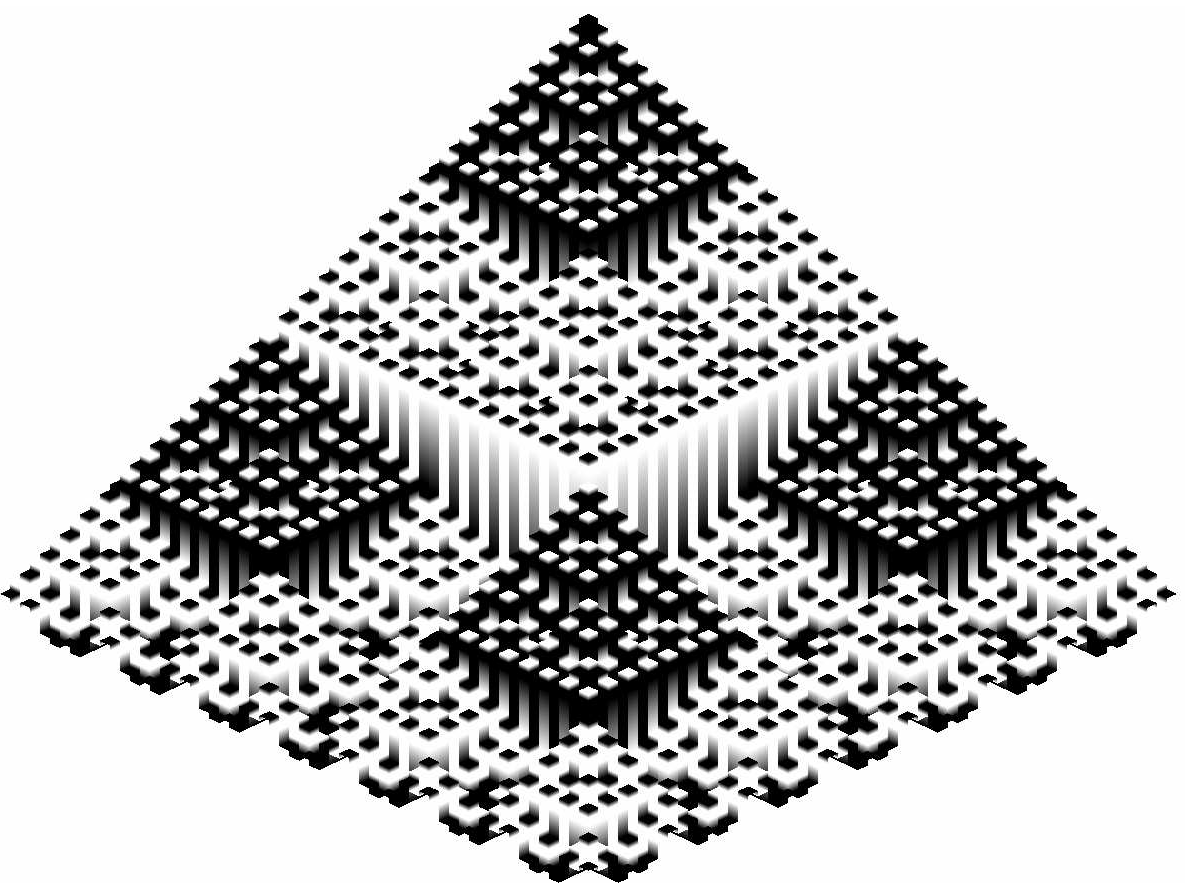
\includegraphics[width=7cm]{cheops}
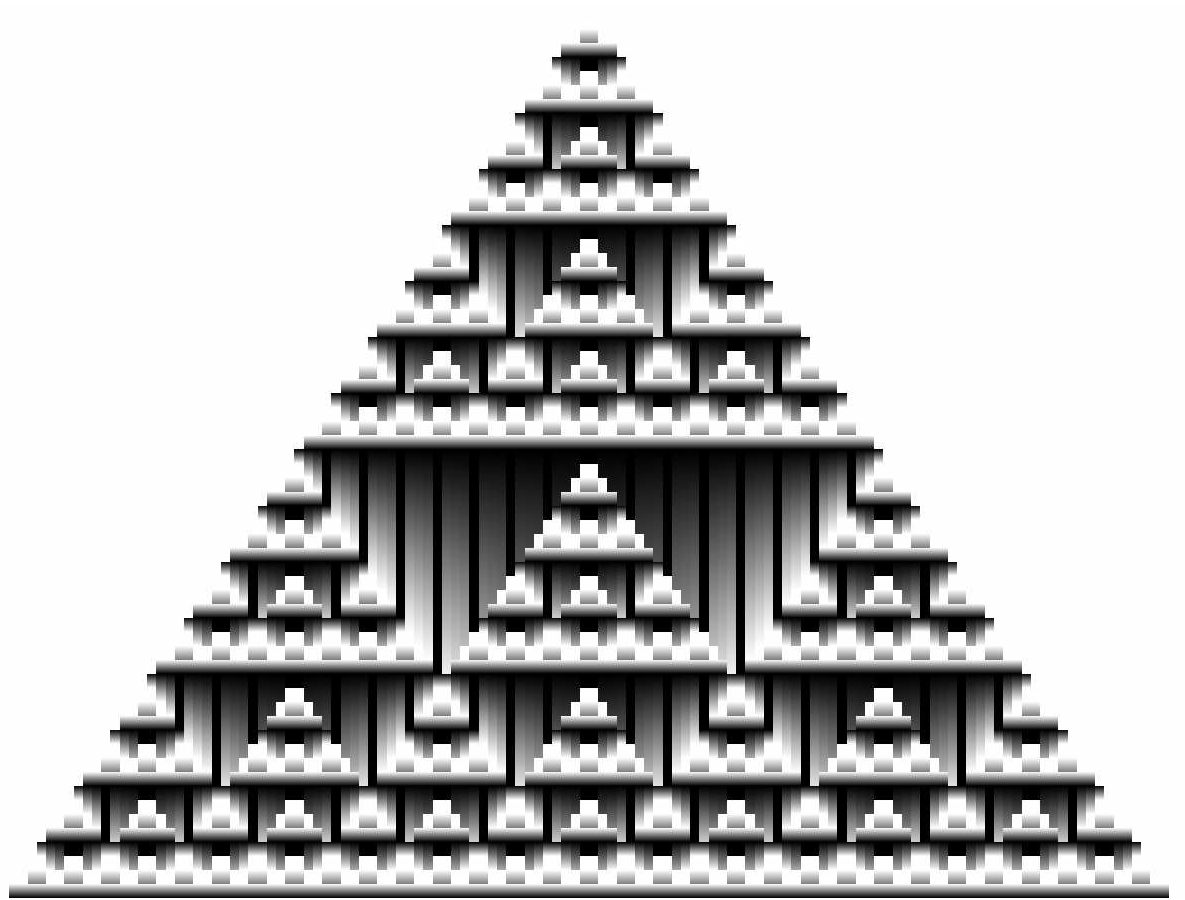
\includegraphics[width=0.5\textwidth]{chephren}
\end{llt}
\begin{figure}
\mbox{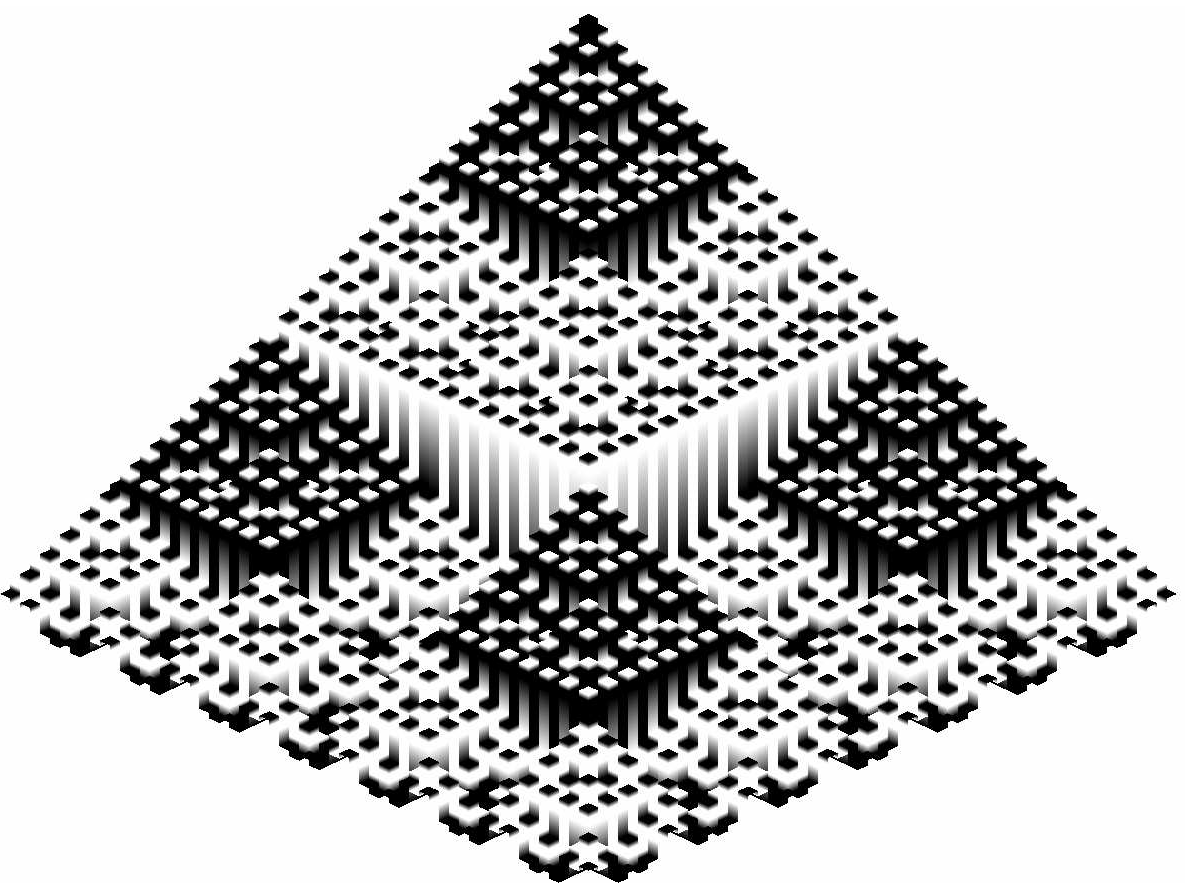
\includegraphics[width=0.5\textwidth]{cheops}}
\mbox{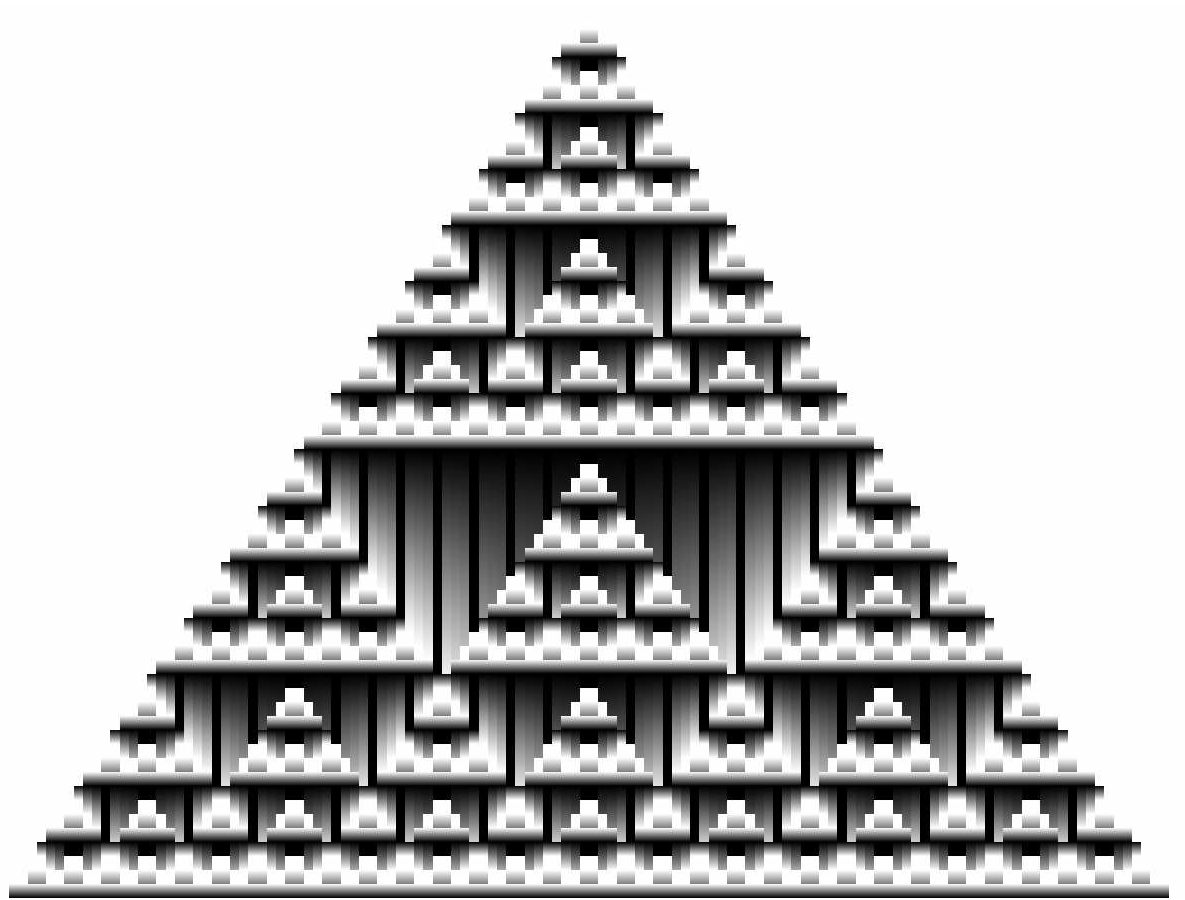
\includegraphics[width=0.5\textwidth]{chephren}}
\caption{Een figuur zegt {\scriptsize meestal} meer dan duizend woorden.}
\label{cheops-chephren}
\end{figure}
We zien dat we gebruik kunnen maken van de speciale lengte \lcommand{\\textwidth},\index{textwidth@\lcommand{\\textwidth}} die de breedte van de tekst weergeeft. De tweede figuur wordt even breed als de helft van de tekstbreedte. Het resultaat van deze commando's is te bezichtigen in figuur \ref{cheops-chephren}.
\npar
Figuren bewaren we best niet in de hoofdirectory van onze thesis. We maken bijvoorbeeld een subdirectory \bestand{figuren} aan. Zodus wordt het bovenstaande commando 
\begin{llt}
\includegraphics{figuren/figuurnaam}
\end{llt}
Niet zeer handig om altijd diezelfde directory te moeten intypen. Vandaar dat je in de \engels{preamble} kan opgeven in welke directories \latex naar figuren moet gaan zoeken:\label{graphicspath}
\begin{llt}
\graphicspath{{figuren/}{nog_een_dir_met_figuren/}}
\end{llt}
Wanneer de \latex compiler een figuur moet invoegen, gaat hij nu zoeken in de directory \bestand{figuren/} en in \bestand{nog_een_dir_met_figuren/}.
Merk op dat ook onder Windows de slash met een positieve richtingsco�ffici�nt moet gebruikt worden (en niet de \engels{backslash}).

\section{Zwevende tabellen en figuren}

\subsection{Zwevend maken}

Met de \lcommand{tabular} omgeving wordt de tabel daar geplaatst waar ze gedefinieerd werd. Met \lcommand{\\includegraphics} wordt de figuur daar geplaatst waar het commando gegeven werd. Als een tabel niet op de huidige bladzijde past, wordt een nieuwe bladzijde begonnen. Hetzelfde bij figuren. Dit kan zorgen voor nogal wat halflege bladzijden. Vandaar dat het beter is om de \latex compiler te laten beslissen waar de tabellen en figuren moeten geplaatst worden. Dit gebeurt via het zogenaamde \begrip{float} mechanisme. De tabellen en figuren worden in een \engels{float} omgeving geplaatst.
\npar
Voor tabellen wordt de \lcommandx{table} omgeving gebruikt:
\begin{llt}
\begin{table}[waar]
  \begin{tabular}{ccc}
   ... %  tabeltekst
  \end{tabular}
\end{table}
\end{llt}
Het genereren van de tabel zelf gebeurt zoals uitgelegd in sectie \ref{tabellen}.
Figuren worden in een \lcommandx{figure} omgeving geplaatst:
\begin{llt}
\begin{figure}[waar]
  \includegraphics[width=5cm]{vbfig01}
\end{figure}
\end{llt}
Op zich doen \lcommand{table} en \lcommand{figure} juist hetzelfde: ze nemen de tabel of figuur vast en zetten die op een typografisch verantwoorde plaats. Met het optionele argument (bemerk de vierkante haken) \lcommand{waar} kunnen we onze voorkeur uitdrukken over waar we de figuur graag zouden hebben. Het argument \lcommand{waar} kan uit verschillende letters bestaan. Deze letters zijn de volgende:\label{plaatsingfloat}
\begin{description}
\item[h] (Hier) De figuur of tabel mag op de plaats komen waar hij in de brontekst wordt ingegeven.
\item[t] (Top) De figuur of tabel mag aan de bovenkant van de huidige bladzijde komen, of als daar niet genoeg plaats is, aan het begin van de volgende bladzijde.
\item[b] (Beneden) De figuur of tabel mag aan de onderkant van de huidige bladzijde komen. Als daar niet genoeg plaats meer is, wordt de onderkant van de volgende bladzijde gebruikt.
\item[p] (Pagina) De figuur of tabel wordt opgespaard tot het einde van het hoofdstuk of sectie, waar een aantal bladzijden worden voorzien met alleen maar figuren en tabellen.
\item[!] Normaalgezien respecteert \latex een aantal regeltjes over de hoeveelheid \engels{floats} op een bladzijde, het aantal \engels{floats} in het begin van een pagina, en zo meer. Dit zorgt ervoor dat figuren en tabellen soms nogal ver van hun oorspronkelijke tekst geplaatst worden. Door een uitroepteken mee te geven met de positioneringsargumenten, zeggen we tegen \latex om geen rekening te houden met die typografische regels. We riskeren dan wel bladzijden te krijgen waar enkel \engels{floats} op staan.
\item[H] (Hier en nergens anders!) Soms willen we de tabel of figuur krijgen daar waar ze gedefinieerd wordt. Zelfs als daarvoor een nieuwe bladzijde moet begonnen worden. Deze optie is niet aanwezig in de standaard \latex maar moet opgeladen worden met een nieuw pakket met de originele naam \begrip{float}:
\begin{llt}
\usepackage{float}  % Om nieuwe float omgevingen aan te maken. Ook optie H!
\end{llt}
Dit pakket laat ook toe om eigen float omgevingen te maken, maar hiervoor verwijzen we naar de excellente documentatie van het pakket zelf.\footnote{Op een Debian systeem: \bestand{/usr/share/doc/texmf/latex/styles/float.dvi.gz}}
\end{description}
Dus met \lcommand{\\begin\{table\}\[ht!\] tabel \\end\{table\}} maken we een zwevende tabel die hier geplaatst wordt en als dat niet gaat, op de top van de volgende bladzijde. \latex moet zich ook niets aantrekken van typografische beperkingen in verband met \engels{floats}.

\subsection{Bijschrift}\index{bijschrift}\index{caption@\lcommand{\\caption}}

Het is altijd leuk als de lezers wat extra uitleg krijgen bij een tabel of figuur. Dit versieren gebeurt met het commando \lcommand{\\caption\{uitleg\}}. Bij de \lcommand{figure} omgeving genereert dit de titel \mbox{`Figuur 1.3: uitleg'} en bij de \lcommand{table} omgeving \mbox{`Tabel 1.3: uitleg'}. Traditioneel wordt een figuur versierd met een onderschrift en een tabel met een bovenschrift. Daarom dat bij een tabel het \lcommand{\\caption} commando wordt gegeven v��rdat de \lcommand{tabular} omgeving begint en bij een figuur n� de \lcommand{\\includegraphics}.
\npar
Standaard is het bijschrift in \latex niet echt te onderscheiden van de rest van het document (zelfde lettertype, zelfde lettergrootte, geen inspringing). Om hieraan te verhelpen, kan het pakket \lcommand{caption} gebruikt worden. Voor de uitgebreide mogelijkheden die dit pakket biedt, verwijzen we naar de uitstekende documentatie.\footnote{Op een Debian systeem: \url{/usr/share/doc/texmf/latex/caption/caption.pdf.gz}.}
\npar
Om \lcommand{caption} te gebruiken, is de volgende lijn nodig in de \engels{preamble}:
\begin{llt}
\usepackage[opties]{caption} 
\end{llt}
Hierbij zijn het \lcommand{opties} die de bijschriften van onze tabellen en figuren bepalen. De mogelijkheden zijn:
\begin{description}
\item[Stijl] De volgende argumenten kunnen gebruikt worden om te bepalen hoe het bijschrift wordt uitgelijnd.
\begin{description}
\item[normal] Volle regels worden uitgemiddeld. De laatste lijn wordt links uitgelijnd. Dit is zoals gewone tekst.
\item[flushleft] Alle regels worden tegen de linkerkantlijn geduwd.
\item[flushright]   Alle regels worden tegen de rechterkantlijn geduwd.
\item[center] Alle regels worden gecentreerd.
\item[centerlast] Alle regels worden uitgemiddeld. De laatste lijn wordt gecentreerd.
\item[hang] Hetzelfde als \lcommand{normal}, behalve dat vanaf de tweede regel van het bijschrift de tekst inspringt met een lengte gelijk aan die van de titel van het bijschrift.
\item[noonline] Al de bovenvermelde uitlijningsopties hebben alleen betrekking op bijschriften die meerdere regels tellen. Wanneer er slechts ��n regel tekst is, wordt het bijschrift gecentreerd. Om dit tegen te gaan, kan de optie \lcommand{noonline} meegegeven worden. Is niet echt aan te raden wanneer je je tabellen en figuren centreert~\ldots
\end{description}
\item[Lettergrootte] De lettergrootte voor het bijschriftlabel (`Figuur 1.3') en de bijschrifttekst kan bepaald worden door ��n van de volgende opties mee te geven: \lcommand{scriptsize}, \lcommand{footnotesize}, \lcommand{small}, \lcommand{normalsize}, \lcommand{large}, \lcommand{Large}. Uitleg over de betekenis hiervan is te vinden op bladzijde \pageref{lettergrootte}.
\item[Lettertype van het bijschriftlabel] Met de volgende opties kan het lettertype van het bijschriftlabel veranderd worden: \lcommand{sc} voor \textsc{Small Caps}, \lcommand{it} voor \textit{cursief}, \lcommand{sl} voor \textsl{slanted} en \lcommand{up} voor rechte tekst. Met \lcommand{bf} wordt het label in het vet gezet. Om \textsf{Sans Serif} als lettertype te gebruiken, kan \lcommand{sf} als optie meegegeven worden.
\end{description}
Voor dit document werd \lcommand{caption} opgeroepen met de volgende argumenten:
\begin{llt}
\usepackage[small,bf,hang]{caption}    % Om de captions wat te verbeteren
\end{llt}
Het bijschrift wordt iets kleiner afgeprint dan gewone tekst. Het label staat in het vet en vanaf de tweede lijn springt de tekst in. Als voorbeeld is er figuur \ref{mycerinus}.
\begin{figure}[ht]
\begin{center}
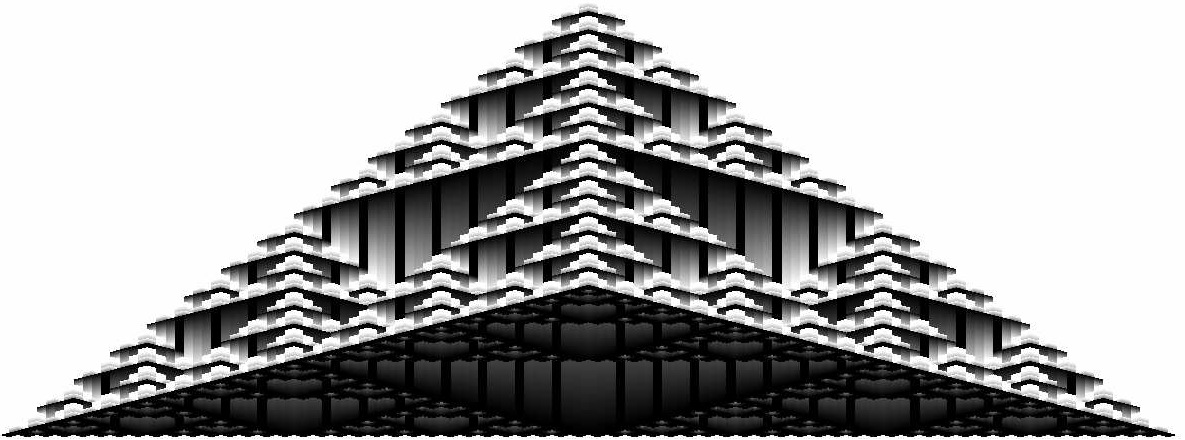
\includegraphics[width=0.9\textwidth]{mycerinus}
\caption{We hadden ook de demonstratie kunnen doen met een tabel, maar tabellen bevatten meestal slechts woorden en volgens figuur \ref{cheops-chephren} zegt een figuur meer dan duizend woorden. Dus hoewel dit bijschrift lang lijkt (nodig om dat inspringen te illustreren), is de figuur nog veel langer.\label{mycerinus}}
\end{center}
\end{figure}

\subsection{Verwijzingen naar tabellen en figuren}

Het is handig wanneer we kunnen verwijzen naar onze tabellen en figuren. Dit gebeurt met het mechanisme uitgelegd in sectie \ref{label-ref} op bladzijde \pageref{label-ref}. We plaatsen een \lcommand{\\label\{labeltjefig\}} in de \lcommand{caption}. Let erop dat dit wel degelijk in de \lcommand{caption} is en niet erbuiten. Dit is logisch: de \lcommand{caption} zorgt voor nummering van de figuur; geen \lcommand{caption}, geen nummering, geen mogelijkheid om de tabel aan te wijzen. Met \lcommand{\\ref\{labeltjefig\}} of \lcommand{\\pageref\{labeltjefig\}} kunnen we refereren naar de \engels{float}.
\npar
In wetenschappelijke teksten is het gebruikelijk dat tabellen en figuren nooit verschijnen voordat ze in de tekst vermeld worden. \latex durft dit nogal eens wel te doen. Wanneer je op het einde van een bladzijde een figuur invoegt, en je hebt er juist voor het invoeren naar verwezen, kan het zijn dat die figuur bovenaan de bladzijde geplaatst wordt, dus voordat ernaar verwezen wordt. \latex gaat dus tekst die in het bronbestand v\'o\'or de figuur staat, in het finale pdf-document n� de figuur plaatsen. Om dit te vermijden, moet de volgende lijn in de \engels{preamble} opgenomen worden:
\begin{llt}
\usepackage{flafter}        % Opdat floats niet zouden voorsteken
\end{llt}
Let er dan wel op dat je eerst naar een figuur of tabel verwijst, vooraleer ze in te brengen in de tekst.

\subsection{Enkele voorbeelden}\label{voorbeeldfloat}

Het is mooi wanneer onze tabellen en figuren gecentreerd staan. Daarom dat we de \engels{floats} in een \lcommand{center} omgeving zetten. Dat centreren moet gebeuren binnen de \engels{float} omgeving (zie voorbeeld hieronder).
\npar
De code nodig om figuur \ref{mycerinus} te genereren is:
\begin{llt}
\begin{figure}[ht]
  \begin{center}
    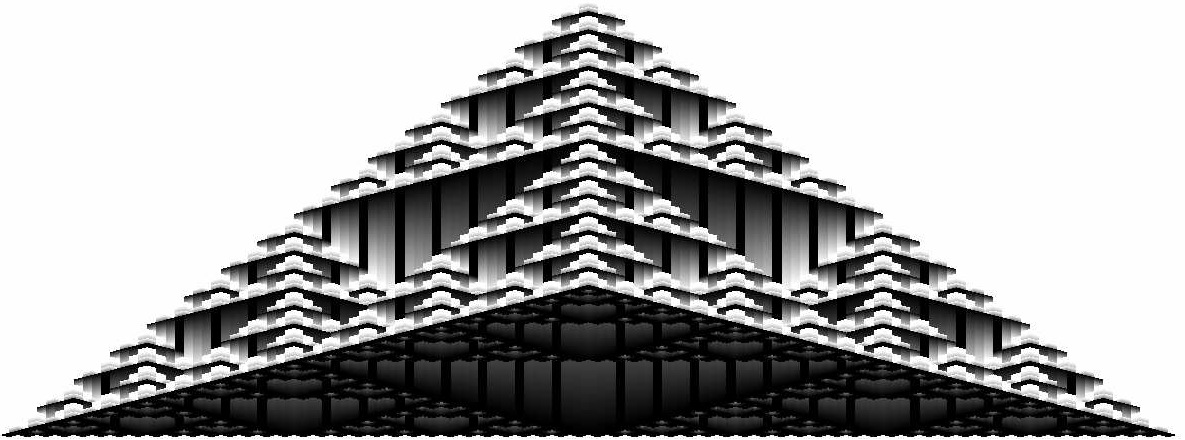
\includegraphics[width=0.9\textwidth]{mycerinus}
    \caption{We hadden ook de demonstratie kunnen doen met een tabel, maar tabellen bevatten meestal slechts woorden en volgens figuur \ref{cheops-chephren} zegt een figuur meer dan duizend woorden. Dus hoewel dit bijschrift lang lijkt (nodig om dat inspringen te illustreren), is de figuur nog veel langer.\label{mycerinus}}
  \end{center}
\end{figure}
\end{llt}
Voor tabellen gebruiken we de \lcommand{table} omgeving. In plaats van een \lcommand{\\includegraphics}, komt er nu een \lcommand{tabular} omgeving. Eventueel kunnen we de \lcommand{tabular} in een apart bestand plaatsen en in onze \lcommand{table} omgeving invoegen met een \lcommand{\\input\{tabelbestandsnaam\}} commando. Vergeet ook niet om de caption v\'o\'or de eigenlijke tabel te defini�ren. Om tabel \ref{letterstijlen} op bladzijde \pageref{letterstijlen} te genereren werd de volgende code gebruikt:
\begin{llt}
\begin{table}[h]
    \begin{center}
    \caption{Hoe verschillende letterstijlen selecteren: met een nieuwe omgeving of met een commando.\label{letterstijlen}}
        \begin{tabular}{l@{\;}l@{\quad}l@{\;}l}
        ... % de verschillende rijen
        \end{tabular}
    \end{center}
\end{table}
\end{llt}

\begin{MinderBelangrijk}
Het bijschrift even breed krijgen als de \engels{float} kan gebeuren met een \lcommand{\\parbox} (de uitleg over parboxen is te vinden op bladzijde \pageref{parbox}):
\begin{llt}
\begin{figure}[ht]
  \begin{center}
    
\includegraphics[width=0.3\textwidth]{tux}
    % De volgende witte lijn is belangrijk: anders komt caption naast figuur!

    \parbox{0.3\textwidth}{\caption{Giza is dood. Leve de Penguin!\label{tux}}}
  \end{center}
\end{figure}
\end{llt}
Het resultaat is te bewonderen in figuur \ref{tux}.
\begin{figure}[ht]
  \begin{center}
    
\includegraphics[width=0.3\textwidth]{tux}
    % De volgende witte lijn is belangrijk: anders komt caption naast figuur!

    \parbox{0.3\textwidth}{\caption{Giza is dood. Leve de Penguin!\label{tux}}}
  \end{center}
\end{figure}
\end{MinderBelangrijk}

\subsection{Nieuw commando om gemakkelijk \engels{floats} in te voegen}

Altijd dat \lcommand{\\begin\{center\}}, \lcommand{\\caption}, \lcommand{\\label} intypen is nogal vermoeiend. Algauw ga je de instellingen van de vorige figuur kopi�ren en wijzig je de figuurnaam, het label en het bijschrift. Lastig, je kan gemakkelijk fouten maken. Veel handiger is als je een commando maakt dat dat allemaal voor jou doet. Wat we eigenlijk wensen, is iets als:
\begin{llt}
\mijnfiguur[plaatsingsopties]{opties-includegraphics}{bestand}{Bijschrift}
\end{llt}
Inderdaad, het is niet echt nodig om een label mee te geven. Als we ervan uitgaan dat elke bestandsnaam geen \engels{slashes} bevat (zie bladzijde \pageref{graphicspath} over het ingeven van de directories waar \latex moet zoeken naar figuren) en uniek is, kunnen we de bestandsnaam gebruiken als label. De plaatsingsopties bepalen waar de figuur moet terechtkomen (zie bladzijde \pageref{plaatsingfloat}); dit is een optioneel argument, daar we een standaardwaarde kunnen gebruiken voor het hele document. De opties voor \lcommand{includegraphics} zijn verplicht. Meestal moet de figuur toch herschaald worden en is een \lcommand{width=xxx} nodig. Dit kan moeilijk dezelfde zijn voor elke figuur.
\npar
Het commando \lcommand{\\mijnfiguur} wordt als volgt gedefinieerd (voor uitleg over het aanmaken van nieuwe commando's verwijzen we naar sectie \ref{commandos} op bladzijde \pageref{commandos}):
\begin{llt}
\newcommand{\mijnfiguur}[4][ht]{
    \begin{figure}[#1]
        \begin{center}
            \includegraphics[#2]{#3}
            \caption{#4\label{#3}}
        \end{center}
    \end{figure}
    }
\end{llt}
Het eerste argument bevat de opties die vertellen waar onze figuur moet geplaatst worden. Standaard proberen we figuren te plaatsen waar ze gedefinieerd worden. Als dat niet lukt, hebben we ze liefst bovenaan een bladzijde. Het tweede argument bevat de opties voor \lcommand{includegraphics}. Het derde argument bevat de bestandsnaam, wat ook het label wordt, en het vierde argument bevat de tekst van het bijschrift.
\npar
Figuur \ref{mycerinus}, zou dus als volgt kunnen geplaatst worden in ons document:
\begin{llt}
\mijnfiguur{width=0.9\textwidth}{mycerinus}{We hadden ook de demonstratie...}
\end{llt}
Wat veel eleganter is dan heel die rompslomp in sectie \ref{voorbeeldfloat}.
\npar
Iets analoogs kan gedaan worden voor tabellen. Er moeten nu geen opties meer meegegeven worden met \lcommand{includegraphics} zodat we slechts drie argumenten hebben (merk ook op dat de caption v\'o\'or de tabelinput komt):
\begin{llt}
\newcommand{\mijntabel}[3][ht]{
    \begin{table}[#1]
        \begin{center}
            \caption{#3\label{#2}}
            \input{#2}
        \end{center}
    \end{table}
    }
\end{llt}
Ingeven van een tabel gebeurt dan als volgt:
\begin{llt}
\mijntabel[hb]{bestand-met-tabel}{Bijschrift bij de tabel.}
\end{llt}



\chapter{Bibliografische verwijzingen}

Het verwijzen naar literatuur is iets dat frequent gebeurt in wetenschappelijke documenten. En dat verwijzen moet volgens welbepaalde regels gebeuren, geen komma teveel of te weinig.\footnote{Wellicht is het van literatuurverwijzingen dat de term `kommaneuterij' komt} Maar er zijn leukere dingen om te doen dan te letten op punten en komma's. Laat het vervelende werk over aan de computer. Het systeem is in \latex zo opgebouwd dat je met het commando \lcommand{\\citet\{auteurkey\}} de naam van de auteur samen met het jaar krijgt en de volledige referentie achteraan in de bibliografie. Hiervoor moeten alle gebruikte referenties in een bibliografische databank zitten. In dit deel wordt kort overlopen hoe een bruikbare bibliografie kan verkregen worden voor een thesis. Voor meer opties en andere manieren van citeren (bijvoorbeeld met nummers in plaats van met auteur, jaar) verwijzen we naar de helpbestanden van \bibtex.\footnote{Op een Debian systeem in \bestand{/usr/share/doc/texmf/bibtex/base/btxdoc.dvi.gz}}

\section{\bibtex, het programma}

In feite gebeurt het genereren van de bibliografie door een extern programma, dat de bibliografische informatie uit een aantal databanken\footnote{Een duur woord voor platte tekstbestanden met speciale opmaak} haalt. Daarom dat op de plaats waar we de bibliografie wensen in te voegen, het volgende commando moet gegeven worden:
\begin{llt}
\bibliography{bibliodatabase1, bibliodatabase2, ... }
\end{llt}
De argumenten \lcommand{bibliodatabase1} en  \lcommand{bibliodatabase2}, gescheiden door komma's, zijn de bestandsnamen van de databanken zonder de extensie \bestand{.bib}. Dus de volledige naam van de databanken luidt \bestand{bibliodatabase1.bib} en \bestand{bibliodatabase2.bib}. Meerdere bestanden mogen opgegeven worden. Dit opent perspectieven voor samenwerking~\ldots
\npar
Het citeren in de tekst wordt uitgelegd in sectie \ref{cite-et-all}. Om de bibliografie effectief in het pdf document op te nemen, laten we onze tekst een eerste keer verwerken door de \latex compiler. Daarna geven we het commando:
\begin{lt}
bibtex naam-van-ons-document-zonder-extensie
\end{lt}
In TeXnicCenter (de \latex editor onder windows) is er een knopje om \bibtex op te roepen. Dit commando genereert dan twee bestanden: \bestand{ons-document.bbl} en \bestand{ons-document.blg}. Het \bestand{.blg}-bestand (van \bibtex log) is analoog aan het \latex \bestand{.log}-bestand (zie bladzijde \pageref{logbestand}) en is niet echt belangrijk. Het \bestand{.bbl}-bestand (van \bibtex BibLiografie) is te vergelijken met het \latex \bestand{.aux}-bestand en bevat informatie voor de \latex compiler om op een juiste manier de bibliografie te genereren.
\npar
Wanneer we ons document opnieuw door de \latex compiler laten verwerken (minimum twee keer, zie bladzijde \pageref{inhoudsopgave}), wordt de bibliografie in het document opgenomen.
\npar
Standaard produceert \lcommand{\\citet\{auteurkey\}} nummers in de tekst, zoals dit: [13]. Voor een thesis is het auteur--jaar mechanisme te verkiezen, zoals dit: \cite{baal01}. Hiervoor moeten we een aantal extra instructies meegeven in ons document. Vooreerst moet \lcommandx{natbib} gebruikt worden. Dit is een pakket dat de functionaliteit van \bibtex vergroot.
\begin{llt}
\usepackage[round]{natbib}         % Voor auteur-jaar citaties.
\end{llt}
Deze regel zorgt ervoor dat \lcommand{natbib} geladen wordt en ronde haakjes gebruikt. 
\begin{MinderBelangrijk}
Om de punctuaties in te stellen kan eventueel de volgende lijn in de \engels{preamble} worden opgenomen (maar de standaardwaarden zijn meestal wel goed):\index{bibpunct@\lcommand{\\bibpunct}}
\begin{llt}
\bibpunct{(}{)}{;}{y}{,}{,}  % Auteur-jaar citaties, zie natbib.dvi voor uitleg
\end{llt}
Er zijn zes argumenten, waarmee de volgende zaken kunnen aangepast worden:
\begin{enumerate}
\item Het `open de haakjes' symbool. Standaard gelijk aan \lcommand{(}.
\item Het `sluit de haakjes' symbool, Standaard gelijk aan \lcommand{)}.
\item Het punctuatiesymbool tussen verschillende citaties. Standaard is dit \lcommand{;} Dit toepassen op een voorbeeld geeft \citet{baal01,jones02}.
\item De letter \lcommand{n} voor citaties met nummers, \lcommand{s} om de nummers in superscript te zetten en alle andere letters om auteur-jaar citatie te bekomen. Dit laatste wordt standaard gebruikt.
\item Het punctuatiesymbool dat gebruikt wordt tussen de auteur en het jaar in het geval dit laatste niet tussen haakjes wordt gezet. Standaard is dit \lcommand{,} zoals in \citep{baal01}.
\item Het punctuatiesymbool dat verschijnt wanneer de auteurs van twee (of meer) artikels gelijk zijn. Door \bibtex wordt dit dan gecombineerd tot \mbox{1999a,b}. Standaard dus een komma.
\end{enumerate}
\end{MinderBelangrijk}

Doordat citeren vooral belangrijk is in wetenschappelijke literatuur en dat wetenschappelijke literatuur meestal Engelstalig is, zet \bibtex standaard \engels{and} tussen de verschillende auteurs, bv Jones and Allen (2002). Voor een Nederlandse thesis is dit geen zicht. De oplossing is om zelf een bibliografisch opmaakbestand te maken. De manier waarop \bibtex de bibliografie verwerkt zit namelijk niet in het programma zelf ingebakken, maar wordt ingelezen uit een opmaakbestand.

\begin{MinderBelangrijk}
\npar
Een nieuw \bibtex opmaakbestand maken, kan gebeuren door het speciale bestand \bestand{makebst.tex} te \LaTeX en (met \command{latex} en niet met \command{pdflatex}). Dit bestand bevindt zich normaalgezien ergens in de \latex installatie. Daar \latex ook een programmeertaal is, kan het gebruikt worden om programma's te schrijven. Dit is wat het commando \command{latex makebst.tex} doet: we krijgen een vraag-en-antwoord-dialoog waarin we puntje voor puntje kunnen kiezen hoe onze bibliografie er moet uitzien. Al deze opties worden bewaard onder de naam \bestand{bibliodutch} (die bestandsnaam is het antwoord op ��n van de eerste vragen) met standaard extensie \bestand{.dbj}. Dit is opnieuw een \latex programma (ja, ja, een programma dat een programma schrijft). Met \command{latex bibliodutch.dbj} wordt het bestand \bestand{bibliodutch.bst} gecre�erd. Dit is het bibliografisch opmaakbestand dat we nodig hebben.
\npar
\end{MinderBelangrijk}

Natuurlijk is het veel gemakkelijker om ergens zo een opmaakbestand van iemand te kopi�ren. Het opmaakbestand dat voor dit document gebruikt werd, is vrij beschikbaar~\ldots
\npar
Om dit opmaakbestand effectief te gebruiken, moet de volgende regel in de \engels{preamble} toegevoegd worden:
\begin{llt}
\bibliographystyle{bibliodutch}
\end{llt}
Verder moet het bestand \bestand{bibliodutch.bst} zich in de werkdirectory bevinden, zodat \bibtex eraan kan.
\npar
Om ervoor te zorgen dat de bibliografie in de inhoudstafel wordt opgenomen (standaard gebeurt dit namelijk niet) moet het pakket \lcommandx{tocbibbind} in de \engels{preamble} opgeladen worden:
\begin{llt}
\usepackage[nottoc]{tocbibind}	% Bibliografie in ToC; zie tocbibind.dvi
\end{llt}
De optie \lcommand{nottoc} zorgt ervoor dat de inhoudsopgave zelf niet in de inhoudsopgave komt.

\section{De bibliografische databank}

\subsection{Opbouw van de databank}\label{bibvb1}

De bibliografische databank bestaat uit verschillende items. Elk item komt overeen met ��n referentie en is van de vorm:
\begin{llt}
@article{athos:92,
    author = {A. Athos and D. Porthos and D. Aramis},
    title = {The influence of Women on society and how to cope with},
    journal = {Journal of Random Logic},
    year = {1992},
    volume = {13},
    pages = {11-19}
}
\end{llt}
Het eerste woord, vooraf gegaan door een @, bepaalt het type item dat we wensen in te voegen. In dit geval is dat een artikel. Dan worden de verschillende eigenschappen van het artikel opgegeven tussen accolades. De verschillende eigenschappen worden van elkaar gesplitst door komma's. Na de laatste eigenschap (in het voorbeeld \lcommand{pages}) staat er dus geen komma. De eerste eigenschap is de \begrip{key} van die referentie. Dit is hetgeen gebruikt wordt om in de tekst naar dat artikel te refereren (e.g. \lcommand{\\citet\{athos:92\}} geeft `\citet{athos:92}'). De rest van de eigenschappen mag in gelijk welke volgorde voorkomen.
\npar
Samengevat hebben we dus: \lcommand{@article\{key, eig1, eig2,..., eigN\}} waarbij de verschillende eigenschappen de volgende vorm hebben: \lcommand{eig1 = \{waarde\}} of \lcommand{eig1 = "waarde"} (dubbele aanhalingstekens of accolades, je mag kiezen). Verder mag elke eigenschap op een nieuwe regel geplaatst worden. Dit bevordert de overzichtelijkheid.
\npar
Meestal komen vele artikels uit hetzelfde tijdschrift. Het is lastig om dan elke keer opnieuw de volledige naam van dat tijdschrift te moeten intypen. Vandaar dat we in het begin van onze \bibtex database afkortingen mogen defini�ren. Dit gebeurt als volgt:
\begin{llt}
@string{JRL = "Journal of Random Logic"}
\end{llt}
Dit kunnen we dan als volgt gebruiken in de \bibtex items:\index{string}
\begin{llt}
...
    journal = JRL,
    year = {1992}
...
\end{llt}
Merk op dat afkortingen die gedefinieerd zijn met \lcommand{@string\{...\}} niet tussen accolades of aanhalingstekens mogen staan.
\npar
\bibtex heeft de eigenschap om in titels (het \lcommand{title} veld) alle hoofdletters om te zetten naar kleine letters. Om dit tegen te gaan (voor namen bijvoorbeeld), moeten de letters nog eens extra tussen accolades gezet worden. Dus 
\begin{llt}
...
    title = {The influence of {Women} on society and how to cope with},
...
\end{llt}
zorgt ervoor dat Women met een hoofdletter blijft staan in de bibliografie van ons finaal \bestand{pdf}-document. Verder mogen allerhande \latex opmaak commando's gebruikt worden in de bibliografie:

\begin{llt}
...
    title = {The relation of \textit{E. coli} to humankind},
...
\end{llt}
Het is aangeraden om accenten en andere specialiteiten tussen accolades te zetten, dus \lcommand{\{\\"o\}} en niet \lcommand{\\"o} om ergens in de bibliografie \"o te produceren.


\subsection{De verschillende items}

Zoals in de vorige sectie werd beschreven, begint elk \bibtex item met een @ gevolgd door de naam van het documenttype waarnaar het item verwijst (boek, artikel,\ldots). Afhankelijk van wat het item is, kunnen verschillende eigenschappen gegeven worden. Niet elke eigenschap kan bij elk item gegeven worden. Het is bijvoorbeeld niet mogelijk om de \engels{journal} mee te geven bij een boek. Een \engels{journal} past meer bij een artikel. Verder zijn sommige velden verplicht, en andere optioneel. Bij een artikel moet bijvoorbeeld altijd de auteur gegeven worden, maar niet het tijdschriftnummer. De verschillende velden worden beschreven in de volgende sectie. Hier geven we een overzicht van de mogelijke items. Diegenen die dieper op het onderwerp willen ingaan, worden doorverwezen naar \bestand{btxdoc.dvi}.
\newcommand{\bibent}[4]{\item[@]\lcommandx{#1}\hspace{\labelsepp}#2\\
    \mbox{}\quad\parbox{0.15\textwidth}{Verplicht:}\parbox[t]{0.76\textwidth}{#3}\\
    \mbox{}\quad\parbox{0.15\textwidth}{Optioneel:}\parbox[t]{0.76\textwidth}{\renewcommand{\baselinestretch}{1}\small\normalsize #4}
    }
\begin{itemize}
\newlength{\labelsepp}
\setlength{\labelsepp}{\labelsep}
\setlength{\labelsep}{0pt}
\bibent{article}{Om een artikel op te nemen.}{\lcommand{author}, \lcommand{title}, \lcommand{journal}, \lcommand{year}.}{\lcommand{vol}, \lcommand{number}, \lcommand{pages}, \lcommand{month}, \lcommand{note}.}
\bibent{book}{Een boek met een expliciete uitgever.}{\lcommand{author} of \lcommand{editor}, \lcommand{title}, \lcommand{publisher}, \lcommand{year}.}{\lcommand{volume} of \lcommand{number}, \lcommand{series}, \lcommand{address}, \lcommand{edition}, \lcommand{month}, \lcommand{note}.}
\bibent{booklet}{Een boek zonder auteur of uitgever.}{\lcommand{title}.}{\lcommand{author}, \lcommand{howpublished}, \lcommand{address}, \lcommand{month}, \lcommand{year}, \lcommand{note}.}
\bibent{inbook}{Een deel van een boek (hoofdstuk, sectie).}{\lcommand{author} of \lcommand{editor}, \lcommand{title}, \lcommand{chapter} en/of \lcommand{pages}, \lcommand{publisher}, \lcommand{year}.}{\lcommand{volume} or \lcommand{number}, \lcommand{series}, \lcommand{type}, \lcommand{address}, \lcommand{edition}, \lcommand{month}, \lcommand{note}.}
\bibent{incollection}{Een deel van een boek met een eigen titel.}{\lcommand{author}, \lcommand{title}, \lcommand{booktitle}, \lcommand{publisher}, \lcommand{year}.}{\lcommand{editor}, \lcommand{volume} of \lcommand{number}, \lcommand{series}, \lcommand{type}, \lcommand{chapter}, \lcommand{pages}, \lcommand{address}, \lcommand{edition}, \lcommand{month}, \lcommand{note}.}
\bibent{inproceedings}{Een artikel in de \engels{proceedings} van een conferentie.}{\lcommand{author}, \lcommand{title}, \lcommand{booktitle}, \lcommand{year}.}{\lcommand{editor}, \lcommand{volume} of \lcommand{number}, \lcommand{series}, \lcommand{pages}, \lcommand{address}, \lcommand{month}, \lcommand{organization}, \lcommand{publisher}, \lcommand{note}.}
\bibent{manual}{Voor technische documentatie zoals gebruiksaanwijzingen.}{\lcommand{title}.}{\lcommand{author}, \lcommand{organization}, \lcommand{address}, \lcommand{edition}, \lcommand{month}, \lcommand{year}, \lcommand{note}.}
\bibent{masterthesis}{Voor een afstudeerthesis.}{\lcommand{author}, \lcommand{title}, \lcommand{school}, \lcommand{year}.}{\lcommand{type}, \lcommand{address}, \lcommand{month}, \lcommand{note}.}
\bibent{misc}{De vuilbak, als de rest niet past.}{Geen.}{\lcommand{author}, \lcommand{title}, \lcommand{howpublished}, \lcommand{month}, \lcommand{year}, \lcommand{note}.}
\bibent{phdthesis}{Voor een doctoraatsthesis. Eigenlijk hetzelfde als een afstudeerthesis~\ldots}{\lcommand{author}, \lcommand{title}, \lcommand{school}, \lcommand{year}.}{\lcommand{type}, \lcommand{address}, \lcommand{month}, \lcommand{note}.}
\bibent{proceedings}{Een publicatie voortvloeiend uit een conferentie.}{\lcommand{title}, \lcommand{year}.}{\lcommand{editor}, \lcommand{volume} of \lcommand{number}, \lcommand{series}, \lcommand{address}, \lcommand{month}, \lcommand{organization}, \lcommand{publisher}, \lcommand{note}.}
\bibent{techreport}{Voor een technisch of intern rapport.}{\lcommand{author}, \lcommand{title}, \lcommand{institution}, \lcommand{year}.}{\lcommand{type}, \lcommand{number}, \lcommand{address}, \lcommand{month}, \lcommand{note}.}
\bibent{unpublished}{Voor ongepubliceerd werk met titel en auteur.}{\lcommand{author}, \lcommand{title}, \lcommand{note}.}{\lcommand{month}, \lcommand{year}.}
\end{itemize}
Laat je niet afschrikken door dit overweldigend aanbod aan mogelijkheden. De meest gebruikte items zijn \lcommand{article} en soms nog \lcommand{book}. De rest is voor speciale literatuur. Verder moet de benaming gezien worden als hulpmiddel om te onthouden welke mogelijkheden er bestaan, maar moet dit niet strikt opgevolgd worden. Je mag zeker \lcommand{masterthesis} gebruiken voor een \mbox{Ph.D} thesis. Beide items geven juist hetzelfde resultaat.

\subsection{De verschillende eigenschappen}

De verschillende eigenschappen die in de items kunnen ingevuld worden, zijn:
\renewcommand{\bibent}[2]{\item[]\mbox{}\hspace{-\leftmargin}\lcommandx{#1}\hspace{\labelsepp}#2}
\begin{itemize}
\setlength{\labelsepp}{\labelsep}
\setlength{\labelsep}{0pt}
\bibent{address}{Het adres van de uitgever.}
\bibent{author}{De auteurs.}
\bibent{booktitle}{De titel van het boek, wanneer slechts een deel van dat boek geciteerd wordt.}
\bibent{chapter}{Een hoofdstuk of sectienummer.}
\bibent{edition}{De editie van het boek. Bijvoorbeeld `Derde'. Het woordje `editie' moet er niet achter komen, daar zorgt \bibtex voor.}
\bibent{editor}{De uitgever van het boek, niet te verwarren met de auteur.}
\bibent{howpublished}{Hierin kunnen allerhande speciale mededelingen gestoken worden, bijvoorbeeld `Persoonlijke mededeling'.}
\bibent{institution}{In een technisch rapport komt hier de naam van de financierder.}
\bibent{journal}{De naam van het tijdschrift waaruit een artikel komt.}
\bibent{month}{De maand in dewelke het werk geschreven werd. Wordt zelden gebruikt.}
\bibent{note}{Extra informatie die toegevoegd moet worden aan de bibliografie. Moet beginnen met een hoofdletter.}
\bibent{number}{Het nummer van een tijdschrift of een ander werk dat in series wordt uitgegeven. Wetenschappelijke tijdschriften hebben meestal een volume en een nummer. De bladzijdetelling loopt meestal door in de verschillende nummers van eenzelfde volume. Zodus is het niet nodig om ook het nummer van een tijdschrift mee te geven in de bibliografie.}
\bibent{organization}{De sponsor van de conferentie.}
\bibent{pages}{De bladzijden bestreken door het werk. Voor tijdschriften is het gebruikelijk om een bereik mee te geven: \lcommand{99-102}.}
\bibent{publisher}{De naam van de uitgever.}
\bibent{school}{De naam van de instelling waar de thesis geschreven werd.}
\bibent{series}{De naam van de serie. De titel bevat dan de naam van het boek zelf.}
\bibent{title}{Titel van het werk.}
\bibent{type}{Het type werk, bijvoorbeeld `Beleidsnota'.}
\bibent{volume}{Het volumenummer van een tijdschrift. Is niet verplicht maar sterk aangeraden.}
\bibent{year}{Het jaar van publicatie.}
\end{itemize}
Ook hier moet men zich niet te streng houden aan de benaming. In het auteursveld mag zeker `Anonymous' staan.

\subsubsection*{Iets meer over het veld \lcommand{author}}\index{author}

Elke auteur wordt gescheiden door het woordje \lcommandx{and}. Een auteur kan ingegeven worden als \lcommand{voornaam achternaam} of als \lcommand{achternaam, voornaam}. Dit heeft geen invloed op hoe de auteurs geciteerd worden in de bibliografie. \bibtex wisselt die volgorde om, afhankelijk van de gebruikte citatiestijl. Bij de eerste mogelijkheid \lcommand{voornaam achternaam} kan het gebeuren dat delen van samengestelde namen niet meegenomen worden in de achternaam. Bij de tweede manier weet \bibtex met zekerheid wat de voornaam is en wat de achternaam (de twee worden namelijk gescheiden door een komma). Het voorbeeld van sectie \ref{bibvb1} zou dus beter als volgt geschreven worden:
\begin{llt}
...
    author = {Athos, A. and Porthos, D. and Aramis, D.},
...
\end{llt}

\subsection{Templates}

Het is niet leuk om telkens opnieuw al die types en eigenschappen in te typen. Vandaar dat we met \engels{templates} kunnen werken. Dit zijn lege bibitems. Alle tekst in een \bibtex databank die niet in een item zit, wordt beschouwd als commentaar (in een item zelf kan geen commentaar ingebracht worden\footnote{Hoewel. Aangezien \bibtex alle eigenschappen negeert die het niet nodig acht voor een bepaalde item, kunnen wij de eigenschap \lcommand{commentaar = Mijn opmerkingen} toevoegen, zonder dat deze verschijnt in de bibliografie.}). Bijgevolg laten we de \engels{templates} niet starten door een @ maar bijvoorbeeld wel door een \lcommand{A}. Wanneer we een nieuw item willen toevoegen aan onze databank, kopi�ren en plakken we de lege \engels{template}, vervangen de \lcommand{A} door een @ en vullen we de verschillende items aan. Om de optionele velden te onderscheiden van de verplichte, worden ze ingesprongen. Een optioneel argument mogen we leeg laten. Als voorbeeld voor een \lcommand{article} hebben we de volgende \engels{template}:
\begin{llt}
Aarticle{,
author = {},
title = {},
journal = {},
year = {},
	volume = {},
	number = {},
	pages = {},
	note = {}
}
\end{llt}
Merk op dat de laatste eigenschap \lcommand{note} geen komma op het einde heeft. Denk hieraan wanneer je dit weinig gebruikte veld uit je items verwijdert. De komma van het vorige veld (in casu \lcommand{pages}) moet dan ook verdwijnen.
\npar
\begin{MinderBelangrijk}
Voor mensen die echt niet graag in tekstbestanden rommelen en alles liever met knopjes besturen, bestaan er programma's om je \bibtex databank te beheren. Een goed programma dat op alle besturingssystemen werkt, is JabRef: \url{http://jabref.sourceforge.net/}. Voor de Mac fanaten is er BibDesk: \url{http://bibdesk.sourceforge.net/}.
\end{MinderBelangrijk}

\section{Citeren in de tekst}\index{citet@\lcommand{\\citet}}\index{citep@\lcommand{\\citep}}\label{cite-et-all}

We hebben nu alles gezien om een bibliografie te maken, behalve het citeren in de tekst zelf. Hiervoor bestaan verschillende commando's. De twee basiscommando's zijn 
\begin{itemize}
\item \lcommand{\\citet\{athos:92\}} (CITE in Text) om te citeren in doorlopende tekst. Voorbeeld: volgens \citet{athos:92} moet je met gevaar leren leven. 
\item \lcommand{\\citep\{athos:92\}} (CITE in Parentheses) om het geciteerde werk tussen haakjes te zetten. Voorbeeld: Leve de koning \citep{athos:92}!
\end{itemize}
Deze commando's hebben ook een stervorm om alle namen te laten zien: \lcommand{\\citet*\{athos:92\}} geeft \citet*{athos:92}. Meerdere items kunnen in ��n enkel commando samengebracht worden: \lcommand{\\citep\{jones02,athos:92\}} geeft \citep{jones02,athos:92}.
\npar
Je kan ook commentaar kwijt in citaties, wat handig is wanneer de haakjes automatisch worden geplaatst:
\begin{center}
\begin{tabular}{l@{\quad\ensuremath{\longrightarrow}\quad}l}
\lcommand{\\citet\[Hoofdstuk 13\]\{athos:92\}}                  &\citet[Hoofdstuk 13]{athos:92}         \\
\lcommand{\\citep\[sectie 3\]\{jones02\}}                       &\citep[sectie 3]{jones02}              \\
\lcommand{\\citep\[in\]\[sectie 3\]\{jones02\}}                 &\citep[in][sectie 3]{jones02}          \\
\lcommand{\\citep\[in\]\[\]\{jones02\}}                         &\citep[in][]{jones02}                  
\end{tabular}
\end{center}
Wanneer haakjes ongewenst zijn, kunnen we gebruik maken van de ALternatieve commando's (\lcommand{citeal}, met de \lcommand{t} of \lcommand{p} erachter, afhankelijk of we in de tekst citeren of tussen haakjes):
\begin{center}
\begin{tabular}{l@{\quad\ensuremath{\longrightarrow}\quad}l}
\lcommand{\\citealt\{athos:92\}}                                &\citealt{athos:92}                     \\
\lcommand{\\citealt*\{athos:92\}}                               &\citealt*{athos:92}                    \\
\lcommand{\\citealp\{athos:92\}}                                &\citealp{athos:92}                     \\
\lcommand{\\citealp*\[in\]\[sectie 3\]\{jones02\}}              &\citealp*[in][sectie 3]{jones02}       \\
\end{tabular}
\end{center}
Soms wens je alleen de auteur of alleen het jaar. Dit laat toe om iets gevari�erder te citeren:
\begin{center}
\begin{tabular}{l@{\quad\ensuremath{\longrightarrow}\quad}l}
\lcommand{\\citeauthor\{athos:92\}}                             &\citeauthor{athos:92}                  \\
\lcommand{\\citeauthor*\{athos:92\}}                            &\citeauthor*{athos:92}                 \\
\lcommand{\\citeyear\{athos:92\}}                               &\citeyear{athos:92}                    \\
\lcommand{\\citeyearpar\{jones02\}}                             &\citeyearpar{jones02}                  \\
\lcommand{\\citeyearpar\[in\]\[sectie 3\]\{jones02\}}           &\citeyearpar[in][sectie 3]{jones02}    \\
\end{tabular}
\end{center}
Om in het begin van een zin een auteur te citeren wiens familienaam begint met een kleine letter, kan je gebruik maken van de hoofdlettervariant van de hierboven vermelde commando's: \lcommand{\\citet\{vanOostrum96\}} geeft: \citet{vanOostrum96}, terwijl \lcommand{\\Citet\{vanOostrum96\}} \Citet{vanOostrum96} geeft.
\npar
Artikels die nooit geciteerd worden in de tekst, komen normaalgezien ook niet voor in de bibliografie. Indien we toch ongeciteerde artikels in de bibliografie wensen op te nemen, gebruiken we het commando \lcommand{\\nocite\{key\}} om het artikel met \lcommand{key} op te nemen in de bibliografie. Met \lcommand{\\nocite\{*\}} worden alle artikels uit de bibiografische databank in de bibliografie opgenomen.




\chapter{Wiskundige formules}\label{math-mode}

Wiskundige formules in een tekst inbrengen was voor het \TeX\ tijdperk tijdrovend en dus duur. Dit is ��n van de hoofdredenen waarom Donald Knuth \TeX\ ontwikkelde. Dit is ook de reden waarom wiskundige formules tussen dollartekens staan (niet altijd echter, zie verder).
\npar
De mathematische mogelijkheden van \latex worden sterk uitgebreid door gebruik te maken van het \lcommandx{amsmath} pakket (\engels{American Mathematical Society}):
\begin{llt}
\usepackage{amsmath}     % Uitgebreide wiskundige mogelijkheden
\end{llt}
In dit hoofdstuk zullen we ervan uitgaan dat dit standaard gebruikt wordt. Sommige voorbeelden zullen anders niet werken. Verder leggen we hier niet alles uit, verre van. Voor meer exotische dingen kan onder andere de help bij het \lcommand{amsmath} pakket gebruikt worden.\footnote{Op een Debian systeem: \bestand{/usr/share/doc/texmf/latex/amsmath/amsldoc.dvi.gz}}

\section{Wiskundige omgeving}

Wiskundige formules kunnen op twee manieren ingebracht worden. Enerzijds in de tekst, zoals $E = mc^2$ en anderzijds op een aparte lijn, zoals:
\begin{equation}
    F(x) = \frac{1}{\sigma \sqrt{2\pi}}  e^{\frac{-(x-\mu)^2}{2\sigma^2}}
    \label{gauss}
\end{equation}
Wiskunde inbrengen in de tekst, gebeurt door de formule tussen dollartekens te zetten: \lcommand{$E = mc^2$}.\footnote{Ook \lcommand{\\begin\{math\} E = mc^2 \\end\{math\}} en \lcommand{\\(E = mc^2\\)} mogen gebruikt worden.} Om de formules op een aparte lijn te krijgen:
\begin{llt}
\begin{equation}
    F(x) = \frac{1}{\sigma \sqrt{2\pi}}  e^{\frac{-(x-\mu)^2}{2\sigma^2}}
    \label{gauss} % Om te kunnen refereren naar deze vergelijking
\end{equation}
\end{llt}
In plaats van \lcommandx{equation} mag ook \lcommand{equation*}\footnote{Of \lcommand{\\begin\{displaymath\} formule \\end\{displaymath\}} of \lcommand{$$ formule $$} of \lcommand{\\\[ formule \\\]}.} gebruikt worden. Deze laatste vorm vermijdt dat de vergelijkingen genummerd worden. In dit geval is het onzinnig om een label mee te geven. In een \lcommand{equation} omgeving, wordt met het labelcommando het nummer van de vergelijking in een label gezet. Bijgevolg produceert \lcommand{\\ref\{gauss\}} het nummer van vergelijking \ref{gauss}.

\subsection{Lange formules: \lcommand{multline}}

In de \lcommand{equation} omgeving, worden lijnen nooit afgebroken. \latex kan en wil niet op eigen houtje beslissen op welke plaats een formule moet gesplitst worden. Er bestaat echter een speciale omgeving in dewelke je een formule over verschillende lijnen kan uitsmeren. Dit is de \lcommandx{multline} omgeving (en dus niet \lcommand{multIline}!):
\begin{llt}
\begin{multline}
    (x+y+z)^4 = z^4 + 4 y z^3 + 4 x z^3 + 6 y^2 z^2 + 12 x y z^2 + \\
        6 x^2 z^2 + 4 y^3 z + 12 x y^2 z + 12 x^2 y z + 4 x^3 z +  \\
        y^4 + 4 x y^3 + 6 x^2 y^2 + 4 x^3 y + x^4
\end{multline}
\end{llt}
\begin{multline}
    (x+y+z)^4 = z^4 + 4 y z^3 + 4 x z^3 + 6 y^2 z^2 + 12 x y z^2 + \\
        6 x^2 z^2 + 4 y^3 z + 12 x y^2 z + 12 x^2 y z + 4 x^3 z +  \\
        y^4 + 4 x y^3 + 6 x^2 y^2 + 4 x^3 y + x^4
\end{multline}
Een nieuwe lijn beginnen gebeurt met \lcommand{\\\\}. De eerste lijn wordt links uitgelijnd, de volgende lijnen worden gecentreerd en de laatste lijn wordt rechts uitgelijnd. Het vergelijkingsnummer wordt rechts tegen de laatste lijn geplaatst. Indien geen vergelijkingsnummer gewenst is, kan \lcommand{multline*} gebruikt worden.

\begin{MinderBelangrijk}

\subsection{Meerdere formules tegelijkertijd: \lcommand{gather}, \lcommand{align}, \lcommand{eqnarray}, \lcommand{array}}

Meerdere deelvergelijkingen in ��n vergelijking kan bekomen worden met de \lcommandx{gather} omgeving:
\begin{llt}
\begin{gather}
    (a + b)^2 = a^2 + 2 a b + b^2               \label{gather1}  \\
    (a + b)^3 = a^3 + 3 a^2 b + 3 a b^2 + b^3   \nonumber        \\
    (a + b)(a - b) = a^2 - b^2                  \label{gather2}
\end{gather}
\end{llt}
\begin{gather}
(a + b)^2 = a^2 + 2 a b + b^2               \label{gather1}  \\
(a + b)^3 = a^3 + 3 a^2 b + 3 a b^2 + b^3   \nonumber        \\
(a + b)(a - b) = a^2 - b^2                  \label{gather2}
\end{gather}
De verschillende lijnen worden gecentreerd en elke lijn krijgt een vergelijkingsnummer. Er kan dus een label toegekend worden aan elke lijn. Wanneer het niet gewenst is om aan een bepaalde lijn een vergelijkingsnummer toe te kennen, kan het commando \lcommand{\\nonumber} gegeven worden.\index{nonumber@\lcommand{\\nonumber}} Dit is hetgeen gebeurde tussen vergelijking \ref{gather1} en \ref{gather2}.
\npar
Het hierboven gegeven voorbeeld zou mooier zijn, moesten de verschillende gelijkheidstekens onder elkaar staan. Hiervoor is de \lcommandx{align} omgeving zeer geschikt. Het gebruik is analoog aan een \lcommand{tabular} omgeving (bladzijde \pageref{tabular}), alleen hoeft de uitlijningsformattering van de kolommen niet meegegeven te worden: de eerste kolom wordt rechts uitgelijnd, de tweede kolom links, de derde opnieuw rechts, de vierde weer links, enzovoort. Elke rij moet hetzelfde aantal kolommen bevatten. Het wordt gebruikt om verschillende kleine vergelijkingen naast elkaar te plaatsen.
\begin{llt}
\begin{align}
    1+0 & = 1   & 1+1   & = 2   & 2+1   & = 3   & 3+1   & = 4   \label{pascal2} \\
    1+0 & = 1   & 1+2   & = 3   & 3+3   & = 6   & 6+4   & = 10  \nonumber       \\
    1+0 & = 1   & 1+3   & = 4   & 4+6   & = 10  & 10+10 & = 20  \label{pascal4}
\end{align}
\end{llt}
\begin{align}
    1+0 & = 1   & 1+1   & = 2   & 2+1   & = 3   & 3+1   & = 4   \label{pascal2} \\
    1+0 & = 1   & 1+2   & = 3   & 3+3   & = 6   & 6+4   & = 10  \nonumber       \\
    1+0 & = 1   & 1+3   & = 4   & 4+6   & = 10  & 10+10 & = 20  \label{pascal4}
\end{align}
Door het commando \lcommand{\\nonumber} te geven op het einde van een lijn, wordt die lijn niet genummerd. Wanneer we geen enkele lijn wensen te nummeren, kunnen we \lcommand{align*} gebruiken. 
\npar
De \lcommand{align} omgeving doet veel moeite om de verschillende kolommenparen mooi te spatieren. Met \lcommand{alignat}, kunnen we die spati�ring teniet doen. Alle kolommen worden dan tegen elkaar geplakt. De syntax is \lcommand{\\begin\{alignat\}\{N\}} waarbij \lcommand{N} het aantal kolomkoppels is. Met de \lcommand{flalign} omgeving worden de kolomkoppels zo ver mogelijk uit elkaar gezet, zodat heel de breedte van de bladzijde gevuld is.
\npar
Om een bepaald symbool in een vergelijking telkens op dezelfde plaats te krijgen, kan de \lcommandx{eqnarray} omgeving gebruikt worden. In die omgeving bestaat elke lijn uit drie delen: het eerste deel wordt rechts uitgelijnd, het tweede deel wordt gecentreerd en het derde deel wordt links uitgelijnd. Elke lijn krijgt een vergelijkingsnummer, tenzij het commando \lcommand{\\nonumber} wordt gegeven.
\begin{llt}
\begin{eqnarray}
(a + b)^2       & = &  a^2 + 2 a b + b^2               \label{eqnarray1}  \\
(a + b)^3       & = &  a^3 + 3 a^2 b + 3 a b^2 + b^3   \nonumber          \\
(a + b)(a - b)  & = &  a^2 - b^2                       \label{eqnarray2}  \\
                & = &  - b^2 + a^2                     \label{eqnarray3}
\end{eqnarray}
\end{llt}
\begin{eqnarray}
(a + b)^2       & = &  a^2 + 2 a b + b^2               \label{eqnarray1}  \\
(a + b)^3       & = &  a^3 + 3 a^2 b + 3 a b^2 + b^3   \nonumber          \\
(a + b)(a - b)  & = &  a^2 - b^2                       \label{eqnarray2}  \\
                & = &  - b^2 + a^2                     \label{eqnarray3}
\end{eqnarray}
Merk op dat het, zoals in de \lcommand{tabular} omgeving, ook hier mogelijk is om cellen leeg te laten, wat gebeurde in vergelijking \ref{eqnarray3}.

\subsection{Subnummering van vergelijkingen}

Om vergelijkingen die bij elkaar horen hetzelfde hoofdnummer te geven, maar verschillende subnummers, kan gebruik gemaakt worden van de \lcommandx{subequations} omgeving. Deze omgeving is eigenlijk een superomgeving, die rond alle andere wiskundige omgevingen kan geplaatst worden. Alle vergelijkingen die binnen die superomgeving worden ingegeven, krijgen hetzelfde hoofdnummer, maar verschillen in het subnummer. Het \lcommand{\\label} commando juist na \lcommand{\\begin\{subequations\}} geeft een label met alleen de hoofdnummering. De subnummering in labels steken, gebeurt door het \lcommand{\\label} commando te geven in de verschillende vergelijkingen.
\begin{llt}
\begin{subequations}
    \label{subvgl}
    \begin{equation}
        (a + b)^2      =   a^2 + 2 a b + b^2             \label{subvgl1}
    \end{equation}
    Tussen de verschillende vergelijkingen mag tekst geplaatst worden. 
    \begin{gather}
        (a + b)^3      =   a^3 + 3 a^2 b + 3 a b^2 + b^3 \label{subvgl2}   \\
        (a + b)(a - b) = a^2 - b^2                       \label{subvgl3}
    \end{gather}
\end{subequations}
\end{llt}
\begin{subequations}
    \label{subvgl}
    \begin{equation}
        (a + b)^2      =   a^2 + 2 a b + b^2             \label{subvgl1}
    \end{equation}
    Tussen de verschillende vergelijkingen mag tekst geplaatst worden. 
    \begin{gather}
        (a + b)^3      =   a^3 + 3 a^2 b + 3 a b^2 + b^3 \label{subvgl2}   \\
        (a + b)(a - b) = a^2 - b^2                       \label{subvgl3}
    \end{gather}
\end{subequations}
Het algemene nummer van de drie bovenstaande vergelijkingen is \ref{subvgl}, verkregen met het commando \lcommand{\\ref\{subvgl\}}. De individuele vergelijkingen zijn \ref{subvgl1}, \ref{subvgl2} en \ref{subvgl3}. Dit wordt verkregen met \lcommand{\\ref\{subvgl1\}}, \lcommand{\\ref\{subvgl2\}} en \lcommand{\\ref\{subvgl3\}}.

\subsection{Omgevingen binnen de \lcommand{equation} omgeving}

Om ingewikkelde constructies te maken binnen wiskundige omgevingen, kunnen subomgevingen gebruikt worden. Er zijn er vijf: \lcommandx{aligned}, \lcommandx{gathered}, \lcommand{split}, \lcommand{array} en \lcommand{cases}. Zij nummeren de vergelijking niet. Dat nummeren gebeurt door de buitenste wiskundige omgeving (in het voorbeeld hieronder \lcommand{equation}). 
\npar
De eerste twee hebben de volgende syntax:
\begin{llt}
\begin{aligned}[positie] vgl-lijnen \end{aligned}
\begin{gathered}[positie] vgl-lijnen \end{gathered}
\end{llt}
Hierbij is \lcommand{positie} een optioneel positioneringsargument dat \lcommand{b} (\engels{bottom}), \lcommand{t} (\engels{top}) of \lcommand{c} (\engels{center}, standaard) is. Het gebruik is analoog als bij \lcommand{align} en \lcommand{gather}:
\begin{llt}
\begin{equation}
    \begin{aligned}[c]
        a     &= b+c   \\   a-b   &= c   \\   a-b-c &= 0   \\
    \end{aligned}
        \quad \leftarrow\text{center---top}\rightarrow \quad
    \begin{gathered}[t]
        a      = b+c   \\   a-b    = c   \\   a-b-c  = 0   \\
    \end{gathered}
        \quad \leftarrow\text{top---bottom}\rightarrow \quad
    \begin{aligned}[b]
        a      = b+c   \\   a-b    = c   \\   a-b-c  = 0   \\
    \end{aligned}
\end{equation}
\end{llt}
\begin{equation}
    \begin{aligned}[c]
        a     &= b+c   \\   a-b   &= c   \\   a-b-c &= 0   \\
    \end{aligned}
        \quad \leftarrow\text{center---top}\rightarrow \quad
    \begin{gathered}[t]
        a      = b+c   \\   a-b    = c   \\   a-b-c  = 0   \\
    \end{gathered}
        \quad \leftarrow\text{top---bottom}\rightarrow \quad
    \begin{aligned}[b]
        a      = b+c   \\   a-b    = c   \\   a-b-c  = 0   \\
    \end{aligned}
\end{equation}
De \lcommandx{split} omgeving moet ook binnen een wiskundige omgeving voorkomen en wordt gebruikt om vergelijkingen te splitsen. Het verschil met de \lcommand{multline} omgeving is dat er in elke lijn een uitlijningsteken voorkomt \lcommand{&} zodat de schrijver meer controle heeft over hoe de vergelijkingen eruit zien.
\begin{llt}
\begin{equation}
    \begin{split}
        (x+y+z)^4 = & z^4 + 4 y z^3 + 4 x z^3 + 6 y^2 z^2 + 12 x y z^2 +     \\
                & 6 x^2 z^2 + 4 y^3 z + 12 x y^2 z + 12 x^2 y z + 4 x^3 z +  \\
                & y^4 + 4 x y^3 + 6 x^2 y^2 + 4 x^3 y + x^4
    \end{split}
\end{equation}
\end{llt}
\begin{equation}
    \begin{split}
        (x+y+z)^4 = & z^4 + 4 y z^3 + 4 x z^3 + 6 y^2 z^2 + 12 x y z^2 +     \\
                & 6 x^2 z^2 + 4 y^3 z + 12 x y^2 z + 12 x^2 y z + 4 x^3 z +  \\
                & y^4 + 4 x y^3 + 6 x^2 y^2 + 4 x^3 y + x^4
    \end{split}
\end{equation}
Merk op dat analoge resultaten kunnen verkregen worden met \lcommand{align}, \lcommand{aligned} en \lcommand{array} omgeving. 
\npar
Wanneer slechts ��n nummer gewenst is voor heel de set vergelijkingen, kan gebruik gemaakt worden van de meer algemene \lcommandx{array} omgeving. Het gebruik van die omgeving is zoals bij de \lcommand{tabular} omgeving. De \lcommand{array} omgeving mag enkel geplaatst worden in wiskundige modus. Het is eigenlijk een tabelomgeving voor wiskunde:
\begin{llt}
\begin{equation}
    \label{array}
    \begin{array}{rcl}
        (a + b)^2       & = &  a^2 + 2 a b + b^2                \\
        (a + b)^3       & = &  a^3 + 3 a^2 b + 3 a b^2 + b^3    
    \end{array}
\end{equation}
\end{llt}
\begin{equation}
    \label{array}
    \begin{array}{rcl}
        (a + b)^2       & = &  a^2 + 2 a b + b^2                \\
        (a + b)^3       & = &  a^3 + 3 a^2 b + 3 a b^2 + b^3    
    \end{array}
\end{equation}
\npar
Een structuur zoals
\begin{equation}
    \label{cases}
    P = \begin{cases}
            A : &          x  \ge  12   \\
            B : & 10  \le  x  <    12   \\
            C : &          x  <    10
        \end{cases}
\end{equation}
komt dikwijls voor in de wiskunde. Dit kan gemakkelijk aangemaakt worden met de \lcommandx{cases} omgeving. Het voorbeeld hierboven werd als volgt verkregen: 
\begin{llt}
\begin{equation}
    P = \begin{cases}
            A : &          x  \ge  12   \\
            B : & 10  \le  x  <    12   \\
            C : &          x  <    10
        \end{cases}
\end{equation}
\end{llt}
Er mag slechts ��n ampersand voorkomen in elke rij.
\end{MinderBelangrijk}

\section{De wiskundetaal}

\subsection{Exponenten en indices --- superscript en subscript}\index{exponent}\index{index}\index{\^@\lcommand{^}}\index{_@\lcommand{_}}

Om iets te verheffen (superscript), wordt het \lcommand{^} symbool gebruikt. Iets beneden krijgen (subscript) gebeurt met \lcommand{_} symbool. Deze commando's hebben slechts betrekking op de daaropvolgende letter. Wil je meer in de exponent of index, gebruik dan accolades. Beiden mogen gecombineerd worden om tezelfdertijd een exponent en een index te hebben. Ze kunnen ook genest worden.
\begin{equation*}
A^2b + A_{2b} + A_2^b + A^{B^C} \quad\longrightarrow\quad \text{\lcommand{A^2b + A_\{2b\} + A_2^b + A^\{B^C\}}}
\end{equation*}

\subsection{Breuken}\index{breuken}

Breuken worden gemaakt met het commando
\begin{llt}
\frac{teller}{noemer}
\end{llt}
Breuken kunnen genest worden. Hierbij wordt de geneste breuk kleiner afgeprint:

\begin{minipage}{0.4\textwidth}
\begin{equation*}
    \frac{ \frac{x+y}{x-y} + 1 }{x+y}
\end{equation*}
\end{minipage}
\begin{minipage}{0.6\textwidth}
\begin{llt}
\begin{equation*}
    \frac{ \frac{x+y}{x-y} + 1 }{x+y}
\end{equation*}
\end{llt}
\end{minipage}

Om dit te vermijden, kan \lcommand{\\dfrac} gebruikt worden:

\begin{minipage}{0.4\textwidth}
\begin{equation*}
    \frac{ \dfrac{x+y}{x-y} + 1 }{x+y}
\end{equation*}
\end{minipage}
\begin{minipage}{0.6\textwidth}
\begin{llt}
\begin{equation*}
    \frac{ \dfrac{x+y}{x-y} + 1 }{x+y}
\end{equation*}
\end{llt}
\end{minipage}
Ook in andere situaties waarin met \lcommand{\\frac} de breuk kleiner wordt afgebeeld dan normaal, kan \lcommand{\\dfrac} gebruikt worden.

\subsection{Binomiaalco�ffici�nten}\index{binom@\lcommand{\\binom}}

Binomiaalco�ffici�nten kunnen eigenlijk gezien worden als breuken zonder breukstrepen en met haken rond. Zij worden verkregen met het commando \lcommand{\\binom\{boven\}\{onder\}}:
\begin{equation*}
\binom{n+1}{k} = \binom{n}{k} + \binom{n}{k-1} \quad\longrightarrow\quad \text{\lcommand{\\binom\{n+1\}\{k\} = \\binom\{n\}\{k\} + \\binom\{n\}\{k-1\}}}
\end{equation*}

\subsection{Wortels}\index{wortels}\index{vierkantswortel}

Wortels worden met het commando \lcommand{\\sqrt\[n\]\{onder-wortel\}} gegenereerd. Hierbij is \lcommand{n} gelijk aan de gewenste machtswortel. Voor de tweede machtswortel kunnen we dit optionele argument weglaten.
\begin{equation*}
\sqrt{A+B} + \sqrt[3]{\frac{A-B}{A+B}} \quad\longrightarrow\quad \text{\lcommand{\\sqrt\{A+B\} + \\sqrt\[3\]\{\\frac\{A-B\}\{A+B\}\}}}
\end{equation*}

\subsection{Sommen en integralen}\index{som}\index{integraal}

Sommen worden geproduceerd met het commando \lcommand{\\sum}, integralen met \lcommand{\\int}
\begin{align*}
\sum a_i \; \sum_{i=1}^{n} b_i &\quad\longrightarrow\quad \text{\lcommand{\\sum a_i \\; \\sum_\{i=1\}^\{n\} b_i}}\\
\int a \, \mathrm{d}x \;\; \int_m^n x \, \mathrm{d}x &\quad\longrightarrow\quad \text{\lcommand{\\int a \\, \\mathrm\{d\}x \\; \\int_m^n x \\, \\mathrm\{d\}x}}\\
\end{align*}
In \engels{math mode} wordt geen rekening gehouden met de spaties in het \bestand{latex}-bestand. Alles wordt aan elkaar geplakt. Wanneer we ergens witte ruimte willen zetten, moeten we dit expliciet aangeven. Het commando \lcommand{\\,} zorgt voor een kleine spatie; \lcommand{\\;} geeft wat meer ruimte. Verder zien we het gebruik van \lcommand{\\mathrm} (van \engels{math roman}) om een recht lettertype te selecteren. Het symbool voor een afgeleide is namelijk geen variabele en mag dus niet cursief staan.
\npar
Sommigen hebben liever de limieten van de integraal boven en onder de integraal, in plaats van ernaast. Met \lcommand{\\limits} kan dit verkregen worden:
\begin{equation*}
\int\limits_m^n \mathrm{d}x \quad\longrightarrow\quad \text{\lcommand{\\int\\limits_m^n \\mathrm\{d\}x}}
\end{equation*}
\npar
Meerdere integralen na elkaar produceer je met \lcommand{\\iint}, \lcommand{\\iiint}, \lcommand{\\iiiint} en \lcommand{\\idotsint}: $\iint$, $\iiint$, $\iiiint$ en $\idotsint$. Met \lcommand{\\oint} wordt een kringintegraal $\oint$.\index{kringintegraal}

\subsection{Ellipsis}\index{ellipsis}

Doordat \latex de spaties tussen punten negeert, kunnen we niet gewoon \lcommand{...}(resultaat: ...) gebruiken. In \engels{math mode} bestaan er verschillende soorten ellipsis:
\begin{center}
\begin{tabular}{lcl@{\quad\quad\quad}lcl}
\lcommand{\\ldots}  & $\ldots$  & \engels{Low dots}     & \lcommand{\\cdots}    & $\cdots$  & \engels{Center dots} \\
\lcommand{\\vdots}  & $\vdots$  & \engels{Vertical dots}& \lcommand{\\ddots}    & $\ddots$  & \engels{Diagonal dots}
\end{tabular}
\end{center}
Het verschil tussen \lcommand{\\ldots} (\engels{lower}) en \lcommand{\\cdots} (\engels{center}) is dat het ene gebruikt wordt bij het opsommen van lijsten, zoals in $x_1,\ldots,x_n$ (gemaakt met \lcommand{x_1,\\ldots,x_n}) en het andere bij het sommeren van lijsten, zoals in $x_1+\cdots+x_n$ (gemaakt met \lcommand{x_1+\\cdots+x_n}).

\subsection{Operatornamen}

In de wiskunde is het gebruikelijk om de namen van variabelen cursief te zetten. Constanten en namen van operatoren moeten echter recht staan. In \engels{math mode} wordt alles cursief gezet (behalve getallen). Ook wordt er geen plaats gelaten tussen de letters onderling. Bijgevolg geeft \lcommand{sin x} $sin x$ terwijl we graag $\sin x$ zouden zien. Om dit te bereiken moet de operatornaam vooraf gegaan worden door een \engels{backslash}: \lcommand{\\sin x}. Dit lukt alleen maar met de meest gebruikelijke operatoren (zoals \lcommand{\\cos}, \lcommand{\\tan}, \lcommand{\\lim}~\ldots); \lcommand{\\mijnoperator x} zal een foutmelding geven. Om van \lcommand{mijnoperator} een operator te maken die door \latex herkend wordt, moet het volgende commando gegeven worden in de \engels{preamble}:
\begin{llt}
\DeclareMathOperator{\mijnoperator}{mijnoperator}
\end{llt}
De naam (\lcommand{\\mijnoperator}) van de operator moet niet dezelfde zijn als hetgeen verschijnt in het finale document:
\begin{llt}
\DeclareMathOperator{\integ}{Integraal}
\end{llt}
zorgt ervoor dat telkens we \lcommand{\\integ x} schrijven (in \engels{math mode} natuurlijk!) er `$\integ x$' verschijnt.
\npar
Sommige operatoren plaatsen het subscript of superscript onderaan of bovenaan. Om dit tegen te gaan, kan juist na de operator het commando \lcommand{\\nolimits} gegeven worden:
\begin{equation*}
\lim_{x\rightarrow\infty} \lim\nolimits_{x\rightarrow\infty}\;\longrightarrow\; \text{\lcommand{\\lim_\{x\\rightarrow\\infty\} \\lim\\nolimits_\{x\\rightarrow\\infty\}}}
\end{equation*}

\subsection{Accenten}

De volgende accenten zijn beschikbaar in \engels{math mode}:
\begin{center}
\begin{tabular}{r@{\;\;}lr@{\;}lr@{\;}lr@{\;}l}
$\hat{x}   $&\lcommand{\\hat\{x\}}    &$\breve{x}   $&\lcommand{\\breve\{x\}}    &$\grave{x}    $&\lcommand{\\grave\{x\}}    
                                      &$\bar{x}     $&\lcommand{\\bar\{x\}} \\
$\check{x} $&\lcommand{\\check\{x\}}  &$\acute{x}   $&\lcommand{\\acute\{x\}}    &$\tilde{x}    $&\lcommand{\\tilde\{x\}}
                                      &$\vec{x}     $&\lcommand{\\vec\{x\}} \\
$\dot{x}   $&\lcommand{\\dot\{x\}}    &$\ddot{x}    $&\lcommand{\\ddot\{x\}}     &$\mathring{x} $&\lcommand{\\mathring\{x\}} &&
\end{tabular}
\end{center}
De letters $i$ en $j$ moeten gebruikt worden zonder punt wanneer er een accent opgezet wordt. Gebruik hiertoe \lcommand{\\imath} en \lcommand{jmath}. Dit geeft $\hat{\imath}$ voor \lcommand{$\\hat\{\\imath\}$} en $\bar{\jmath}$ voor \lcommand{$\\bar\{\\jmath\}$}.
\npar
Er bestaan versies van \lcommand{\\hat} en \lcommand{\\tilde} die over meer dan ��n karakter kunnen gespreid worden: \lcommand{\\widehat} en \lcommand{\\widetilde}:
\begin{equation*}
\widehat{A_3^{\frac{\widetilde{b+c}}{m}}} \quad\longrightarrow\quad \text{\lcommand{\\widehat\{A_3^\{\\frac\{\\widetilde\{b+c\}\}\{m\}\}\}}}
\end{equation*}
Met \lcommand{\\overline\{uitdrukking\}} overstrepen we \lcommand{uitdrukking}; \lcommand{\\underline\{uitdrukking\}} kan gebruikt worden om te onderstrepen. Analoog bestaat er ook \lcommand{\\overbrace} en \lcommand{\\underbrace}. Deze laatste twee zorgen voor accolades. Door er een superscript, respectievelijk een subscript aan toe te voegen, kunnen we iets schrijven aan die accolades.\index{accolade}
\begin{llt}
\begin{equation*}
\underbrace{\ldots,-3,-2,-1,\overbrace{0,1,2,3,\ldots}^{\mathbb{N}}}_{\mathbb{Z}}
\end{equation*}
\end{llt}
\begin{equation*}
\underbrace{\ldots,-3,-2,-1,\overbrace{0,1,2,3,\ldots}^{\mathbb{N}}}_{\mathbb{Z}}
\end{equation*}
Het op elkaar stapelen van karakters kan gebeuren met \lcommand{\\stackrel\{boven\}\{onder\}}. Dit commando centreert het bovenste symbool op het onderste: \lcommand{\\stackrel\{<\}\{=\}} geeft $\stackrel{<}{=}$.\index{stackrel@\lcommand{\\stackrel}}

\subsection{Symbolen}

Er bestaan een heleboel symbolen om wiskundige begrippen voor te stellen. In bijlage \ref{wisksymb} zijn enkele tabellen terug te vinden met de meest gangbare symbolen.
\npar
De Griekse letters worden verkregen door de naam van de letter te laten voorafgaan door een \engels{backslash}: \lcommand{$\\alpha,\\beta$} geeft $\alpha,\beta$. De hoofdletters bekomt men door met een hoofdletter te beginnen: \lcommand{$A,\\Gamma$} geeft $A,\Gamma$. Als de hoofdletter dezelfde is in het Latijns alfabet, bestaat er geen Griekse variant.
\npar
Om een schuine streep te trekken doorheen een symbool, laat je het voorafgaan door \lcommand{\\not}. Bijgevolg geeft \lcommand{$\\not\\subset$} $\not\subset$, en resulteert \lcommand{$\\not\\in$} in $\not\in$.
\npar
Een symbool dat verschrikkelijk lastig kan zijn om terug te vinden, is het partieel afgeleide symbool. Het is nochtans niet moeilijk: \lcommand{\\partial} geeft $\partial$, maar je moet het weten.\index{afgeleide}\index{partial@\lcommand{\\partial}}

\subsection{Gewone tekst in \engels{math mode}}\index{text@\lcommand{\\text}}

Met het commando \lcommand{\\text\{tekst\}} kunnen we gewone tekst invoegen tussen de vergelijkingen:
\begin{equation*}
A+A+A \quad\text{is ook}\quad 3A \quad\longrightarrow\quad \text{\lcommand{A+A+A \\quad\\text\{is ook\}\\quad 3A}}
\end{equation*}
\begin{MinderBelangrijk}
In de omgevingen waarbij vergelijkingen over verschillende lijnen kunnen uitgesmeerd worden, is het soms interessant om een lijn tekst tussen te voegen zonder dat de alini�ring verandert. Dit kan bereikt worden met het commando \lcommand{\\intertext\{tekst\}} dat alleen mag voorkomen juist na een \lcommand{\\\\}.
\begin{llt}
\begin{align}
  E &= m \times a^2 \quad\text{Nee, slecht}                   \label{einstein1}\\
  E &= m \times b^2 \quad\text{Bah, ziet er nog niet goed uit}\label{einstein2}\\
  \intertext{Eureka!}
  E &= m \times c^2                                           \label{einstein3}
\end{align}
\end{llt}
\begin{align}
E &= m \times a^2 \quad\text{Nee, slecht}                   \label{einstein1}\\
E &= m \times b^2 \quad\text{Bah, ziet er nog niet goed uit}\label{einstein2}\\
\intertext{Eureka!}
E &= m \times c^2                                           \label{einstein3}
\end{align}
Merk op hoe vergelijking \ref{einstein3} niet gecentreerd staat, opdat het gelijkheidsteken juist onder dat van vergelijking \ref{einstein2} en \ref{einstein1} zou komen.
\end{MinderBelangrijk}

\subsection{Haakjes}\index{left@\lcommand{\\left}}\index{right@\lcommand{\\right}}

De gewone haakjes kunnen gebruikt worden in vergelijkingen (accolades moeten echter voorafgegaan worden door een \engels{backslash}). Maar wanneer de vergelijking te hoog wordt, schalen de haakjes niet mee. Om de haakjes wel mee te laten schalen, kunnen de commando's \lcommand{\\left(} en \lcommand{\\right)} gebruikt worden, hier gedemonstreerd voor ronde haakjes. Maar ook \lcommand{\\left[}, \lcommand{\\left\{} en \lcommand{\\left\|} zijn mogelijk. Zij mogen echter niet uitgespreid worden over verschillende lijnen: in elke lijn waar een \lcommand{\\left} voorkomt, moet ook een \lcommand{\\right} voorkomen. Verder moet eerst een \lcommand{\\left} geplaatst worden en pas dan een \lcommand{\\right}. Wanneer je wilt beginnen met een sluitend haakje, geef dan een \lcommand{\\left)} aangezien die twee commando's eigenlijk moeten ge�nterpreteerd worden als `beginnend haakje' en `eindigend haakje'. Soms wil je slechts ��n haakje (bijvoorbeeld wanneer je de haakjes opent op de eerste lijn en wilt sluiten op de tweede): \lcommand{\\left.} en \lcommand{\\right.} zorgen voor een onzichtbaar haakje.
\begin{llt}
\begin{gather}
\left( \frac{a}{b} \right]  \quad\text{en}\quad
\left| \frac{a}{b} \right\{                                                     \\
\left[ \int_{\frac{y}{5}}^{\frac{z}{5}}             
    \left( x^1 + x^2 + x^3 + x^4 + x^5 + x^6 + \right. \right.   \nonumber      \\
    \left. \left. x^7 + x^8 + x^9 + \frac{x}{yz} \right) \right] \label{haakjes2}
\end{gather}
\end{llt}
\begin{gather}
\left( \frac{a}{b} \right]  \quad\text{en}\quad
\left| \frac{a}{b} \right\{                         \\
\left[ \int_{\frac{y}{5}}^{\frac{z}{5}}             
    \left( x^1 + x^2 + x^3 + x^4 + x^5 + x^6 + \right. \right. \nonumber \\
    \left. \left. x^7 + x^8 + x^9 + \frac{x}{yz} \right) \right] \label{haakjes2}
\end{gather}
Merk op dat vergelijking \ref{haakjes2} er eigenlijk niet zo mooi uitziet. Het linker ronde haakje is kleiner dan het rechter. \latex gaat namelijk na wat er tussen een \lcommand{\\left} en een \lcommand{right} zit en bepaalt op basis daarvan de grootte van de haken. Doordat we de eerste \lcommand{\\left} moeten sluiten na de eerste lijn, zit de breuk van de tweede lijn niet in de \lcommand{\\left(}--\lcommand{\\right.} van de eerste lijn. Het resultaat is dat het ronde haakje van de eerste lijn te klein uitvalt.
\npar
Om die reden kan het handig zijn om manueel de grootte van de haken te kiezen. De volgende mogelijkheden zijn beschikbaar (opnieuw kan men kiezen tussen de \lcommand{(}, \lcommand{[}, \lcommand{|} of \lcommand{\\\}} vorm):
\begin{center}
\begin{tabular}{clcccc}
\lcommand{(}    &\lcommand{\\left}   &\lcommand{\\bigl}  &\lcommand{\\Bigl}  &\lcommand{\\biggl}   &\lcommand{\\Biggl}   \\
\lcommand{)}    &\lcommand{\\right}  &\lcommand{\\bigr}  &\lcommand{\\Bigr}  &\lcommand{\\biggr}   &\lcommand{\\Biggr}   \\
 $(a]|\dfrac{b}{c}\}$
&$\left(a\right]\left|\dfrac{b}{c}\right\}$
&$\bigl(a\bigr]\bigl|\dfrac{b}{c}\bigr\}$
&$\Bigl(a\Bigr]\Bigl|\dfrac{b}{c}\Bigr\}$
&$\biggl(a\biggr]\biggl|\dfrac{b}{c}\biggr\}$
&$\Biggl(a\Biggr]\Biggl|\dfrac{b}{c}\Biggr\}$
\end{tabular}
\end{center}
\begin{MinderBelangrijk}
In tabel \ref{haakjestabel} staat beschreven hoe je pijlen kunt gebruiken als haakjes. Die kun je met de hierboven beschreven commando's echter niet vergroten. Om die te vergroten, moet je ze laten voorafgaan door \lcommand{\\big}, \lcommand{\\Big}, \lcommand{\\bigg} of \lcommand{\\Bigg}, waarbij de betekenis analoog is aan de hiervoor beschreven haakjes.
\begin{equation}
\rceil=\text{\lcommand{\\rceil}}\; \big\Downarrow=\text{\lcommand{\\big\\Downarrow}}\; \Big\rangle=\text{\lcommand{\\Big\\rangle}}\; \bigg\}=\text{\lcommand{\\bigg\\\}}}\; \Bigg\Updownarrow=\text{\lcommand{\\Bigg\\Updownarrow}}
\end{equation}
\end{MinderBelangrijk}

\subsection{Matrices}\index{matrix}

Matrices zouden eventueel kunnen ingevoerd worden door een \lcommand{split} omgeving tussen haakjes te zetten, maar dit is nogal omslachtig. Er bestaan specifieke omgevingen om matrices in te voeren: \lcommand{matrix} (zonder haakjes, kan gebruikt worden als vervanging van de \lcommand{array} omgeving), \lcommand{pmatrix} (geeft ronde haken: $(m)$), \lcommand{bmatrix} (vierkante haken: $[m]$), \lcommand{Bmatrix} (geeft accolades: $\{m\}$), \lcommand{vmatrix} (geeft verticale strepen: $|m|$) en \lcommand{Vmatrix} (geeft dubbele verticale strepen: $||m||$).
\npar
Deze matrixomgevingen kunnen enkel binnen een andere wiskundige omgeving gebruikt worden. 
\npar
Er moet niet worden ingegeven hoeveel kolommen de matrix telt. Het aantal kolommen moet wel in elke rij gelijk zijn. Elementen in een rij worden gesplitst door een ampersand (\&); verschillende rijen door een dubbele \engels{backslash}.
\begin{llt}
\begin{equation}
    A = 
    \begin{bmatrix}
        a & b \\ c & d
    \end{bmatrix}
\end{equation}
\end{llt}
\begin{equation}
    A = 
    \begin{bmatrix}
        a & b \\ c & d
    \end{bmatrix}
\end{equation}
Het aantal kolommen is beperkt tot tien. Indien we matrices willen invoeren die meer dan tien kolommen bevatten, moeten we het volgende commando in de \engels{preamble} plaatsen:
\begin{llt}
\setcounter{MaxMatrixCols}{20}    % Max 20 kolommen in een matrix
\end{llt}
Dit zorgt ervoor dat we tot twintig kolommen in een matrix kunnen steken.

\subsection{Witte ruimte}

Doordat in \engels{math mode} alle spaties worden genegeerd, is het daar zeker belangrijk om harde spaties in te voeren. (Ook regelovergangen worden genegeerd. Je mag dus een formule over verschillende regels uitsmeren; blanco regels zijn echter niet toegelaten in \engels{math mode}). Er bestaan hiervoor verschillende commando's. Tabel \ref{spatiestabel} geeft een overzicht van deze commando's. Deze commando's mogen ook gebruikt worden buiten een wiskundige omgeving.
\begin{table}[hbt]
\begin{center}
\caption{Verschillende commando's om horizontale witte ruimte in te voeren.\label{spatiestabel}\index{spaties}}
\vspace{1ex}
\begin{tabular}{lll|ll}
\hline\hline
Afkorting           &Commando                   &Voorbeeld  &Afkorting      &Commando                   \\
\hline
\lcommand{\\,}      &\lcommand{\\thinspace}     &$|\,|$     &\lcommand{\\!} &\lcommand{\\negthinspace}  \\
\lcommand{\\:}      &\lcommand{\\medspace}      &$|\:|$     &               &\lcommand{\\negmedspace}   \\
\lcommand{\\;}      &\lcommand{\\thickspace}    &$|\;|$     &               &\lcommand{\\negthickspace} \\
                    &\lcommand{\\quad}          &$|\quad|$  &               &                           \\
                    &\lcommand{\\qquad}         &$|\qquad|$ &               &                           \\
\hline\hline
\end{tabular}
\end{center}
\end{table}

\section{Lettertypes}

\subsection{Vette letters}\index{vet}

Vette letters worden in \engels{math mode} verkregen met \lcommand{\\mathbf\{vet\}}. Dit werkt alleen voor gewone letters en Griekse hoofdletters. De andere symbolen worden niet be�nvloed door dit commando. Om die in het vet te krijgen, kan het commando \lcommand{\\boldsymbol\{\\alpha\}} gebruikt worden. Sommige symbolen hebben geen vette variant. Om ze er wel vet te laten uitzien, moeten ze verschillende keren op elkaar geprint worden, met telkens een lichte verschuiving. Dit kan geforceerd worden met het commando \lcommand{\\pmb\{\\sum\}} (van \engels{Poor Man's Bold}).
\begin{llt}
\begin{equation}
                \alpha \Omega \sum   \quad
        \mathbf{\alpha \Omega \sum}  \quad 
    \boldsymbol{\alpha \Omega \sum}  \quad 
           \pmb{\alpha \Omega \sum}
\end{equation}
\end{llt}
\begin{equation}
                \alpha \Omega \sum   \quad
        \mathbf{\alpha \Omega \sum}  \quad 
    \boldsymbol{\alpha \Omega \sum}  \quad 
           \pmb{\alpha \Omega \sum}
\end{equation}
Slechts in het uiterste geval mag gebruik gemaakt worden van het \lcommand{\\pmb} commando. Want ook de letters die er normaalgezien goed uitzien in het vet, worden met \lcommand{\\pmb} op een armzaligere manier afgedrukt.

\subsection{Rechte letters}

Om het cursief zijn van de letters in \engels{math mode} tegen te gaan, kunnen ze in het \lcommand{\\mathrm\{recht\}} commando gezet worden (van \engels{Math RoMan}). 
\begin{equation}
C_2HO_2 \quad \mathrm{C_2HO_2} \quad\longrightarrow\quad \text{\lcommand{C_2HO_2  \\mathrm\{C_2HO_2\}}}
\end{equation}
\npar
Een ander soort rechte letter in \engels{math mode} is \engels{sans serif}, te verkrijgen met \lcommand{\\mathsf\{formule\}}. Dit lettertype wordt gebruikt voor matrices (zie sectie \ref{matvect}).

\subsection{Andere letters}

Door gebruik te maken van het pakket \lcommand{amssymb}, kunnen de zogenaamde \engels{blackboard}, \engels{Gothic} of \engels{Fraktur} en \engels{script} letters gebruikt worden. 
\begin{llt}
\usepackage{amssymb}
\end{llt}
Hierna kunnen de volgende commando's gebruikt worden.
Met \lcommand{$\\mathbb\{A B C ...\}$} wordt het volgende verkregen:
\begin{eqnarray*}
\mathbb{A\; B\; C\; D\; E\; F\; G\; H\; I\; J\; K\; L\; M\; N\; O\; P\; Q\; R\; S\; T\; U\; V\; W\; X\; Y\; Z} 
%\mathbb{a\; b\; c\; d\; e\; f\; g\; h\; i\; j\; k\; l\; m\; n\; o\; p\; q\; r\; s\; t\; u\; v\; w\; x\; y\; z}
\end{eqnarray*}
Met \lcommand{$\\mathcal\{A B C ...\}$} wordt het volgende verkregen:
\begin{eqnarray*}
\mathcal{A\; B\; C\; D\; E\; F\; G\; H\; I\; J\; K\; L\; M\; N\; O\; P\; Q\; R\; S\; T\; U\; V\; W\; X\; Y\; Z} 
%\mathcal{a\; b\; c\; d\; e\; f\; g\; h\; i\; j\; k\; l\; m\; n\; o\; p\; q\; r\; s\; t\; u\; v\; w\; x\; y\; z}
\end{eqnarray*}
Met \lcommand{$\\mathfrak\{A B C ...\\\\ a b c ...\}$} wordt het volgende verkregen:
\begin{gather*}
\mathfrak{A\; B\; C\; D\; E\; F\; G\; H\; I\; J\; K\; L\; M\; N\; O\; P\; Q\; R\; S\; T\; U\; V\; W\; X\; Y\; Z} \\
\mathfrak{a\; b\; c\; d\; e\; f\; g\; h\; i\; j\; k\; l\; m\; n\; o\; p\; q\; r\; s\; t\; u\; v\; w\; x\; y\; z}
\end{gather*}

\section{Commando's in wiskundige modus}\index{ensuremath@\lcommand{\\ensuremath}}

Wanneer je commando's definieert in de \engels{preamble}, weet je niet zeker of ze in \engels{math mode} zullen gebruikt worden. Je zou dollars kunnen plaatsen, maar dit geeft dan weer problemen wanneer het commando wel in \engels{math mode} wordt gebruikt. Vandaar het commando \lcommand{\\ensuremath\{wiskunde\}} dat ervoor zorgt dat het argument altijd in \engels{math mode} staat. 
\begin{llt}
\newcommand{\diff}{\ensuremath{\mathrm{d}}}
\end{llt}
In dit voorbeeld is de \lcommand{\\ensuremath} een beetje overbodig. De differentiaal operator ga je altijd gebruiken in \engels{math mode}. Het volgende voorbeeld maakt een eigen commando aan voor subscript en superscript. In gewone tekst is dit namelijk moeilijk te bereiken.
\begin{llt}
\newcommand{\supsc}[1]{\ensuremath{^{\text{#1}}}}   % Superscript in tekst
\newcommand{\subsc}[1]{\ensuremath{_{\text{#1}}}}   % Subscript in tekst
\end{llt}
Met \lcommand{\\supsc\{tekst\}}\supsc{krijgen we dit} en met \lcommand{\\subsc\{tekst\}}\subsc{krijgen we dat}.

\section{Conventies voor matrices en vectoren}\label{matvect}\index{matrix}\index{vector}

Het is algemeen aangenomen in de wiskunde om vectoren vet en cursief te zetten (ja, het \lcommand{\\vec} commando zet een pijl bovenop de vector, wat dus fout is) en matrices in \engels{sans serif} letters. Het is handig om hiervoor enkele nieuwe commando's te defini�ren.
\begin{llt}
\newcommand{\vt}[1]{\ensuremath{\boldsymbol{#1}}} % vector in juiste lettertype
\newcommand{\mx}[1]{\ensuremath{\mathsf{#1}}}	  % matrix in juiste lettertype
\end{llt}
Met \lcommand{\\vt\{a\}} krijgen we \vt{a} en met \lcommand{\\mx\{A\}} krijgen we \mx{A}. Deze commando's kunnen wegens \lcommand{\\ensuremath} ook in gewone tekst gebruikt worden.

\section{Chemische formules}\index{scheikunde}\index{chemie}

Chemische formules worden conventioneel in een recht lettertype gezet. Met \lcommand{mathrm} zouden we al die subscripten kunnen zetten. Er bestaat echter een pakket dat ons het leven veel gemakkelijker maakt, namelijk \lcommand{mhchem}, in te laden met\footnote{Die \lcommand{[version=3]} moet erbij omdat dan de nieuwste snufjes van het pakket gebruikt worden.}:
\begin{llt}
\usepackage[version=3]{mhchem}          % Voor elegante scheikundige formules
\end{llt}
Nu kunnen we zeer eenvoudig in onze tekst scheikundige formules zetten door ze als argument van het commando \lcommand{\\ce\{ChemischeFormule\}} mee te geven:
\begin{center}
\begin{tabular}{l@{\quad\ensuremath{\longrightarrow}\quad}l}
\lcommand{\\ce\{H2SO4\}}                           &\ce{H2SO4}\\
\lcommand{\\ce\{1/2H2O\}}                          &\ce{1/2H2O}\\
\lcommand{\\ce\{^\{227\}_\{90\}Th+\}}              &\ce{^{227}_{90}Th+}\\
\lcommand{\\ce\{H2O <=> H+ + OH-\}}                &\ce{H2O <=> H+ + OH-}\\
\lcommand{\\ce\{H2O <<=> H+ + OH-\}}               &\ce{H2O <<=> H+ + OH-}
\end{tabular}
\end{center}
Dit mag ook in \engels{math mode}, zoals te zien in vergelijking \ref{mathchem}. Op die manier kunnen we chemische formules nummeren en kunnen we ernaar verwijzen in de tekst:

\begin{minipage}{0.43\textwidth}
\begin{llt}
\begin{equation}
  \ce{CO2 + 6H2O -> C6H12O6 + 6O2}
  \label{mathchem}
\end{equation}
\end{llt}
\end{minipage}
\begin{minipage}{0.57\textwidth}
\begin{equation}
  \ce{CO2 + 6H2O -> C6H12O6 + 6O2}
  \label{mathchem}
\end{equation}
\end{minipage}

In de handleiding van \lcommand{mhchem} staat ter voorbeeld hoe een nieuwe scheikundige \engels{equation} omgeving kan gemaakt worden.



\chapter{Conclusies en perspectieven}

Elk goed werk eindigt met algemene slotconclusies (pleonasme) en een blik op wat beter kan (maar niet elk werk dat daarmee eindigt is een goed werk). Nu, bij deze cursus zijn er niet veel conclusies. Perspectieven zijn er des te meer. We hebben het vooral gehad over de syntax van \latex. Niet over de programma's er rond. Mensen die met \latex blijven werken, worden door de jaren heen zeer kritisch over de kwaliteit van hun documenten. Maar niet alleen hun documenten, heel hun (computer) tot op het pathologische af.\footnote{Waarom denk je, werd deze cursus geschreven op een Debian GNU/Linux systeem? Omdat dat gratis is? Nee! Omdat het beter is? Speelt vast en zeker mee. Maar de belangrijkste reden is de \textsc{Vrijheid} van dat systeem!} Bijgevolg zijn de programma's er rond zeer belangrijk.
\begin{itemize}
\item \command{make} Bij de finalisatie van een document, moeten verschillende commando's opgeroepen worden: 1 keer \command{latex}, 1 keer \command{bibtex}, 3 keer \command{latex}, 1 keer \command{makeindex}, 2 keer \command{latex}. Met een \bestand{Makefile} kan je dat allemaal inkorten tot ��n enkel commando: \command{make full}.
\item \command{ispell} Spellingscontrole.
\item \command{xfig} Voor maximale homogeniteit tussen de figuren en de tekst. De letters op je figuur zijn dezelfde als die in je document.
\item \command{vim} De teksteditor. In het begin moeilijk te gebruiken, maar ��n keer je er mee weg bent, lijken alle andere tekstverwerkers zo kleurloos.
\item \command{gimp} \engels{GNU Image Manipulation Program}. Om figuren op te poetsen.
\item \command{gnuplot}, \lcommand{grace} Voor het omzetten van data in grafieken.
\end{itemize}




% De appendices:
\appendix


\chapter{Wiskundige symbolen}\label{wisksymb}

Hieronder geven we tabellen met verschillende wiskundige symbolen. Aangepast overgenomen uit de documentatie van \lcommand{amsmath}.\footnote{Namelijk: \bestand{/usr/share/doc/texmf/latex/general/symbols.dvi.gz}} 

\begin{table}[hbp]\begin{center}
\caption{Kleine Griekse letters}
\vspace{1ex}
\begin{tabular}{ll@{\hspace{1cm}}ll@{\hspace{1cm}}ll}
$\alpha      $& \lcommand{\\alpha}      &$\iota   $& \lcommand{\\iota}  &$\varrho   $& \lcommand{\\varrho}   \\
$\beta       $& \lcommand{\\beta}       &$\kappa  $& \lcommand{\\kappa} &$\sigma    $& \lcommand{\\sigma}    \\
$\gamma      $& \lcommand{\\gamma}      &$\lambda $& \lcommand{\\lambda}&$\varsigma $& \lcommand{\\varsigma} \\
$\delta      $& \lcommand{\\delta}      &$\mu     $& \lcommand{\\mu}    &$\tau      $& \lcommand{\\tau}      \\
$\epsilon    $& \lcommand{\\epsilon}    &$\nu     $& \lcommand{\\nu}    &$\upsilon  $& \lcommand{\\upsilon}  \\
$\varepsilon $& \lcommand{\\varepsilon} &$\xi     $& \lcommand{\\xi}    &$\phi      $& \lcommand{\\phi}      \\
$\zeta       $& \lcommand{\\zeta}       &$o       $& \lcommand{o}       &$\varphi   $& \lcommand{\\varphi}   \\
$\eta        $& \lcommand{\\eta}        &$\pi     $& \lcommand{\\pi}    &$\chi      $& \lcommand{\\chi}      \\
$\theta      $& \lcommand{\\theta}      &$\varpi  $& \lcommand{\\varpi} &$\psi      $& \lcommand{\\psi}      \\
$\vartheta   $& \lcommand{\\vartheta}   &$\rho    $& \lcommand{\\rho}   &$\omega    $& \lcommand{\\omega}    
\end{tabular}
\end{center}\end{table}
 
\begin{table}[hbp]\begin{center}
\caption{Griekse hoofdletters, als ze verschillend zijn van de Latijnse. Om ze cursief te krijgen, moet er een \lcommand{var} voorgeplaatst worden. Bijvoorbeeld `$\backslash$varPi' geeft $\varPi$ in plaats van $\Pi$.}
\vspace{1ex}
\begin{tabular}{ll@{\hspace{1cm}}ll@{\hspace{1cm}}ll}
$\Gamma  $& \lcommand{\\Gamma}  &$\Xi      $& \lcommand{\\Xi}       &$\Phi   $& \lcommand{\\Phi}    \\
$\Delta  $& \lcommand{\\Delta}  &$\Pi      $& \lcommand{\\Pi}       &$\Psi   $& \lcommand{\\Psi}    \\
$\Theta  $& \lcommand{\\Theta}  &$\Sigma   $& \lcommand{\\Sigma}    &$\Omega $& \lcommand{\\Omega}  \\
$\Lambda $& \lcommand{\\Lambda} &$\Upsilon $& \lcommand{\\Upsilon}                       
\end{tabular}
\end{center}\end{table}
 
\begin{table}[hbp]\begin{center}
\caption{Andere symbolen}\label{tab:mathoth}
\vspace{1ex}
\begin{tabular}{ll@{\hspace{1cm}}ll@{\hspace{1cm}}ll}
$\aleph   $& \lcommand{\\aleph}   &$\prime     $& \lcommand{\\prime}     &$\forall      $& \lcommand{\\forall}     \\
$\hbar    $& \lcommand{\\hbar}    &$\emptyset  $& \lcommand{\\emptyset}  &$\exists      $& \lcommand{\\exists}     \\
$\imath   $& \lcommand{\\imath}   &$\nabla     $& \lcommand{\\nabla}     &$\neg         $& \lcommand{\\neg}        \\
$\jmath   $& \lcommand{\\jmath}   &$\surd      $& \lcommand{\\surd}      &$\flat        $& \lcommand{\\flat}       \\
$\ell     $& \lcommand{\\ell}     &$\top       $& \lcommand{\\top}       &$\natural     $& \lcommand{\\natural}    \\
$\wp      $& \lcommand{\\wp}      &$\bot       $& \lcommand{\\bot}       &$\sharp       $& \lcommand{\\sharp}      \\
$\Re      $& \lcommand{\\Re}      &$\Vert      $& \lcommand{\\Vert}      &$\clubsuit    $& \lcommand{\\clubsuit}   \\
$\Im      $& \lcommand{\\Im}      &$\angle     $& \lcommand{\\angle}     &$\diamondsuit $& \lcommand{\\diamondsuit}\\
$\partial $& \lcommand{\\partial} &$\triangle  $& \lcommand{\\triangle}  &$\heartsuit   $& \lcommand{\\heartsuit}  \\
$\infty   $& \lcommand{\\infty}   &$\backslash $& \lcommand{\\backslash} &$\spadesuit   $& \lcommand{\\spadesuit}
\end{tabular}
\end{center}\end{table}

\begin{table}[hbp]\begin{center}
\caption{Verzamelingsoperatoren}
\vspace{1ex}
\begin{tabular}{ll@{\hspace{1cm}}ll@{\hspace{1cm}}ll}
$\sum$ & \lcommand{\\sum} &$\bigcap$ & \lcommand{\\bigcap} &
  $\bigodot$ & \lcommand{\\bigodot} \\
$\prod$ & \lcommand{\\prod} &$\bigcup$ & \lcommand{\\bigcup} &
  $\bigotimes$ & \lcommand{\\bigotimes} \\
$\coprod$ & \lcommand{\\coprod} &$\bigsqcup$ & \lcommand{\\bigsqcup} &
  $\bigoplus$ & \lcommand{\\bigoplus} \\
$\int$ & \lcommand{\\int} &$\bigvee$ & \lcommand{\\bigvee} &
  $\biguplus$ & \lcommand{\\biguplus} \\
$\oint$ & \lcommand{\\oint} &$\bigwedge$ & \lcommand{\\bigwedge}
\end{tabular} 
\end{center}\end{table}

\begin{table}[hbp]\begin{center}
\caption{Binaire operatoren}
\vspace{1ex}
\begin{tabular}{ll@{\hspace{1cm}}ll@{\hspace{1cm}}ll}
$+$   & \verb}+}   &$-$    & \verb}-}    \\
$\pm $& \lcommand{\\pm} &$\cap $& \lcommand{\\cap} &$\vee $& \lcommand{\\vee} \\
$\mp $& \lcommand{\\mp} &$\cup $& \lcommand{\\cup} &$\wedge $& \lcommand{\\wedge} \\
$\setminus $& \lcommand{\\setminus} &$\uplus $& \lcommand{\\uplus} &
$\oplus $& \lcommand{\\oplus} \\
$\cdot $& \lcommand{\\cdot} &$\sqcap $& \lcommand{\\sqcap} &
$\ominus $& \lcommand{\\ominus} \\
$\times $& \lcommand{\\times} &$\sqcup $& \lcommand{\\sqcup} &
$\otimes $& \lcommand{\\otimes} \\
$\ast $& \lcommand{\\ast} &$\triangleleft $& \lcommand{\\triangleleft} &
$\oslash $& \lcommand{\\oslash} \\
$\star $& \lcommand{\\star} &$\triangleright $& \lcommand{\\triangleright} &
$\odot $& \lcommand{\\odot} \\
$\diamond $& \lcommand{\\diamond} &$\wr $& \lcommand{\\wr} &
$\dagger $& \lcommand{\\dagger} \\
$\circ $& \lcommand{\\circ} &$\bigcirc $& \lcommand{\\bigcirc} &
$\ddagger $& \lcommand{\\ddagger} \\
$\bullet $& \lcommand{\\bullet} &$\bigtriangleup $& \lcommand{\\bigtriangleup} &
$\amalg $& \lcommand{\\amalg} \\
$\div $& \lcommand{\\div} &$\bigtriangledown $& \lcommand{\\bigtriangledown} &
\end{tabular}
\end{center}\end{table}

\begin{table}[hbp]\begin{center}
\caption{Relationele operatoren. Merk op dat de negatie van een symbool altijd kan verkregen worden door er $\mathrm{\backslash not}$ voor te zetten: $\mathrm{\backslash not\backslash in}$ geeft $\not\in$.}
\vspace{1ex}
\begin{tabular}{ll@{\hspace{1cm}}ll@{\hspace{1cm}}ll}
$< $& \verb}<} &$>$& \verb}>} &$=$& \verb}=} \\
$\leq $& \lcommand{\\leq} &$\geq $& \lcommand{\\geq} &$\equiv $& \lcommand{\\equiv} \\
$\prec $& \lcommand{\\prec} &$\succ $& \lcommand{\\succ} &$\sim $& \lcommand{\\sim} \\
$\preceq $& \lcommand{\\preceq} &$\succeq $& \lcommand{\\succeq} &
$\simeq $& \lcommand{\\simeq} \\
$\ll $& \lcommand{\\ll} &$\gg $& \lcommand{\\gg} &$\asymp $& \lcommand{\\asymp} \\
$\subset $& \lcommand{\\subset} &$\supset $& \lcommand{\\supset} &
$\approx $& \lcommand{\\approx} \\
$\subseteq $& \lcommand{\\subseteq} &$\supseteq $& \lcommand{\\supseteq} &
$\cong $& \lcommand{\\cong} \\
$\bowtie $& \lcommand{\\bowtie} \\
$\in $& \lcommand{\\in} &$\ni $& \lcommand{\\ni} &$\propto $& \lcommand{\\propto} \\
$\vdash $& \lcommand{\\vdash} &$\dashv $& \lcommand{\\dashv} &
$\models $& \lcommand{\\models} \\
$\smile $& \lcommand{\\smile} &$\mid $& \lcommand{\\mid} &
$\doteq $& \lcommand{\\doteq} \\
$\frown $& \lcommand{\\frown} &$\parallel $& \lcommand{\\parallel} &
$\perp $& \lcommand{\\perp} \\
$\not< $& \lcommand{\\not<} &$\not> $& \lcommand{\\not>} &$\not= $& \lcommand{\\not=} \\
%$\not\leq $& \lcommand{\\not\\leq} &$\not\geq $& \lcommand{\\not\\geq} &$\not\equiv $& \lcommand{\\not\\equiv} \\
$\cdots$ &&$\cdots$ && $\cdots$ 
\end{tabular}
\end{center}\end{table}

%\begin{table}[hbp]\begin{center}
%\caption{Negaties}
%\vspace{1ex}
%\begin{tabular}{ll@{\hspace{1cm}}ll@{\hspace{1cm}}ll}
%$\not< $& \lcommand{\\not<} &$\not> $& \lcommand{\\not>} &$\not= $& \lcommand{\\not=} \\
%$\not\leq $& \lcommand{\\not\\leq} &$\not\geq $& \lcommand{\\not\\geq} &$\not\equiv $& \lcommand{\\not\\equiv} \\
%$\not\prec $& \lcommand{\\not\\prec} &$\not\succ $& \lcommand{\\not\\succ} &$\not\sim $& \lcommand{\\not\\sim} \\
%$\not\preceq $& \lcommand{\\not\\preceq} &$\not\succeq $& \lcommand{\\not\\succeq} &$\not\simeq $& \lcommand{\\not\\simeq} \\
%$\not\subset $& \lcommand{\\not\\subset} &$\not\supset $& \lcommand{\\not\\supset} &$\not\approx $& \lcommand{\\not\\approx} \\
%$\not\subseteq $& \lcommand{\\not\\subseteq} &$\not\supseteq $&\lcommand{\\not\\supseteq} &$\not\cong $& \lcommand{\\not\\cong} \\
%$\not\sqsubseteq $& \lcommand{\\not\\sqsubseteq} &$\not\sqsupseteq $&\lcommand{\\not\\sqsupseteq} &$\not\asymp $& \lcommand{\\not\\asymp} \\
%\end{tabular}
%\end{center}\end{table}

\begin{table}[hbp]\begin{center}
\caption{Pijlen}
\vspace{1ex}
\begin{tabular}{ll@{\hspace{1cm}}ll@{\hspace{1cm}}ll}
$\leftarrow         $& \lcommand{\\leftarrow}         &$\longleftarrow      $& \lcommand{\\longleftarrow}  &$\uparrow     $& \lcommand{\\uparrow}     \\
$\Leftarrow         $& \lcommand{\\Leftarrow}         &$\Longleftarrow      $&\lcommand{\\Longleftarrow}   &$\Uparrow     $& \lcommand{\\Uparrow}     \\
$\rightarrow        $& \lcommand{\\rightarrow}        &$\longrightarrow     $&\lcommand{\\longrightarrow}  &$\downarrow   $& \lcommand{\\downarrow}   \\
$\Rightarrow        $& \lcommand{\\Rightarrow}        &$\Longrightarrow     $&\lcommand{\\Longrightarrow}  &$\Downarrow   $& \lcommand{\\Downarrow}   \\
$\leftrightarrow    $& \lcommand{\\leftrightarrow}    &$\longleftrightarrow $&\lcommand{\\longleftrightarrow}&$\updownarrow$& \lcommand{\\updownarrow}\\
$\Leftrightarrow    $& \lcommand{\\Leftrightarrow}    &$\Longleftrightarrow $&\lcommand{\\Longleftrightarrow}&$\Updownarrow$& \lcommand{\\Updownarrow}\\
$\mapsto            $& \lcommand{\\mapsto}            &$\longmapsto         $& \lcommand{\\longmapsto}     &$\nearrow     $& \lcommand{\\nearrow}     \\
$\hookleftarrow     $& \lcommand{\\hookleftarrow}     &$\hookrightarrow     $&\lcommand{\\hookrightarrow}  &$\searrow     $& \lcommand{\\searrow}     \\
$\leftharpoonup     $& \lcommand{\\leftharpoonup}     &$\rightharpoonup     $&\lcommand{\\rightharpoonup}  &$\swarrow     $& \lcommand{\\swarrow}     \\
$\leftharpoondown   $& \lcommand{\\leftharpoondown}   &$\rightharpoondown   $&\lcommand{\\rightharpoondown}&$\nwarrow     $& \lcommand{\\nwarrow}     \\
$\rightleftharpoons $& \lcommand{\\rightleftharpoons} &
\end{tabular}
\end{center}\end{table}

\begin{table}[hbp]\begin{center}
\caption{Haakjes. Rechterhaakjes kunnen bekomen worden door de eerste \lcommand{l} te vervangen door een \lcommand{r}.\label{haakjestabel}}
\vspace{1ex}
\begin{tabular}{ll@{\hspace{1cm}}ll@{\hspace{1cm}}ll@{\hspace{1cm}}ll@{\hspace{1cm}}ll}
$(       $& \lcommand{(}         &$[          $& \lcommand{\[}          &$\{$           & \lcommand{\\\{}         &$\lceil  $& \lcommand{\\lceil}    &$\lvert  $& \lcommand{\\lvert}\\
$\langle $& \lcommand{\\langle}  &$\lbrack    $& \lcommand{\\lbrack}    &$\lbrace      $& \lcommand{\\lbrace}     &$\lfloor $& \lcommand{\\lfloor}   &$\lVert  $& \lcommand{\\lVert}\\
%$\uparrow$& \lcommand{\\uparrow} &$\downarrow $& \lcommand{\\downarrow} &$\updownarrow $&\lcommand{\\updownarrow} &$\lvert  $& \lcommand{\\lvert}    \\
%$\Uparrow$& \lcommand{\\Uparrow} &$\Downarrow $& \lcommand{\\Downarrow} &$\Updownarrow $&\lcommand{\\Updownarrow} &$\lVert  $& \lcommand{\\lVert} 
\end{tabular} 
\end{center}\end{table}

%\begin{table}[hbp]\begin{center}
%\caption{Bijzondere constructies}
%\vspace{1ex}
%\begin{tabular}{ll@{\hspace{1cm}}ll}
%$\widetilde{abc}     $ & \lcommand{\\widetilde\{abc\}}     & $\widehat{abc}        $ & \lcommand{\\widehat\{abc\}}        \\ 
%$\overleftarrow{abc} $ & \lcommand{\\overleftarrow\{abc\}} & $\overrightarrow{abc} $ & \lcommand{\\overrightarrow\{abc\}} \\ 
%$\overline{abc}      $ & \lcommand{\\overline\{abc\}}      & $\underline{abc}      $ & \lcommand{\\underline\{abc\}}      \\ 
%$\overbrace{abc}     $ & \lcommand{\\overbrace\{abc\}}     & $\underbrace{abc}     $ & \lcommand{\\underbrace\{abc\}}     \\
%$\sqrt{abc}          $ & \lcommand{\\sqrt\{abc\}}          & $\sqrt[n]{abc}        $ & \lcommand{\\sqrt[n]\{abc\}}        \\
%$f'                  $ & \lcommand{f'}                     & $\frac{abc}{xyz}      $ & \lcommand{\\frac\{abc\}\{xyz\}}      
%\end{tabular}
%\end{center}\end{table}



% De bibliografie en de index
\backmatter

\bibliography{lc-bibliografie}

\printindex                             % Om de index af te printen, niet bij een thesis.

\end{document}

